\documentclass[a4paper]{report}
\usepackage{lmodern}
\usepackage{amssymb,amsmath}
\usepackage{ifxetex,ifluatex}
\usepackage{fixltx2e} % provides \textsubscript
\ifnum 0\ifxetex 1\fi\ifluatex 1\fi=0 % if pdftex
  \usepackage[T1]{fontenc}
  \usepackage[utf8]{inputenc}
\else % if luatex or xelatex
  \ifxetex
    \usepackage{mathspec}
  \else
    \usepackage{fontspec}
  \fi
  \defaultfontfeatures{Ligatures=TeX,Scale=MatchLowercase}
\fi
% use upquote if available, for straight quotes in verbatim environments
\IfFileExists{upquote.sty}{\usepackage{upquote}}{}
% use microtype if available
\IfFileExists{microtype.sty}{%
\usepackage{microtype}
\UseMicrotypeSet[protrusion]{basicmath} % disable protrusion for tt fonts
}{}
\usepackage[margin=1in]{geometry}
\usepackage{hyperref}
\hypersetup{unicode=true,
            pdfborder={0 0 0},
            breaklinks=true}
\urlstyle{same}  % don't use monospace font for urls
\usepackage{color}
\usepackage{fancyvrb}
\newcommand{\VerbBar}{|}
\newcommand{\VERB}{\Verb[commandchars=\\\{\}]}
\DefineVerbatimEnvironment{Highlighting}{Verbatim}{commandchars=\\\{\}}
% Add ',fontsize=\small' for more characters per line
\usepackage{framed}
\definecolor{shadecolor}{RGB}{248,248,248}
\newenvironment{Shaded}{\begin{snugshade}}{\end{snugshade}}
\newcommand{\KeywordTok}[1]{\textcolor[rgb]{0.13,0.29,0.53}{\textbf{#1}}}
\newcommand{\DataTypeTok}[1]{\textcolor[rgb]{0.13,0.29,0.53}{#1}}
\newcommand{\DecValTok}[1]{\textcolor[rgb]{0.00,0.00,0.81}{#1}}
\newcommand{\BaseNTok}[1]{\textcolor[rgb]{0.00,0.00,0.81}{#1}}
\newcommand{\FloatTok}[1]{\textcolor[rgb]{0.00,0.00,0.81}{#1}}
\newcommand{\ConstantTok}[1]{\textcolor[rgb]{0.00,0.00,0.00}{#1}}
\newcommand{\CharTok}[1]{\textcolor[rgb]{0.31,0.60,0.02}{#1}}
\newcommand{\SpecialCharTok}[1]{\textcolor[rgb]{0.00,0.00,0.00}{#1}}
\newcommand{\StringTok}[1]{\textcolor[rgb]{0.31,0.60,0.02}{#1}}
\newcommand{\VerbatimStringTok}[1]{\textcolor[rgb]{0.31,0.60,0.02}{#1}}
\newcommand{\SpecialStringTok}[1]{\textcolor[rgb]{0.31,0.60,0.02}{#1}}
\newcommand{\ImportTok}[1]{#1}
\newcommand{\CommentTok}[1]{\textcolor[rgb]{0.56,0.35,0.01}{\textit{#1}}}
\newcommand{\DocumentationTok}[1]{\textcolor[rgb]{0.56,0.35,0.01}{\textbf{\textit{#1}}}}
\newcommand{\AnnotationTok}[1]{\textcolor[rgb]{0.56,0.35,0.01}{\textbf{\textit{#1}}}}
\newcommand{\CommentVarTok}[1]{\textcolor[rgb]{0.56,0.35,0.01}{\textbf{\textit{#1}}}}
\newcommand{\OtherTok}[1]{\textcolor[rgb]{0.56,0.35,0.01}{#1}}
\newcommand{\FunctionTok}[1]{\textcolor[rgb]{0.00,0.00,0.00}{#1}}
\newcommand{\VariableTok}[1]{\textcolor[rgb]{0.00,0.00,0.00}{#1}}
\newcommand{\ControlFlowTok}[1]{\textcolor[rgb]{0.13,0.29,0.53}{\textbf{#1}}}
\newcommand{\OperatorTok}[1]{\textcolor[rgb]{0.81,0.36,0.00}{\textbf{#1}}}
\newcommand{\BuiltInTok}[1]{#1}
\newcommand{\ExtensionTok}[1]{#1}
\newcommand{\PreprocessorTok}[1]{\textcolor[rgb]{0.56,0.35,0.01}{\textit{#1}}}
\newcommand{\AttributeTok}[1]{\textcolor[rgb]{0.77,0.63,0.00}{#1}}
\newcommand{\RegionMarkerTok}[1]{#1}
\newcommand{\InformationTok}[1]{\textcolor[rgb]{0.56,0.35,0.01}{\textbf{\textit{#1}}}}
\newcommand{\WarningTok}[1]{\textcolor[rgb]{0.56,0.35,0.01}{\textbf{\textit{#1}}}}
\newcommand{\AlertTok}[1]{\textcolor[rgb]{0.94,0.16,0.16}{#1}}
\newcommand{\ErrorTok}[1]{\textcolor[rgb]{0.64,0.00,0.00}{\textbf{#1}}}
\newcommand{\NormalTok}[1]{#1}
\usepackage{graphicx,grffile}
\makeatletter
\def\maxwidth{\ifdim\Gin@nat@width>\linewidth\linewidth\else\Gin@nat@width\fi}
\def\maxheight{\ifdim\Gin@nat@height>\textheight\textheight\else\Gin@nat@height\fi}
\makeatother
% Scale images if necessary, so that they will not overflow the page
% margins by default, and it is still possible to overwrite the defaults
% using explicit options in \includegraphics[width, height, ...]{}
\setkeys{Gin}{width=\maxwidth,height=\maxheight,keepaspectratio}
\IfFileExists{parskip.sty}{%
\usepackage{parskip}
}{% else
\setlength{\parindent}{0pt}
\setlength{\parskip}{6pt plus 2pt minus 1pt}
}
\setlength{\emergencystretch}{3em}  % prevent overfull lines
\providecommand{\tightlist}{%
  \setlength{\itemsep}{0pt}\setlength{\parskip}{0pt}}
\setcounter{secnumdepth}{5}

%%% Use protect on footnotes to avoid problems with footnotes in titles
\let\rmarkdownfootnote\footnote%
\def\footnote{\protect\rmarkdownfootnote}

%%% Change title format to be more compact
\usepackage{titling}

% Create subtitle command for use in maketitle
\providecommand{\subtitle}[1]{
  \posttitle{
    \begin{center}\large#1\end{center}
    }
}

\setlength{\droptitle}{-2em}

  \title{}
    \pretitle{\vspace{\droptitle}}
  \posttitle{}
    \author{}
    \preauthor{}\postauthor{}
    \date{}
    \predate{}\postdate{}
  
\usepackage{titlesec, pdfpages, spverbatim, fancyvrb, fvextra, caption, color,  subfig,  graphicx,  epstopdf,  enumitem}
\usepackage[pages=some]{background}
\usepackage{setspace, float}
\usepackage[brazil]{babel}
\doublespacing

\titleformat{\chapter}[display]
  {\normalfont\huge\bfseries\center}{}{0pt}{\Huge}
\titlespacing*{\chapter}
  {0pt}{0pt}{40pt}

\newcommand{\red}[1]{\textcolor{red}{{#1}}} 

\newcommand{\fakesection}[1]{
  \par\refstepcounter{section} % Increase section counter
  \addcontentsline{toc}{section}{\protect\numberline{\thesection}#1}
}


\backgroundsetup{
scale=1.2,
color=black,
opacity=0.08,
angle=0,
pages=all,
contents={%
  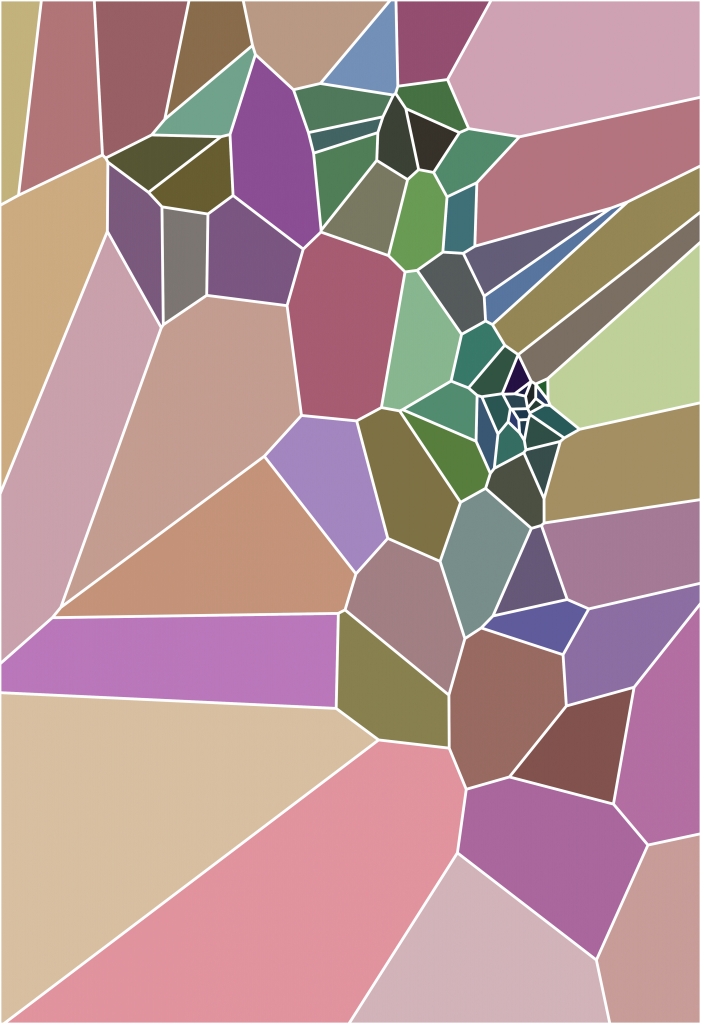
\includegraphics[width=\paperwidth, height=\paperheight]{imagens/ChicagoCrime.png}
  }%
}
\usepackage{booktabs}
\usepackage{longtable}
\usepackage{array}
\usepackage{multirow}
\usepackage{wrapfig}
\usepackage{float}
\usepackage{colortbl}
\usepackage{pdflscape}
\usepackage{tabu}
\usepackage{threeparttable}
\usepackage{threeparttablex}
\usepackage[normalem]{ulem}
\usepackage{makecell}
\usepackage{xcolor}

\begin{document}

\pagenumbering{gobble}

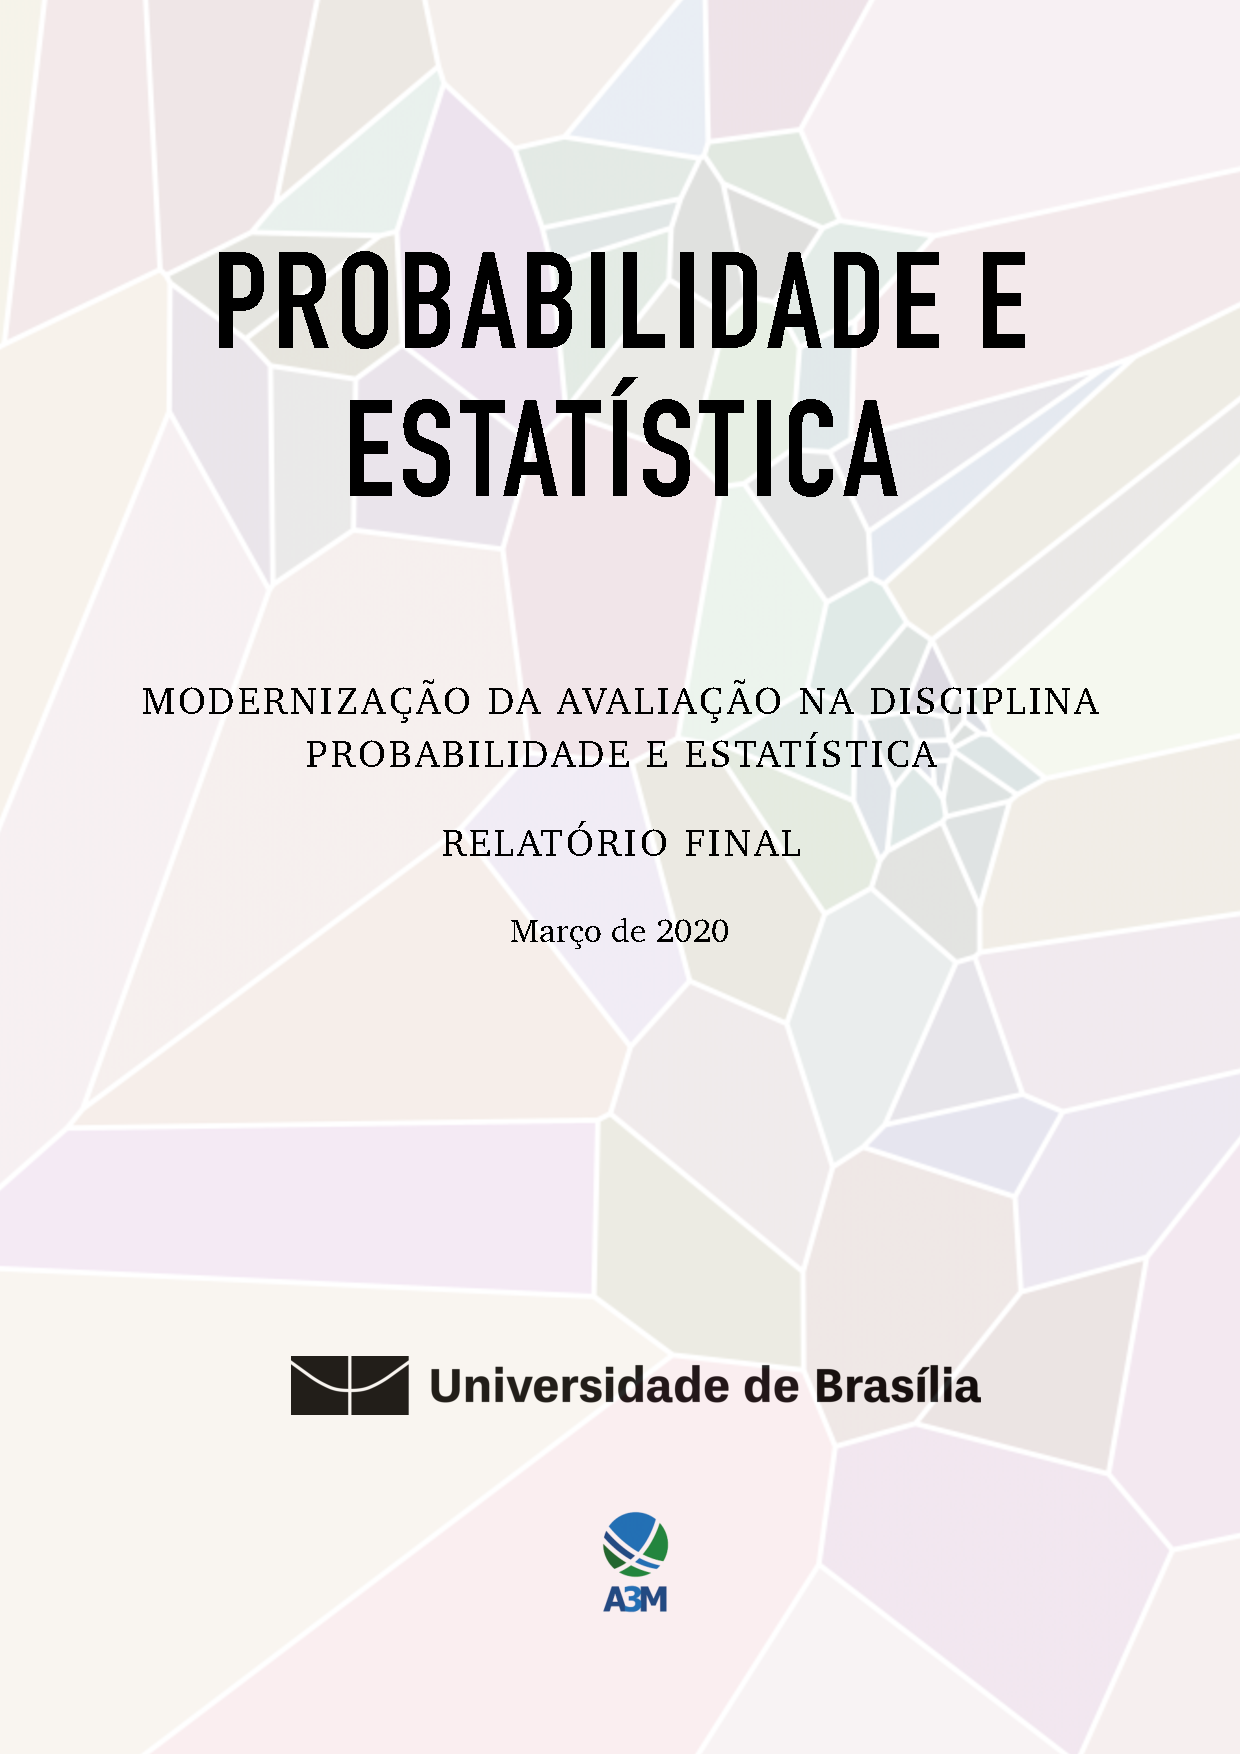
\includepdf[fitpaper=TRUE, pages={1-4}]{CapaRelatorio.pdf}

\pagenumbering{arabic}

\tableofcontents

\newpage

\BgThispage
\chapter{Introdução}

\newpage

O Departamento de Estatística (EST) da UnB oferece semestralmente, em
média, 10 turmas de Probabilidade e Estatística, totalizando
aproximadamente 500 alunos de diversos cursos da área das Ciências
Exatas, incluindo Ciências Econômicas, Química, Matemática, Computação e
diversas Engenharias. A partir do segundo semestre de 2017, com a
unificação da disciplina aprovada na 490ª Reunião Ordinária do Colegiado
do Departamento de Estatística, todos os professores passaram a adotar a
mesma ementa e o mesmo sistema de avaliação, visando a padronização do
curso oferecido e as vantagens decorrentes.

Para tanto, surgiu a necessidade da aplicação de provas unificadas a
todos os alunos matriculados na disciplina. Obviamente, turmas de
dias/horários diferentes não podiam fazer a mesma avaliação. Diante
desse desafio, uma opção operacionalmente onerosa era reunir todos os
alunos simultaneamente para aplicação dos exames. Algumas tentativas
ocorreram aos sábados, mas foram majoritariamente frustradas por
diversas razões logísticas. Tal estratégia demandava a elaboração de
provas que seguiam certa padronização, mas que deveriam ser
suficientemente distintas. Esse processo de elaboração e de correção
manual era demasiadamente dispendioso devido ao número de turmas e de
alunos envolvidos.

No momento da unificação, decidiu-se adotar provas exclusivamente
objetivas, de múltipla escolha. Embora haja mérito na discussão das
vantagens e desvantagens de cada tipo de prova: \emph{aberta},
\emph{fechada} ou \emph{híbrida}, intencionalmente evitamos incluir esse
debate no escopo do projeto.

Simultaneamente a esse movimento do Departamento de Estatística da UnB,
e diante dos mesmos desafios aqui encontrados, um grupo de pesquisadores
da Universidade de Economia e Negócios de Viena, liderados pelo
Professor Achim Zeileis, criaram uma biblioteca de funções em linguagem
\texttt{R}, batizada como \emph{R/Exams}, que permite a automação das
fases de elaboração e correção de provas em cursos de graduação. Entre
outras inúmeras funcionalidades, o pacote permite que os valores
contidos no enunciado de cada questão sejam gerados aleatoriamente, de
modo que cada aluno tenha uma prova específica, diferente das demais.
Além do desejável efeito na redução do risco de fraudes, tal abordagem
garante longevidade ao banco de questões, uma vez que não basta ao aluno
decorar as respostas, mas sim dominar todos os passos necessários para
se chegar à solução desejada.

A cada nova aplicação das provas no formato proposto, um valioso
conjunto de dados se torna disponível, permitindo, entre outros usos, a
calibração prévia do nível de dificuldade das provas, a identificação de
temas de ensino com aproveitamento deficitário, a avaliação longitudinal
do desempenho dos alunos, e, de maneira mais ampla, a consistência na
execução do projeto pedagógico nas diversas turmas.

A necessidade dessa automação se tornou clara para a disciplina de
Probabilidade e Estatística. Provas individualizadas e padronizadas se
mostraram uma solução robusta para o sistema de avaliação. Todo material
produzido está disponível sob consulta para outras Universidades,
podendo ser aplicado diretamente em cursos de Estatística básica ou
adaptado para qualquer outra disciplina com provas de múltipla escolha.

\section{Objetivos}

Este projeto modernizou e otimizou o sistema de avaliação dos alunos do
curso de Probabilidade e Estatística da UnB, incluindo todas as suas
fases: elaboração, impressão, aplicação, correção, divulgação e revisão
das provas.

Os objetivos específicos estão elencados a seguir.

\begin{itemize}
\tightlist
\item
  Redução dos custos operacionais, em especial na construção e na
  correção das provas, por meio do reaproveitamento das questões
  elaboradas e da automação da correção.
\item
  Construção de um extenso e variado banco de questões (com possível
  aproveitamento em outras disciplinas de Estatística básica e/ou em
  cursos semipresenciais ou a distância).
\item
  Estabelecimento de metodologias de análise das respostas dos alunos,
  via Teoria da Resposta ao Item, para o aperfeiçoamento contínuo do
  sistema e da qualidade do banco de questões;
\item
  Criação de rotinas computacionais para viabilizar e automatizar as
  soluções desenvolvidas ao longo do projeto (extensão do pacote
  \emph{R-exams});
\item
  Elaboração de relatórios gerenciais para professores e coordenadores
  da disciplina (vide Capítulo \ref{cap:AnaliseTRI});
\item
  Promoção da consistência na execução do projeto pedagógico nas
  diversas turmas, incluindo a equalização do nível de dificuldade das
  provas nas diversas turmas;
\item
  Aumento da transparência e da agilidade na divulgação dos resultados
  (os alunos têm acesso ao espelho e à solução detalhada de sua prova);
\item
  Simplificação da logística de impressão, aplicação e revisão dos
  exames;
\item
  Redução do risco de fraudes;
\end{itemize}

\section{Desenvolvimento}

O projeto contou com a participação de dois alunos bolsistas
(financiados pelo Programa Aprendizagem para o 3º Milênio (A3M) da UnB)
por um período de 12 meses. Ambos trabalharam na construção de um banco
com 300 questões de Estatística básica no formato requerido pela
ferramenta R/Exams, contendo: enunciado, funções matemáticas que geram
as alternativas, descrição detalhada da solução e especificação dos
procedimentos de geração dos valores aleatórios (que variam de aluno
para aluno). A análise apresentada no Capítulo \ref{cap:AnaliseTRI} foi
elaborada como parte de um Projeto de iniciação científica (PIBIC),
financiado pela FAPDF, e de um Trabalho de Conclusão de Curso (TCC).

O projeto teve também participação de uma equipe de professores (ver
detalhes na capa), os quais contribuíram enormemente na proposição de
modelos de perguntas e num rigoroso processo de revisão das questões.
Além de supervisionar os alunos citados, o Professor Guilherme,
coordenador do projeto, trabalhou na extensão das funcionalidades
computacionais da ferramenta R/Exams, a fim de facilitar a
operacionalização das provas e automatizar as atividades intermediárias
inerentes ao processo.

\section{Aspectos gerais do sistema} \label{sec:sistema}

Buscando um sistema de avaliação automatizado, com provas
individualizadas, a comissão de planejamento unificado da disciplina de
Probabilidade e Estatística optou por adotar como ferramenta primária de
avaliação o pacote computacional livre Exams
(\url{http://www.r-exams.org}).

Entre as principais funcionalidade do pacote R-exams está a
aleatorização dos parâmetros do enunciado das questões conforme
especificação do usuário. Ou seja, números aleatórios são gerados para
compor o enunciado do problema. Dessa forma, ainda que a mesma questão
apareça em provas diferentes, o aluno deverá compreender todos os passos
do raciocínio para chegar ao resultado correto.

Todas as questões do banco foram elaboradas meticulosamente para
permitir essa aleatorização. A especificação do procedimento de
amostragem dos parâmetros é uma atividade delicada e determinante para
garantir que todas as amostras gerem enunciados que sejam válidos e
razoáveis. A definição das funções matemáticas que geram as alternativas
também requer cuidado - caso contrário há o risco de haver alternativas
iguais ou absurdas.

O processo de revisão do banco também foi igualmente importante para
suprimir eventuais falhas de lógica ou de programação. Visando
demonstrar a aplicabilidade do conteúdo teórico nas diversas áreas de
atuação dos futuros profissionais, a contextualização do enunciado das
questões foi fator primordial na construção desse material. O banco
atualmente conta com 300 modelos de questão, todos eles escritos em
linguagem R, versando sobre 30 tópicos de Estatística básica. Este banco
pode ser utilizado em outras disciplinas de Estatística básica e está
disponível sob consulta.

Além do banco de questões, o sistema conta com um arcabouço de funções
em linguagem R, como extensão ao pacote R-exams, para ampliar as suas
funcionalidades e facilitar a interface com o usuário. Os parâmetros que
podem ser modificados para atender necessidades específicas são:

\begin{itemize}
\tightlist
\item
  Número de questões na prova;
\item
  Pontuação de cada questão;
\item
  Escolha dos tópicos (dentre 30 opções atualmente disponíveis);
\item
  Número de turmas e quantidade de alunos em cada turma.
\end{itemize}

Quanto à estrutura de avaliação da disciplina Probabilidade e
Estatística na UnB, esta é composta por 3 provas regulares (com pesos
30\%, 30\% e 40\%) e uma prova substitutiva (abrangendo todo o conteúdo
do curso) para alunos que desejem repor uma eventual prova não realizada
ou queiram substituir a menor nota (entre as provas regulares). Cada
avaliação contém 10 questões de múltipla escolha sobre 10 tópicos
pré-estabelecidos. Sendo assim, para cada turma, o sistema desenvolvido
sorteia 10 questões do banco (uma de cada tópico). Assim, apesar de
turmas diferentes realizarem provas diferentes, a fixação dos tópicos
garante uniformidade no conteúdo cobrado nas avaliações. Em princípio,
também é possível sortear 10 questões diferentes (ainda uma de cada
tópico) para cada aluno do curso, mas considerando a aleatorização do
enunciado, essa opção foi considerada inapropriada por inviabilizar a
revisão em sala das questões feitas pelos alunos da turma.
Alternativamente, poder-se-ia garantir que não há questões que se
repetem em mais de uma turma. Tal estratégia também foi considerada
inoportuna por comprometer o uso da TRI, uma vez que sem questões
repetidas, não seria possível comparar os resultados obtidos nas
diferentes turmas.

Após a aplicação do exame, as folhas de resposta dos discentes são
escaneadas e então corrigidas automaticamente pelo sistema, o qual, ao
identificar o número do documento (prova), executa a correção
considerando o gabarito que lhe é próprio. Ao suspeitar de erro de
marcação ou de leitura do cartão de respostas, a plataforma solicita ao
operador a conferência manual dos dados.

Como subproduto do processo de correção das provas, o sistema produz
resultados de forma individualizada. Mais especificamente, cada aluno
recebe um documento (em formato \emph{pdf}) contendo uma cópia da sua
folha de respostas, o gabarito resumido e a solução detalhada da sua
prova específica. Para acessar o arquivo, disponibilizado no Moodle, o
aluno usa como senha o número da prova, impresso em seu caderno de
questões (que o aluno leva consigo ao final da prova). Considerando a
dimensão atual do banco de dados e a aleatorização dos enunciados, não
há prejuízo que os alunos tenham acesso a provas antigas.

A avaliação do desempenho dos alunos nesse nível de riqueza e
profundidade é inédita no âmbito do Departamento de Estatística da UnB,
e possivelmente em toda a Universidade de Brasília.

Maiores detalhes a respeito da utilização do sistema (passo-a-passo)
encontram-se no Capítulo \ref{cap:Manual}.

\section{Descrição dos produtos entregues}

Os produtos produzidos nesse projeto estão sumarizados a seguir:

\textbf{1. Banco de questões}

O banco possui 300 modelos de questões de Estatística básica,
organizadas em 30 temas. Cada questão contém a descrição do procedimento
amostral para geração dos parâmetros aleatórios envolvidos, o enunciado,
as funções que geram as alternativas erradas e a solução detalhada da
questão.

\textbf{2. Relatório de análise dos dados (Capítulo
\ref{cap:AnaliseTRI})}

Relatório com análise dos dados produzidos com a aplicação do sistema na
disciplina de Probabilidade e Estatística (a partir da leitura dos
cartões de respostas).

\textbf{3. Manual de utilização do sistema (Capítulo \ref{cap:Manual})}

O manual descreve detalhadamente o procedimento de geração e correção
das provas utilizando o código disponível em linguagem \texttt{R}.

\textbf{4. Códigos do sistema}

Os códigos desenvolvidos estão disponíveis sob consulta.

\newpage

\BgThispage
\chapter[Análise de resultados]{Análise de resultados \\ 2º/2019} \label{cap:AnaliseTRI}

\newpage

A mensuração do aprendizado dos estudantes a partir da realização de
testes é um aspecto fundamental do sistema educacional. O resultado dos
testes fornece a professores, educadores e alunos informações de grande
importância sobre o aprendizado dos discentes. Tal medida é utilizada,
por exemplo, para determinar se o aluno deve ou não ser aprovado no
curso.

Tradicionalmente, pela simplicidade de sua formulação, a Teoria Clássica
dos Testes (TCT) é adotada para este fim. Em resumo, nessa abordagem,
entende-se que a pontuação do aluno (escore observado) corresponde à
soma da pontuação esperada (resultado da \emph{habilidade latente} do
aluno) e do erro amostral (que faz com que o desempenho varie caso o
aluno seja hipoteticamente submetido a diversas provas sobre o mesmo
conteúdo e com o mesmo nível de dificuldade). Ou seja, a nota obtida é
um estimador natural da \emph{proficiência} do aluno.

A habilidade latente (um atributo mental não observável do respondente),
por sua vez, resulta de diversos fatores, dentre os quais destacamos o
potencial cognitivo do aluno, sua dedicação ao curso, seus métodos de
estudo e a experiência em sala de aula (composição da turma, estrutura
física, horário, didática adotada pelo professor, materiais didáticos
utilizados, entre outros fatores).

Recentemente, a Teoria de Resposta ao Item (TRI) vem ganhando espaço, em
detrimento da Teoria Clássica dos Testes, sobretudo para testes de
grande escala. De acordo com o Ministério da Educação, ``No Brasil, a
TRI é usada desde 1995 nas provas do Sistema Nacional de Avaliação da
Educação Básica (Saeb), que mede o desempenho de estudantes do ensino
fundamental e médio. Em 2009, foi usada pelo Enem com o objetivo de
garantir a comparação das notas do exame daquele ano com os seguintes.''
No exterior, exames como o \emph{Test of English as a foreign language}
(TOEFL) adotam a TRI há mais de 50 anos. A TRI é aplicável a diversos
campos das Ciências e, para além do campo educacional, se mostrou
particularmente útil na Medicina e na Psicometria.

Os modelos de TRI buscam estimar, a partir do ajuste de modelos
estatísticos, a probabilidade de um aluno responder corretamente a um
item em função de suas características (habilidades) e dos atributos do
próprio item. A abordagem probabilística permite que se leve em
consideração, entre outros aspectos, o nível de dificuldade e o poder de
discriminação do item (uma medida do quanto a probabilidade de acerto
varia em função do aumento da habilidade do aluno).

Destacamos que não há intenção de, em um futuro próximo, atribuir menção
em função da habilidade estimada via TRI. Os modelos são empregados
exclusivamente para a investigação de como o processo avaliativo, e em
especial o banco de questões, pode ser aprimorado.

Na Seção \ref{sec:descritiva} apresentamos alguns gráficos que ilustram
o desempenho dos alunos ao longo do semestre e o efeito da prova
substitutiva nas menções. Depois, na Seção \ref{sec:TRI}, introduzimos o
modelo de TRI adotado e apresentamos os principais resultados obtidos.
Por fim, na Seção \ref{sec:conclusao}, listamos as principais conclusões
e recomendações.

\section{Análise descritiva dos dados} \label{sec:descritiva}

\subsection{Desempenho dos alunos}

A Tabela 2.1 apresenta um conjunto de estatísticas do curso. Neste
estudo, apenas são contabilizados os alunos que concluíram o curso, com
ou sem sucesso. As menções apresentadas não correspondem necessariamente
à menção efetivamente atribuída pelo professor, o qual tem a
prerrogativa de considerar outros critérios, como a entrega de listas de
exercícios, a participação do aluno em sala, etc.

A média final (5.8) foi ligeiramente superior à nota média prevista
(5.5), especificada na construção dos testes pela função que amostra as
questões de cada turma, conforme descrito na Subseção
\ref{subsec:sorteio}. Isso se deve ao descarte das respostas dos alunos
que não concluíram o curso. A nota média das diferentes turmas
apresentou pequena variação, diferentemente do que era observado antes
da unificação da disciplina, quando as notas médias das turmas variavam
amplamente. Maior homogeneidade do resultado entre turmas também foi
observada no percentual de aprovados. Entretanto, apenas 4\(\%\) dos
alunos atingiram a menção máxima (SS). Cientes da dificuldade de se
obter nota final igual ou superior a 9 com esse sistema de avaliação,
mesmo após a prova substitutiva, os professores podem considerar outros
aspectos do desempenho dos alunos com nota final próxima de 9.

\begin{longtable}{c|c|c|c|c}
\caption{\label{tab:unnamed-chunk-4}Estatísticas do curso}\\
\hline
Turma & Alunos & Nota final média & \% de aprovados & \% de SS\\
\hline
\endfirsthead
\caption[]{Estatísticas do curso \textit{(continued)}}\\
\hline
Turma & Alunos & Nota final média & \% de aprovados & \% de SS\\
\hline
\endhead
AA & 47 & 5.8 & 76.1 & 8.1\\
\hline
AB & 49 & 5.5 & 65.2 & 8.2\\
\hline
BA & 38 & 5.7 & 72.9 & 2.4\\
\hline
BB & 46 & 6.0 & 77.3 & 6.2\\
\hline
CA & 52 & 6.2 & 83.9 & 10.7\\
\hline
CB & 44 & 5.8 & 74.6 & 0.0\\
\hline
CC & 49 & 5.0 & 63.1 & 0.0\\
\hline
DA & 16 & 5.4 & 74.1 & 0.0\\
\hline
DB & 39 & 5.4 & 64.1 & 0.0\\
\hline
EA & 49 & 5.2 & 64.0 & 0.0\\
\hline
Total & 429 & 5.8 & 71.5 & 4.0\\
\hline
\end{longtable}

A Figura 2.1 apresenta a nota final de cada aluno da disciplina,
discriminada pelo curso do discente. Nota-se que, embora haja certa
similaridade entre os cursos, o desempenho dos alunos de Engenharia
Elétrica, por exemplo, é substancialmente superior ao de cursos
classificados como ``Outros''.

\begin{figure} 
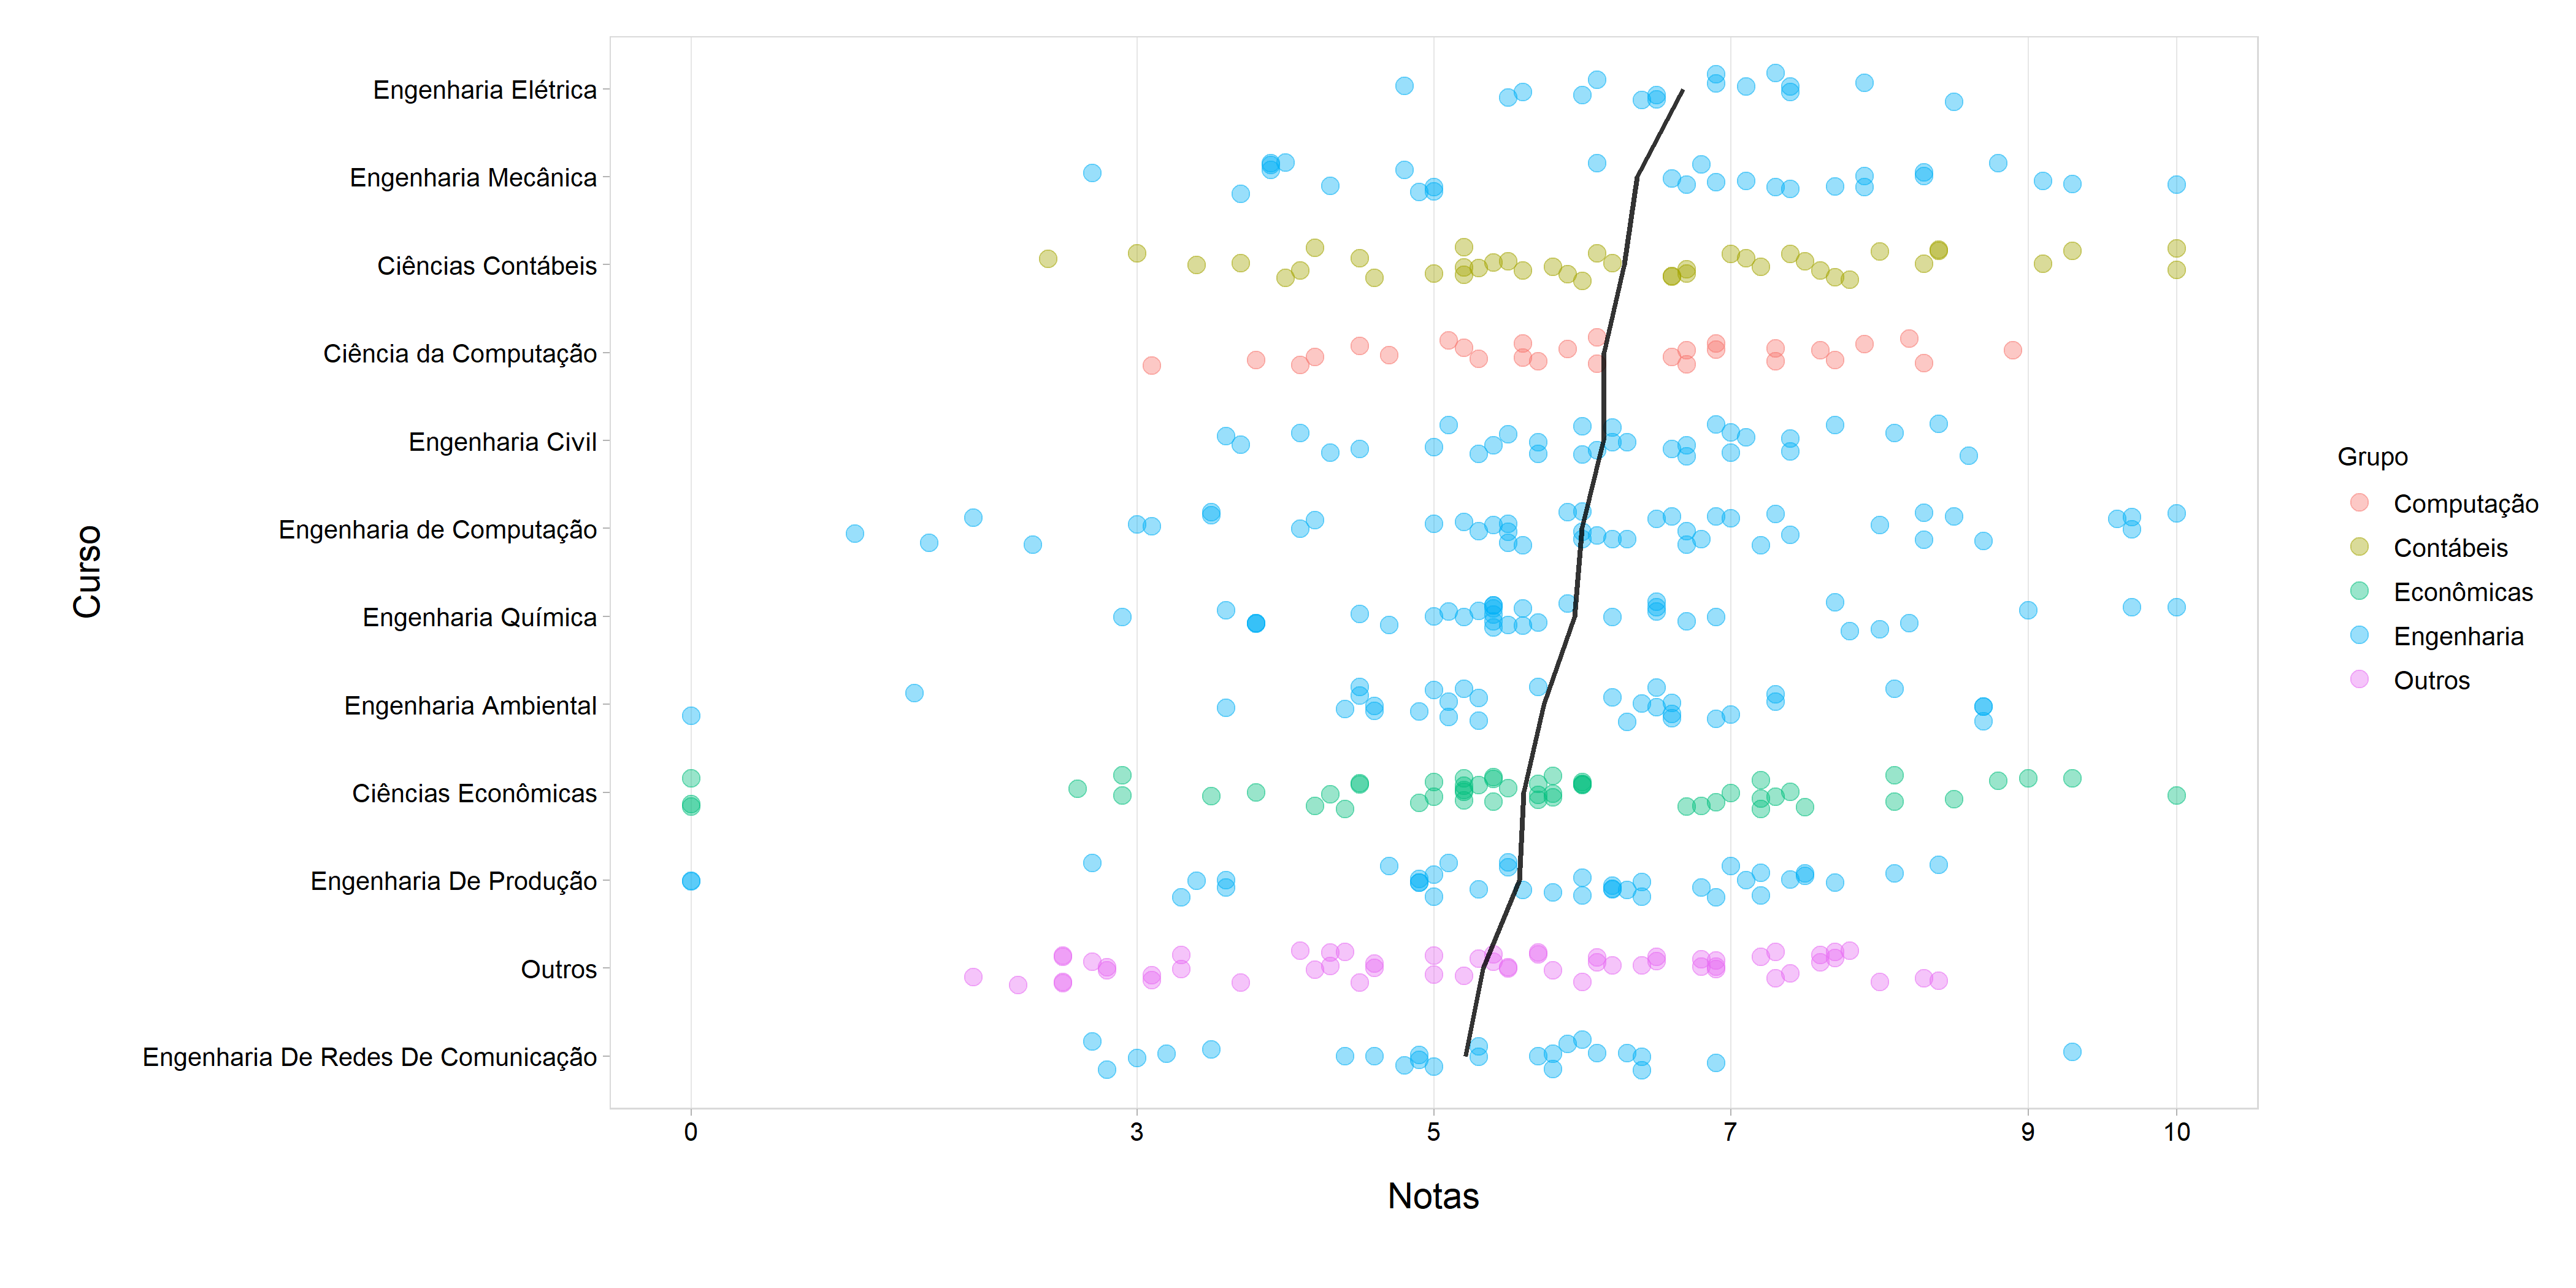
\includegraphics{Notas_cursos.png} 
\caption{Notas finais por curso. Para evitar pontos sobrepostos (quando alunos de um mesmo curso apresentam a mesma nota final), os pontos foram ligeiramente descolados verticalmente (procedimento conhecido como ``jitter"). A linha preta indica a média geral de cada curso.}
\label{fig:notas_cursos}
\end{figure}

A Figura 2.2(a) indica que a Prova 2 é o exame mais difícil ao longo do
semestre. Embora as notas da prova substitutiva também sejam mais
baixas, cabe ressaltar que isso se deve sobretudo ao fato de que os
alunos que se submetem à prova substitutiva, em geral, tiveram
desempenho insatisfatório nas provas anteriores. Os painéis (b), (c) e
(d) mostram o percentual de acerto de cada tópico das Provas 1, 2 e 3,
respectivamente. Ao avaliá-lo com cuidado, os professores podem observar
temas cujo desempenho foi superior ou inferior à média. Em que pese o
resultado da prova depender em grande medida da composição da turma,
temas que se apresentem atipicamente abaixo da média sugerem ao
professor avaliar a necessidade de interferir na estratégia de ensino,
dedicando mais tempo ao tópico, por exemplo.

O tema sobre teste de hipóteses para a proporção teve percentual de
acerto inferior a \(50\%\) em todas as turmas, o que não parece
razoável. Sugerimos, portanto, que se investigue as causas deste
resultado para que se tome as medidas cabíveis. Caso as questões estejam
inapropriadas (voltaremos a esse tema adiante), é preciso melhorar os
modelos de questão. Caso contrário, será preciso buscar maneiras de
aperfeiçoar o ensino nessa frente. Neste contexto, cabe ressaltar que
este é normalmente o último tópico ministrado no curso.

\begin{figure}[!h]
    \centering
  \subfloat[\footnotesize{Nota média por turmas e por prova.}]{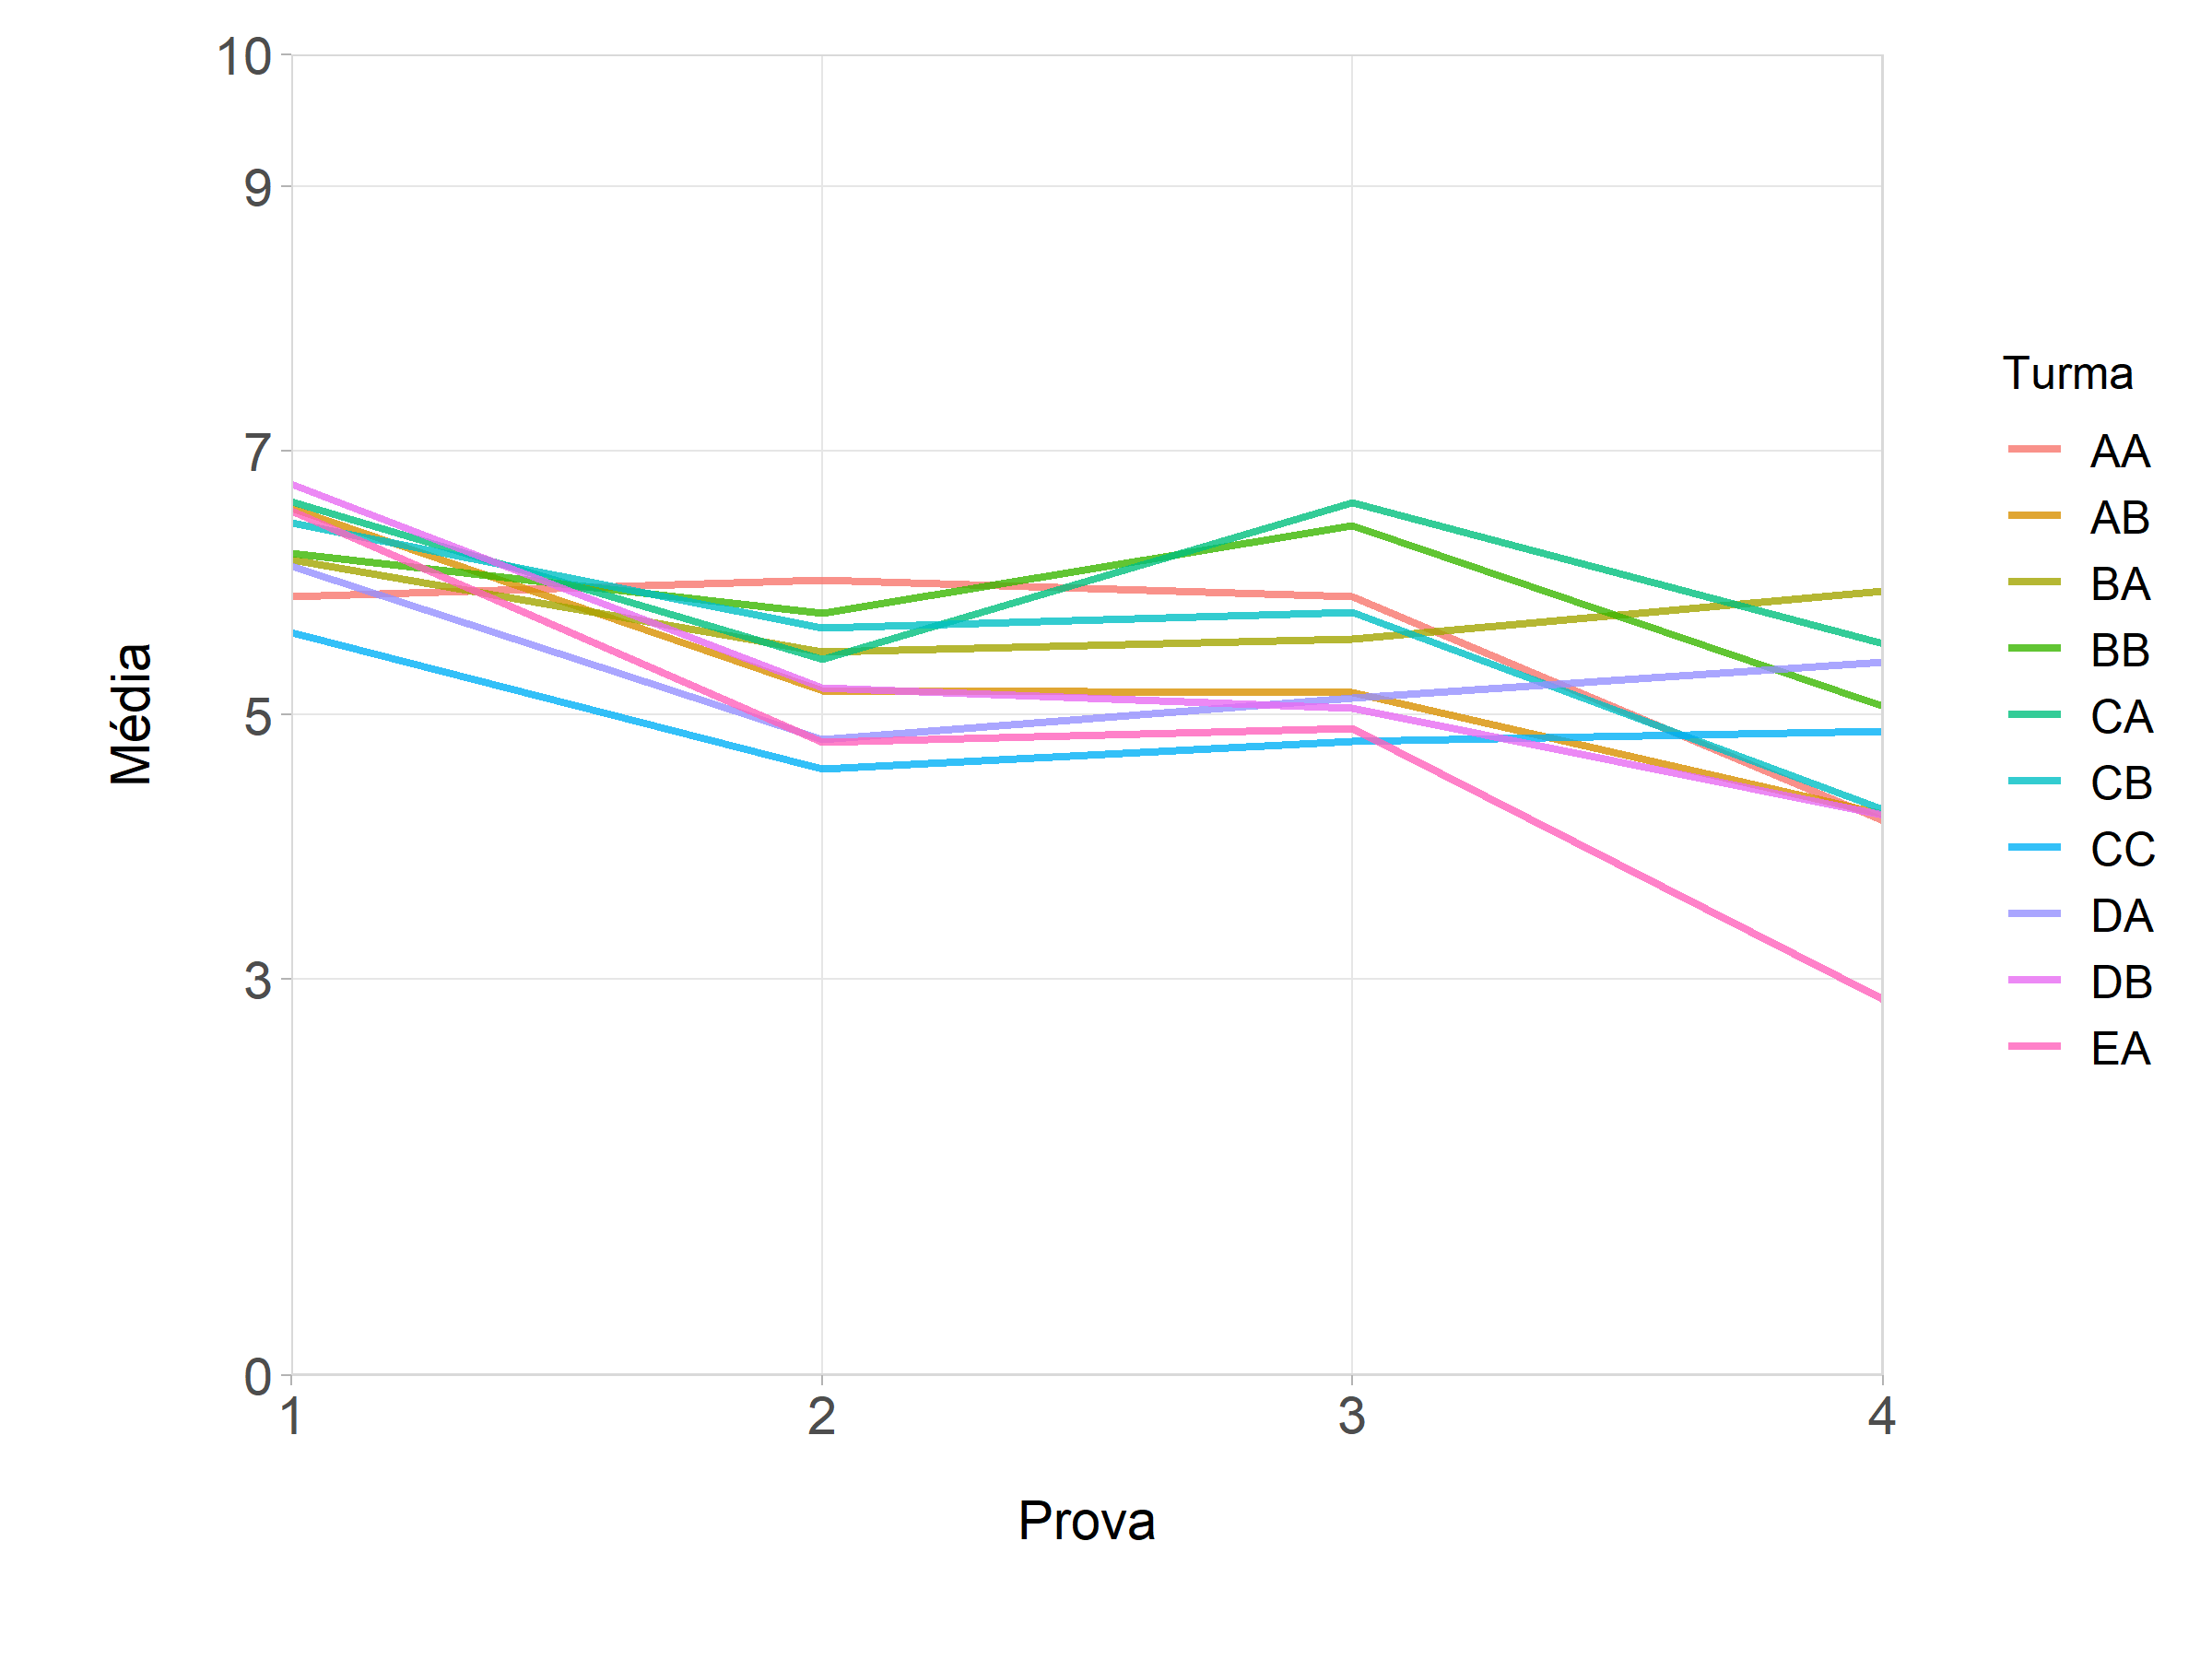
\includegraphics[width=8cm,height=6cm]{Media_provas.png}}
    \subfloat[\footnotesize{Proporção de acertos - Prova 1.}]{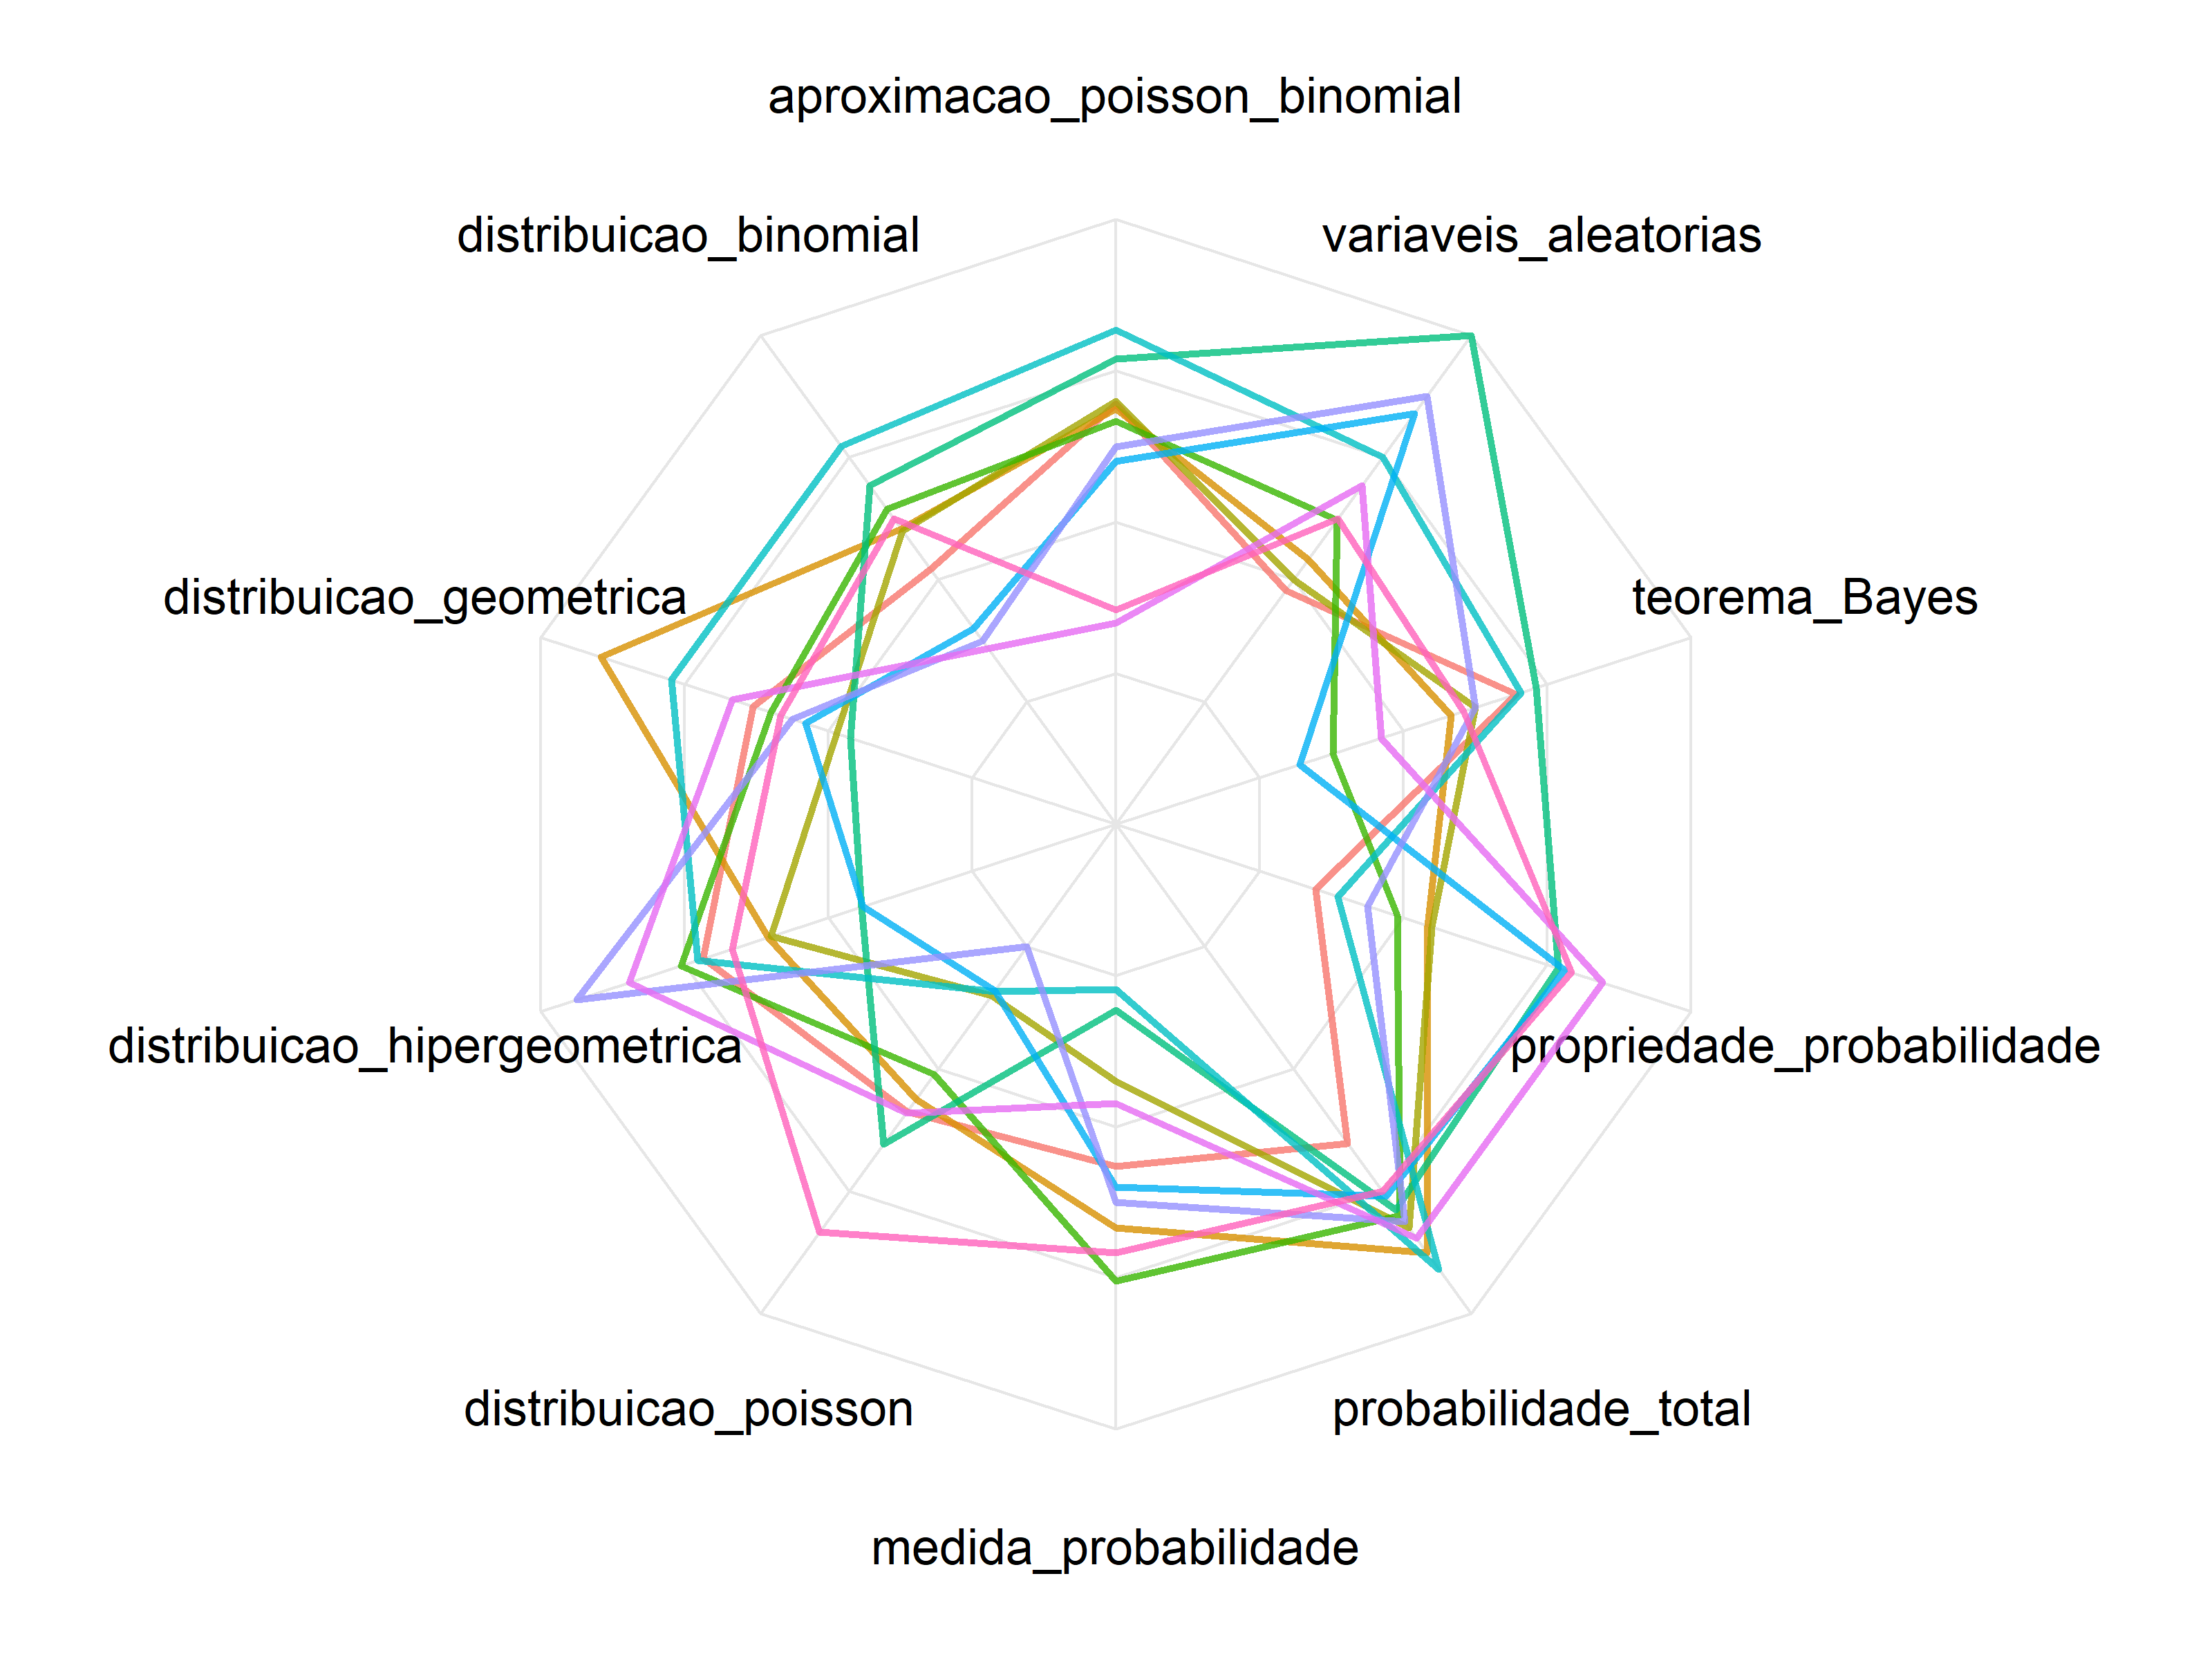
\includegraphics[width=8cm,height=6cm]{g_radar_1.png}} 
    \\
    \subfloat[\footnotesize{Proporção de acertos - Prova 2.}]{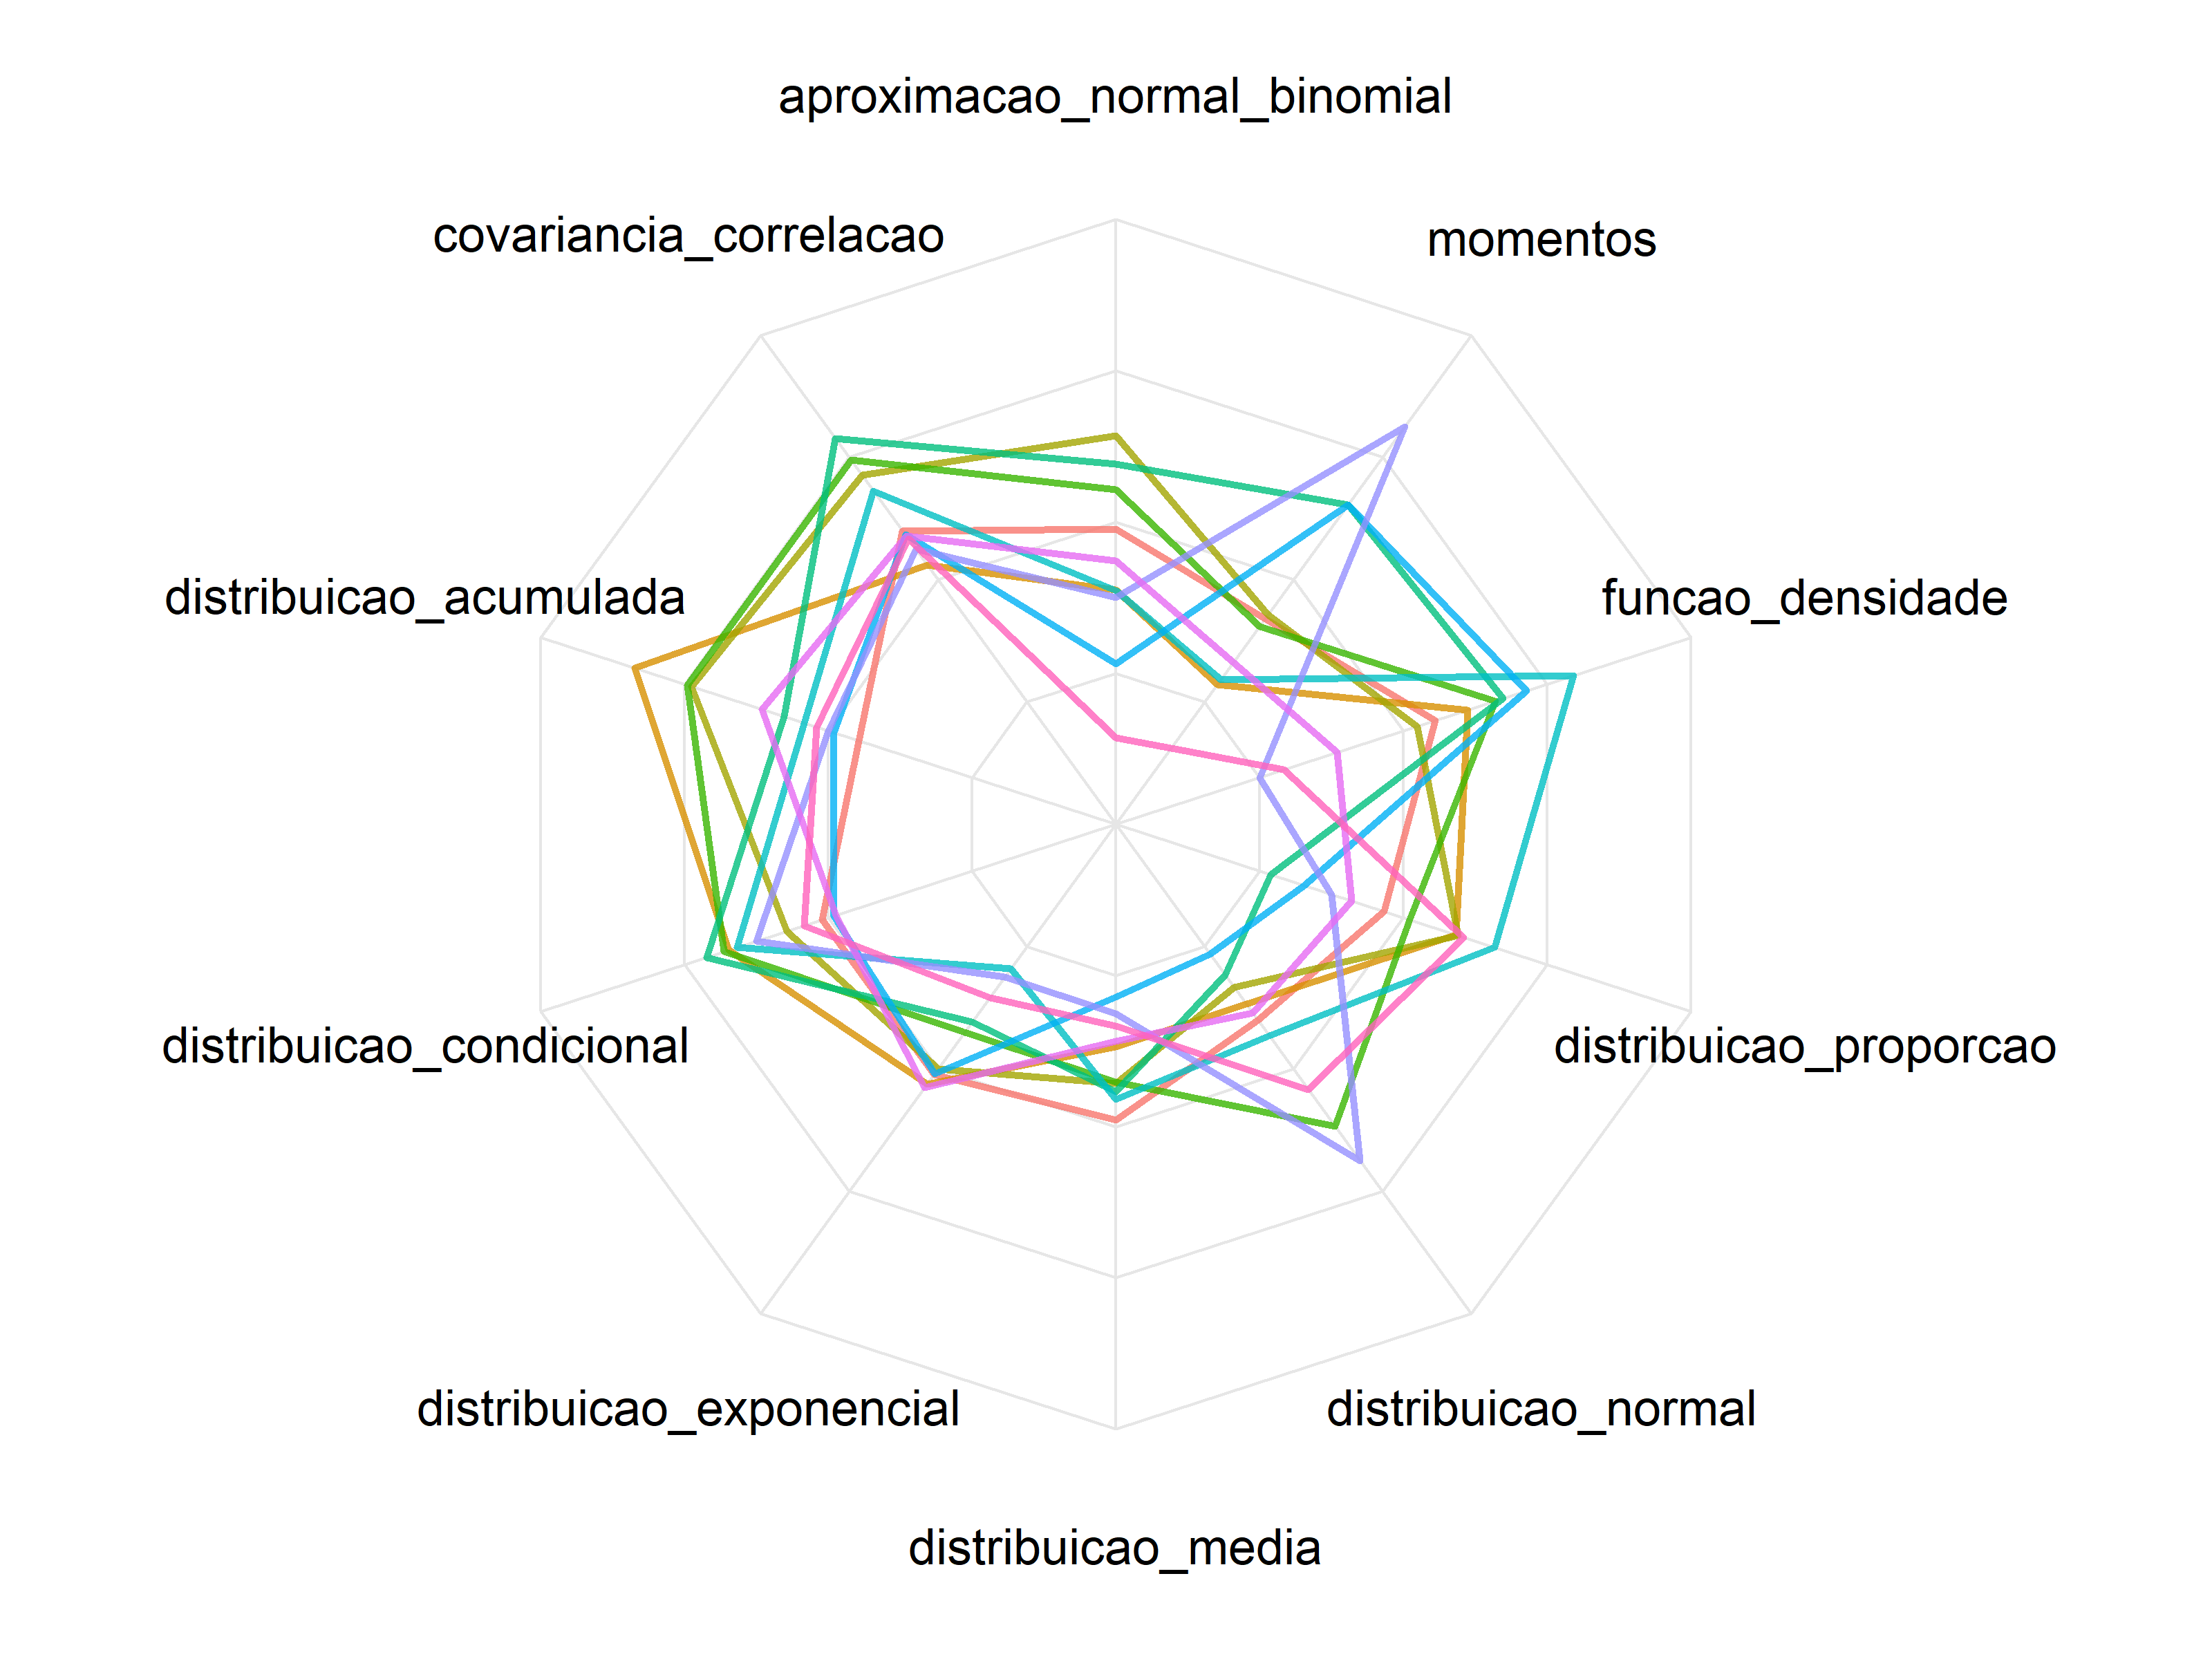
\includegraphics[width=8cm,height=6cm]{g_radar_2.png}}
    \subfloat[\footnotesize{Proporção de acertos - Prova 3.}]{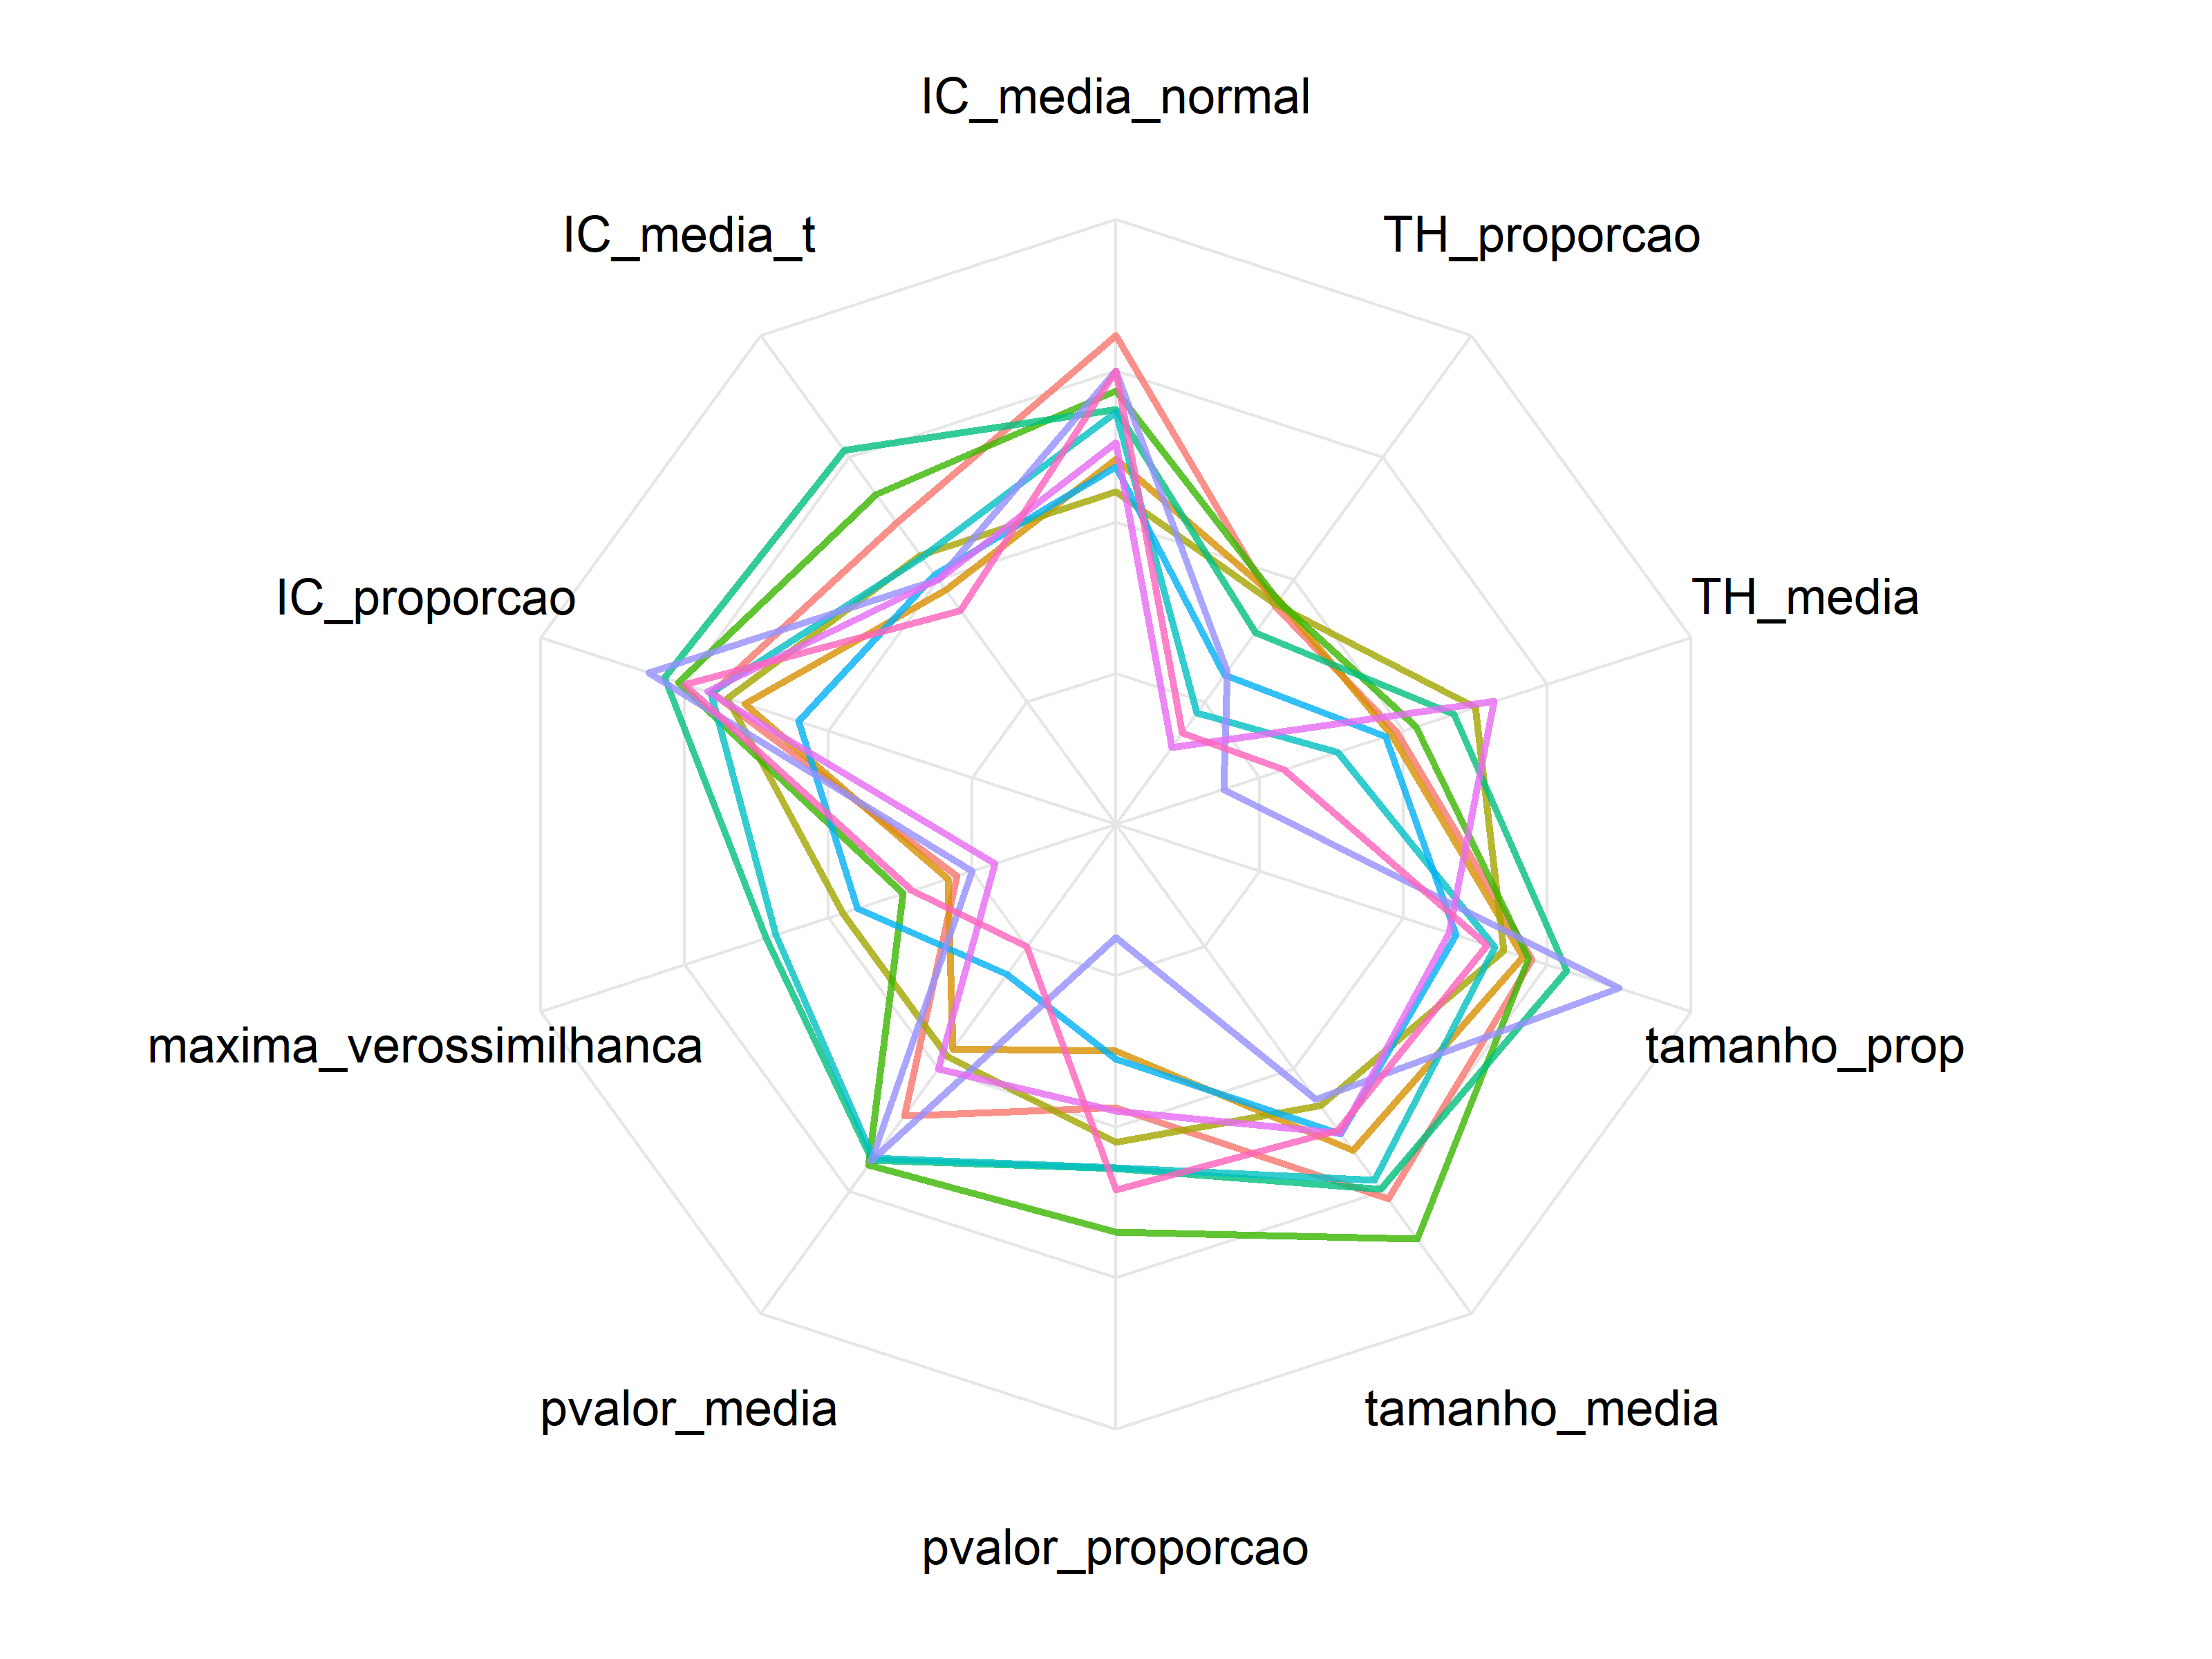
\includegraphics[width=8cm,height=6cm]{g_radar_3.png}}
    \caption{\small (a) Nota final média dos alunos por turma e número da prova. (b), (c) e (d) apresentam, respectivamente, o percentual de acerto por tema nas provas 1, 2 e 3. O centro da figura representa $0\%$ de acerto, enquanto a borda mais externa indica $100\%$. Questões anuladas estão representadas pela média de acerto no respectivo tema.
}
    \label{fig:notas.medias}
\end{figure}

\subsection{Prova substitutiva}

Conforme discutido na Seção \ref{sec:sistema}, os alunos são autorizados
a realizar uma prova substitutiva no final do semestre, versando sobre
todo o conteúdo do curso. A nota da prova substitutiva substitui a menor
nota, desde que a nota final não diminua (por isso ela é conhecida como
``sub do bem'').

A Figura 2.3 traz um resumo visual dos efeitos da prova substitutiva.
Primeiramente, no painel (a), apresentamos o fluxo acumulado parcial das
menções ao longo do curso. Observa-se que a mobilidade entre as menções
é limitada. A menção máxima, por exemplo, é atingida quase
exclusivamente por aqueles que tiveram alto desempenho desde a primeira
prova. A figura (b) retrata o número de alunos com nota final nas
respectivas faixas, com a cor atribuída de acordo com a participação do
aluno na prova substitutiva. Ao todo, 138 fizeram a prova substitutiva,
dos quais 78.3\(\%\) estavam reprovados. Destes, 41.7\(\%\) conseguiram
a aprovação.

\begin{figure} 
    \centering
  \subfloat[\footnotesize{Fluxo das menções.}]{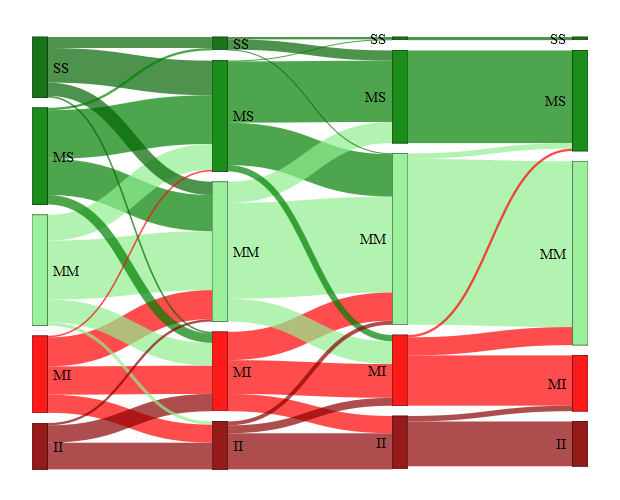
\includegraphics[width=14cm,height=5cm]{sankey.png}}
  \\
    \subfloat[\footnotesize{Número de alunos por faixa (após a Prova 3).}]{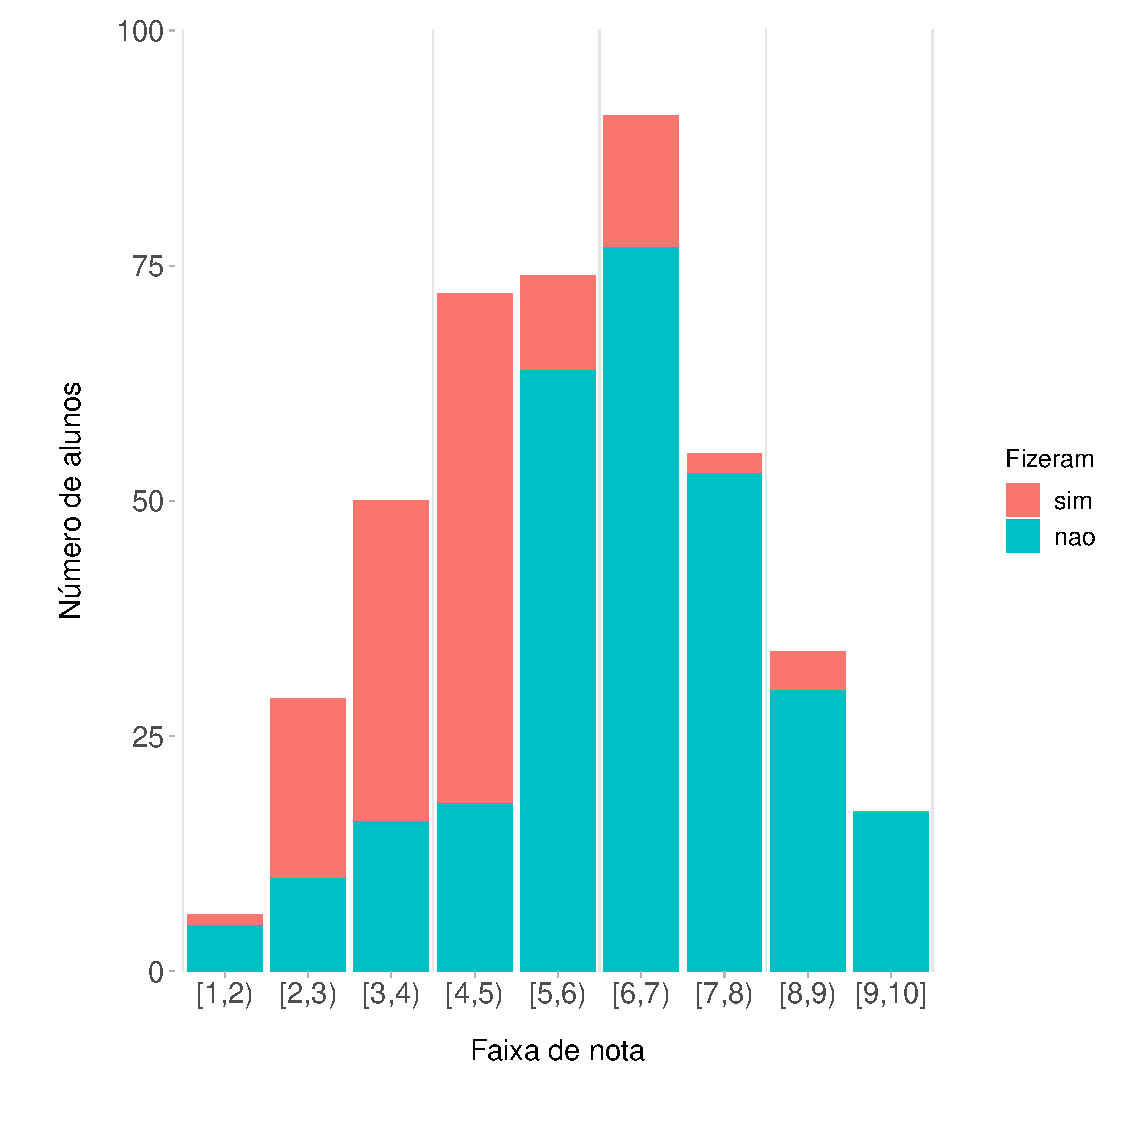
\includegraphics[width=7.5cm,height=7.5cm]{porp_p4.pdf}}
    \subfloat[\footnotesize{Menção antes e depois da Prova substitutíva.}]{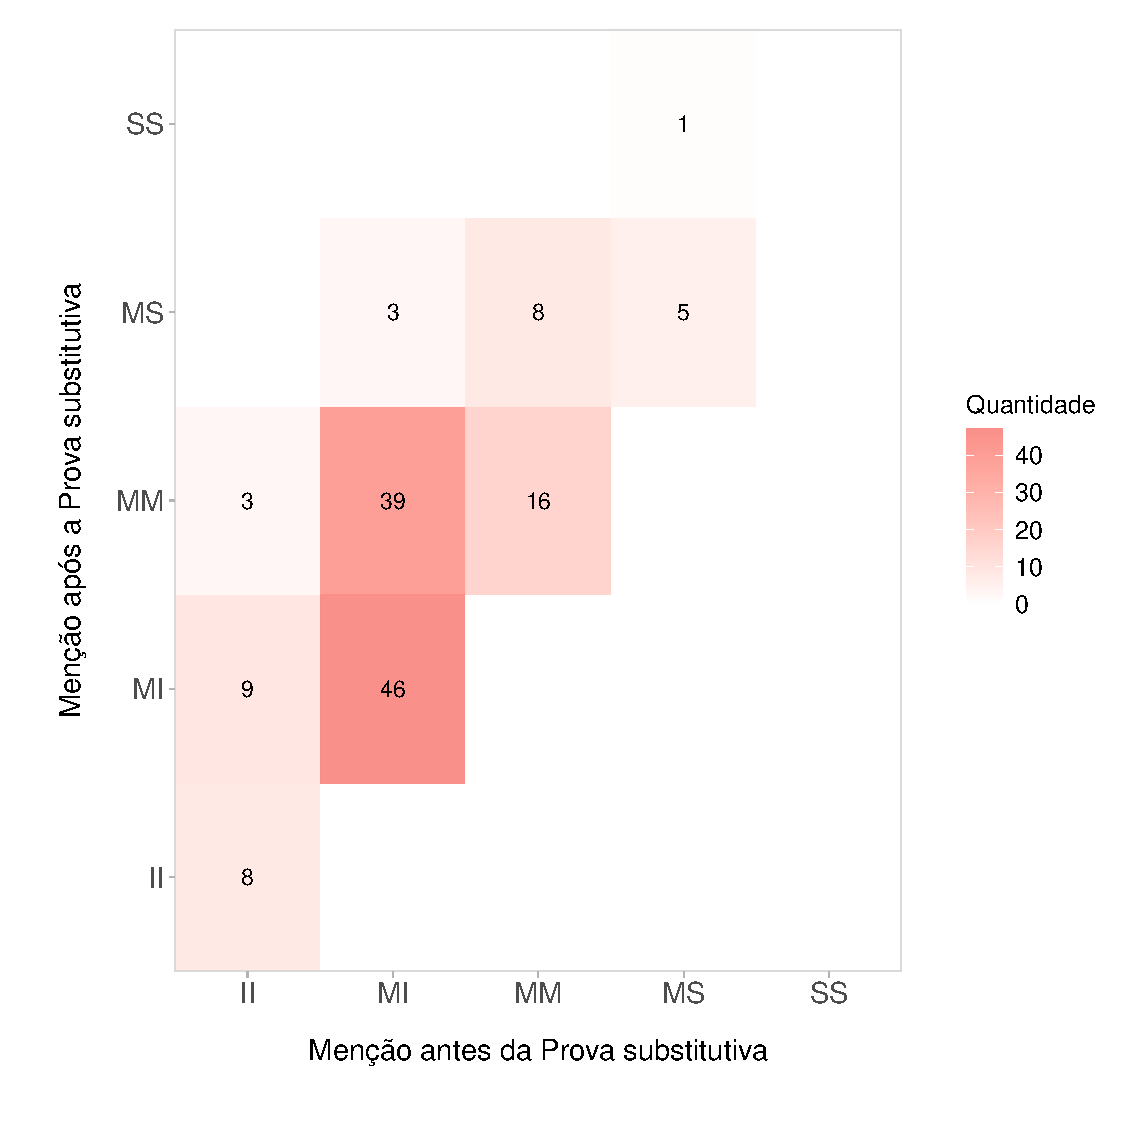
\includegraphics[width=7.5cm,height=7.5cm]{confusao_subs.pdf}}
\caption{(a) Fluxo das menções parciais acumuladas. As quatro barras verticais indicam, na ordem, as 4 provas realizadas no curso. 
Na Prova 1, temos a menção correspondente à nota da própria prova; na Prova 2, calculou-se a menção parcial acumulada a partir da média aritmética das duas primeiras notas; na Prova 3, a nota final foi definida de acordo com os pesos atribuídos na ementa; na Prova substitutiva, tem-se a menção final obtida pelo aluno. Considerou-se apenas alunos que realizaram as 3 primeiras provas. (b) Número de alunos por faixa de nota final após a Prova 3. (c) Matriz com o número de alunos por menção, dada a situação antes e depois da Prova substitutiva.}
\label{fig:notas_cursos}
\end{figure}

\section{Análise via Teoria da Resposta ao Item} \label{sec:TRI}

A simples visualização dos dados brutos já é de grande valia.
Entretanto, para responder questões mais desafiadoras, lançamos mão de
técnicas de modelagem estatística de dados. Entre outras vantagens, o
ajuste de modelos de TRI nos permite traçar um diagnóstico mais completo
do banco de questões. Enquanto o percentual de acerto nos dá indícios
quanto ao nível de dificuldade da questão, ele pouco nos informa sobre a
qualidade das alternativas erradas (se são facilmente descartadas por
alunos de baixa habilidade) e sobre o poder discriminante do item. Além
de evitar questões demasiadamente fáceis ou difíceis, queremos que a
habilidade latente do aluno esteja fortemente associada à probabilidade
de acerto da questão. Caso contrário podemos concluir que o item é pouco
informativo para a habilidade do aluno, o que é o torna sem valor
prático. O percentual bruto de acerto também não leva em consideração
quais alunos responderam ao item. Se ele foi sorteado para uma turma
excelente, por exemplo, um alto valor levaria à falsa impressão de que
se trata de uma questão fácil.

Nesse primeiro momento, ajustamos quatro modelos (um para cada prova),
todos com a mesma estrutura, definida a seguir.

\begin{align*}
Y_{ij} & \sim \text{Ber}(p_{ij}) \\
p_{ij} & = c_j + \frac{1-c_j}{1+\exp(- (a_j\theta_i - b_j))} \\
a_j & \sim \text{Half-normal}(0, 1) \\
b_j & \sim \text{N}(0, 1) \\
c_j & \sim \text{Beta}(5, 17) \\
\theta_i & \sim \text{N}(0, 1),
\end{align*}

onde \(Y_{ij}\) representa se o aluno \(i\) acertou (1) ou errou (0) a
questão \(j\), \(p_{ij}\) a probabilidade do aluno \(i\) acertar a
questão \(j\), \(c_j\) a probabilidade de acerto de um aluno sem
proficiência, \(a_j\) o poder discriminante da questão \(j\), \(b_j\) a
dificuldade do item \(j\) e \(\theta_i\) a habilidade latente do aluno
\(i\).

Note que, com este conjunto de modelos, precisamos estimar
\(3*228 + 3*435 = 1989\) parâmetros valendo-se das 13779 respostas
(pares alunos/questões), o que não é tarefa fácil. Para tanto, usamos o
pacote \emph{RStan}, do \texttt{R}, para gerar amostras da distribuição
a posteriori.

Assumimos que a aleatorização dos números nos enunciados não altera os
atributos (parâmetros) das questões. Além disso, para qualquer par de
questões, dada a habilidade do aluno e os parâmetros das questões, os
resultados (acertou/errou) são independentes um do outro.

\subsection{Resultados preliminares}

Um dos desafios na construção dos testes é garantir certo equilíbrio
entre as turmas. Caso as provas sejam mal calibradas, a nota esperada de
um dado aluno pode ser muito diferente dependendo da turma em que ele
esteja matriculado. Não é razoável, por exemplo, que a nota dependa mais
das questões que foram sorteadas para sua turma do que de sua
proficiência.

A Figura 2.4(a) apresenta a nota média estimada de um aluno mediano (com
habilidade maior que exatamente 50\% dos alunos) nas diversas turmas.
Notadamente, quando se observa uma prova específica, a variação entre as
turmas é apreciável. Entretanto, quando se avalia a dificuldade média
nas 4 provas, conclui-se que a variação entre as turmas é bastante
discreta.

Na Figura 2.4(c), apresentamos a \emph{informação} dos testes, uma
medida que indica o quanto as respostas ``desvendam" a habilidade
não-observável do aluno. Além disso, tal medida esclarece em qual
intervalo de habilidade as respostas são mais informativas. Se, por um
lado, as turmas parecem estar bem balanceadas no que diz respeito ao
nível de dificuldade das questões, por outro, percebe-se que algumas
provas são menos informativas que outras. Nesses casos, mesmo que o
aluno tenha respondido 40 itens ao longo do curso, a incerteza a
respeito de sua proficiência será alta, prejudicando o processo
avaliativo. Nesse sentido, sugerimos que, no momento do sorteio das
questões, se verifique também se as provas estão igualmente
informativas.

A Figura 2.4(b) compara a avaliação adotada pela ementa com o que
obtemos, mantidas as quantidades de alunos em cada menção, ao ordenar os
alunos pela média ponderada das habilidades estimadas. Enquanto a maior
parte dos discentes não teria sua menção alterada, há diversos alunos
que passariam da condição de reprovado para aprovado.

A diferença se deve, sobretudo, a dois fatores. Primeiro,
independentemente do método, há um intervalo de incerteza em torno da
estimativa pontual. Por exemplo, quando o modelo estima uma habilidade
igual a um, ele também entende que a habilidade poderia ser de 0.9 ou
1.1, digamos. Daí, alunos que estejam no limite das menções acabam
eventualmente mudando de faixa dependendo do método adotado. A incerteza
pode ser reduzida aumentando-se o número de questões, mas isso tende a
aumentar os custos operacionais. De todo modo, isso vale para lembrar
que o acaso é um componente não-negligenciável da nota do aluno, e que
outros critérios além da nota podem ser adotados.

Segundo, na TRI leva-se em conta exatamente quais questões foram
acertadas, e não apenas o número total de acertos. Por isso, o escore
estimado tendo a ser maior quando o aluno acerta mais questões difíceis
ou com maior poder de discriminação. Considere o seguinte exemplo.
Suponha que uma das questões da prova de Estatística seja sobre técnicas
de fotografia. Nesse caso, a habilidade do aluno em Estatística não
alteraria a probabilidade do acerto deste item. Por isso, o modelo de
TRI concluiria que o item é pouco informativo para a habilidade
(\(a_j \approx 0\)). Daí, o acerto ou erro do item pouco alteraria a
habilidade estimada pelo modelo. Entretanto, na forma corrente de
avaliação, o acerto do item aumentaria em 1 a nota do aluno, da mesma
forma que ocorreria com qualquer uma das outras questões da prova.

A Figura 2.5(a) apresenta o correlograma dos \emph{resíduos} do modelo
(medida de discrepância entre o valor previsto pelo modelo, \(p_{ij}\) e
o valor observado \(Y_{ij}\)) por tema. Visto que o modelo assume
implicitamente que \(Y_{ij}|p_{ij}\) e \(Y_{lm}|p_{lm}\), são
independentes, para qualquer \(i \neq l\) e \(j \neq m\), é esperado
(pelo modelo) que as correlações sejam próximas a zero. Entretanto, como
a referida suposição não é plenamente válida, observa-se algumas regiões
de coloração mais intensa. Note que a correlação se dá entre os
resíduos, e não sobre os temas diretamente. Por isso, não se pode
concluir, por exemplo, que os temas \emph{Distribuição normal} e
\emph{Intervalo de confiança para a média} são independentes entre si,
mas sim que a informação de quanto o modelo ``errou'' no primeiro tema
não está probabilisticamente associado ao quanto o modelo irá errar no
segundo tema.

Baseado no correlograma, construímos uma rede de associação entre os
resíduos. O resultado está disponível na Figura 2.5(b). Os temas da
Prova 1 estão separados por uma linha imaginária dos temas da Prova 3,
indicando que, para essas provas, os temas estão mais relacionados entre
si. Cabe esclarecer, entretanto, que a distância entre os pontos não
corresponde exatamente ao valor da correlação do par.

As questões do tema \emph{Estimação de máxima verossimilhança}
sabidamente envolvem procedimentos e entendimentos de certo modo
descolados dos demais temas da Prova. No entanto, o mesmo não pode ser
dito sobre o tema de \emph{Teste de hipóteses para a proporção}. Por
isso, novamente sugerimos que se investigue as os motivos que tornaram o
comportamento desse tema contraintuitivo.

\begin{figure} 
    \centering
    \subfloat[\footnotesize{Nota esperada de um aluno mediano.}]{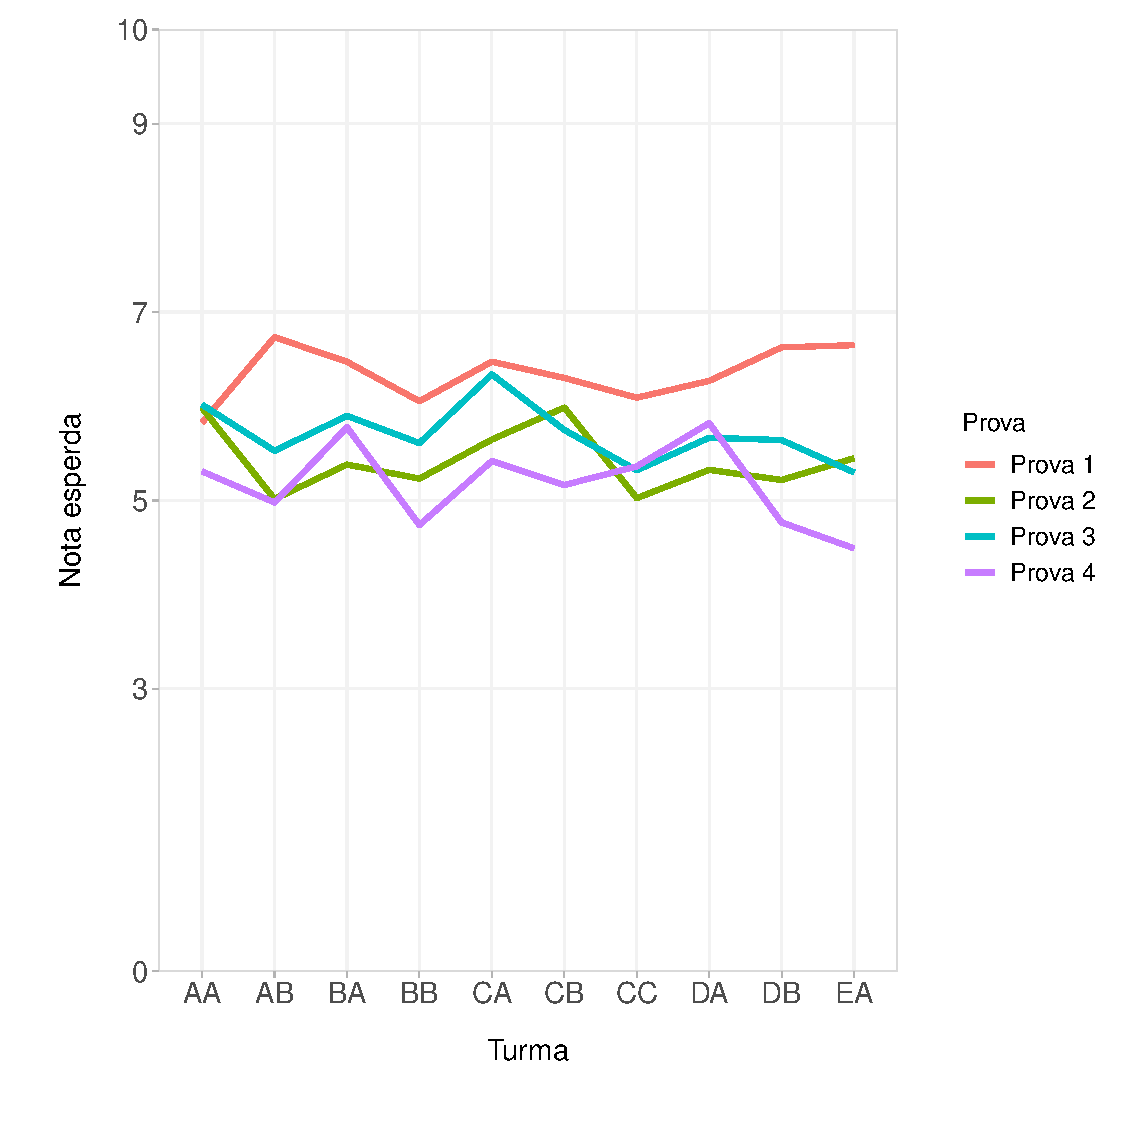
\includegraphics[width=7.5cm, height=7.5cm]{nota_esperada.pdf}}
    \subfloat[\footnotesize{Avaliação via teoria clássixa x TRI.}]{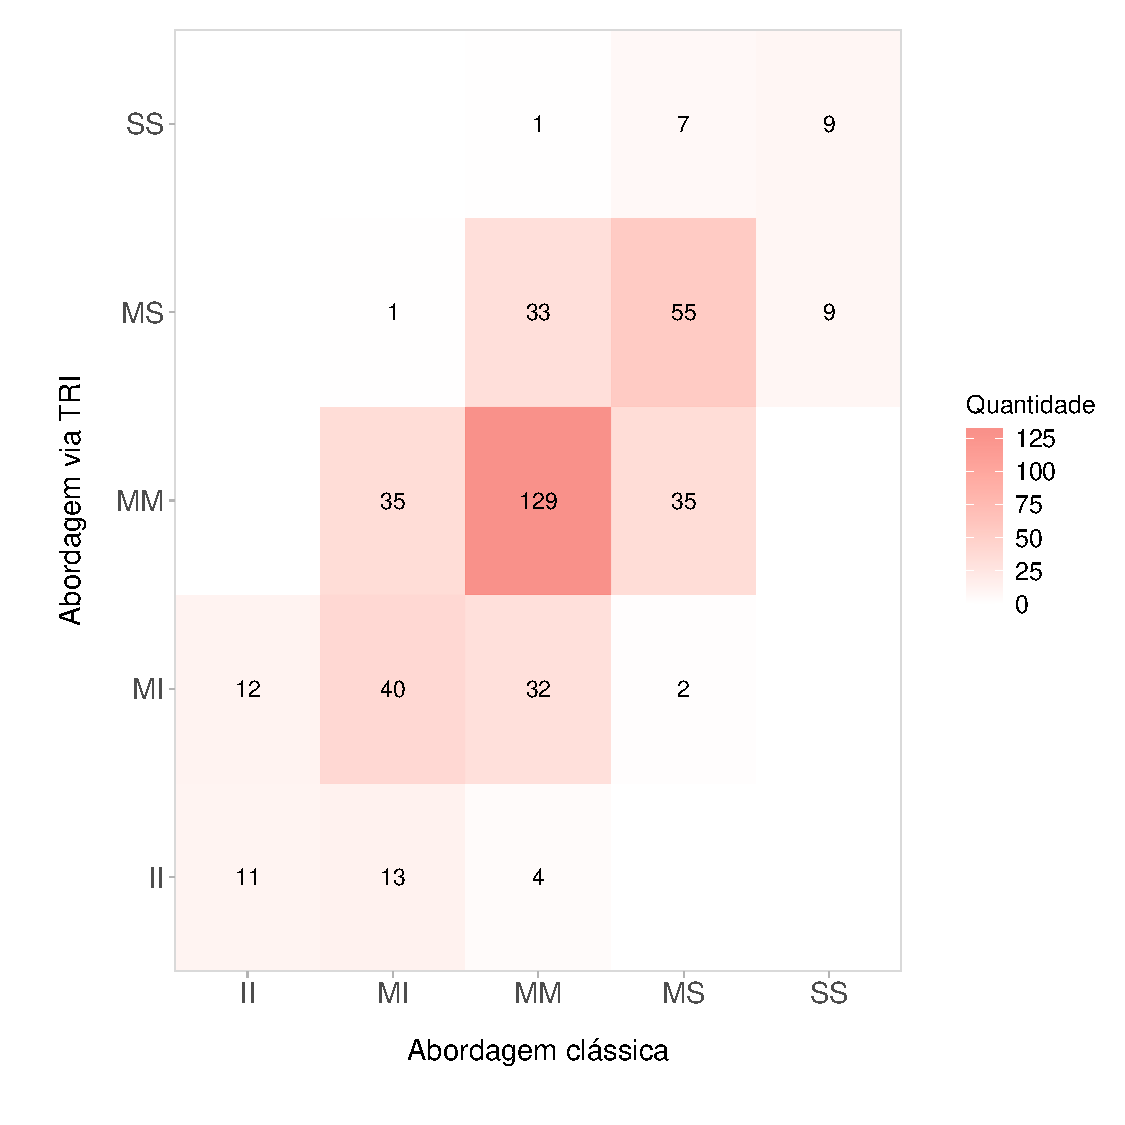
\includegraphics[width=7.5cm, height=7.5cm]{confusao_TRI.pdf}}
    \\
    \subfloat[\footnotesize{Informação do teste.}]{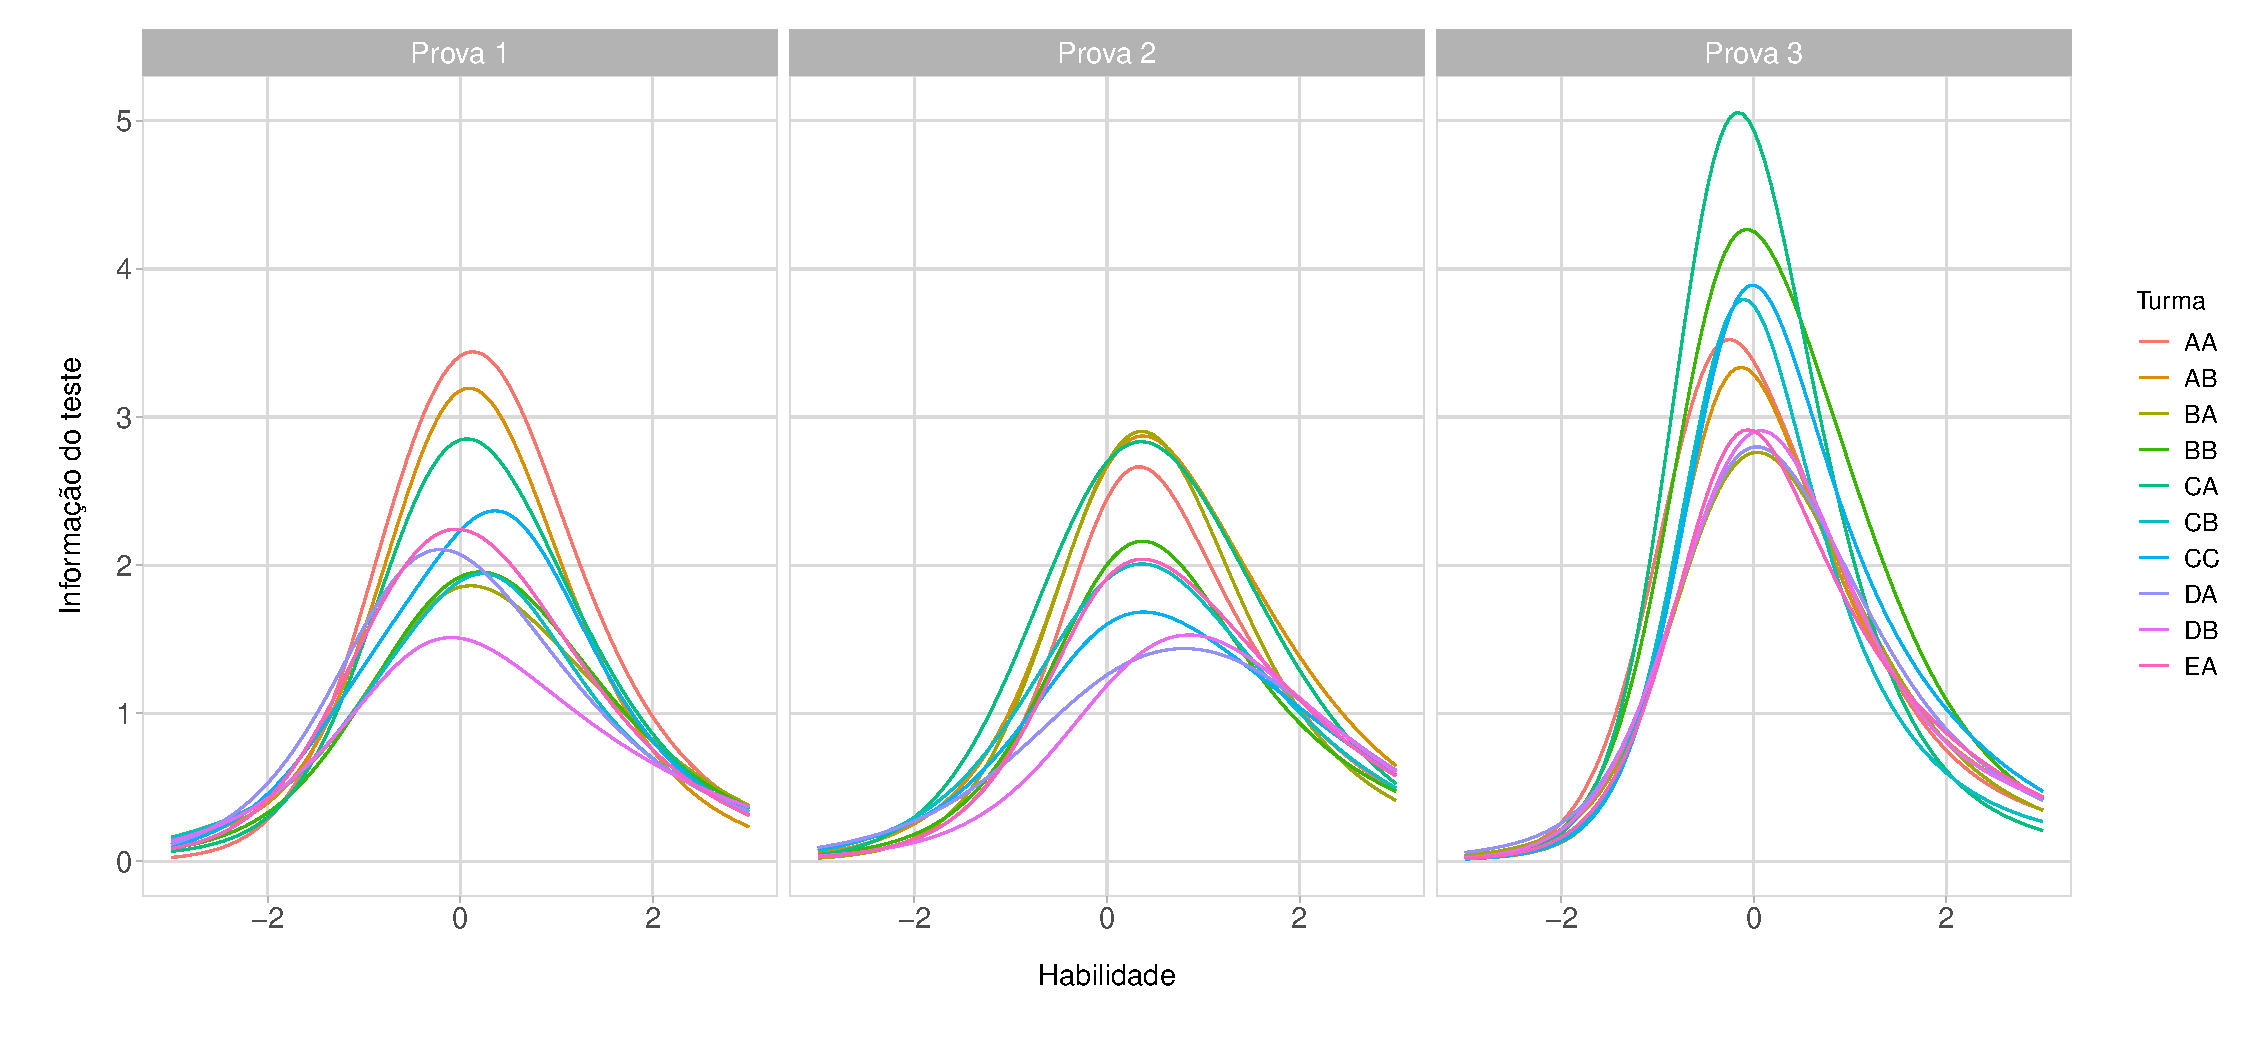
\includegraphics[width=15cm, height=7cm]{teste.inf.pdf}}
\caption{(a) Nota esperada de um aluno com habilidade mediana (isso é, com $\theta=0$). (b) Número de alunos em cada menção, calculando-a com base na nota final observada (menção real) e na habilidade final estimada via TRI (definida como a média ponderada das habilidades estimadas nas provas, usando-se os mesmos pesos e protocolos da prova substitutiva). Para as menções via TRI, ordenamos e dividimos os alunos de modo a manter os percentuais observado nas menções reais. (c) Informação do teste por turma e por número da prova.}
\label{fig:Diversos.TRI}
\end{figure}

\begin{figure} 
    \centering
  \subfloat[\footnotesize{Correlograma dos resíduos por tema.}]{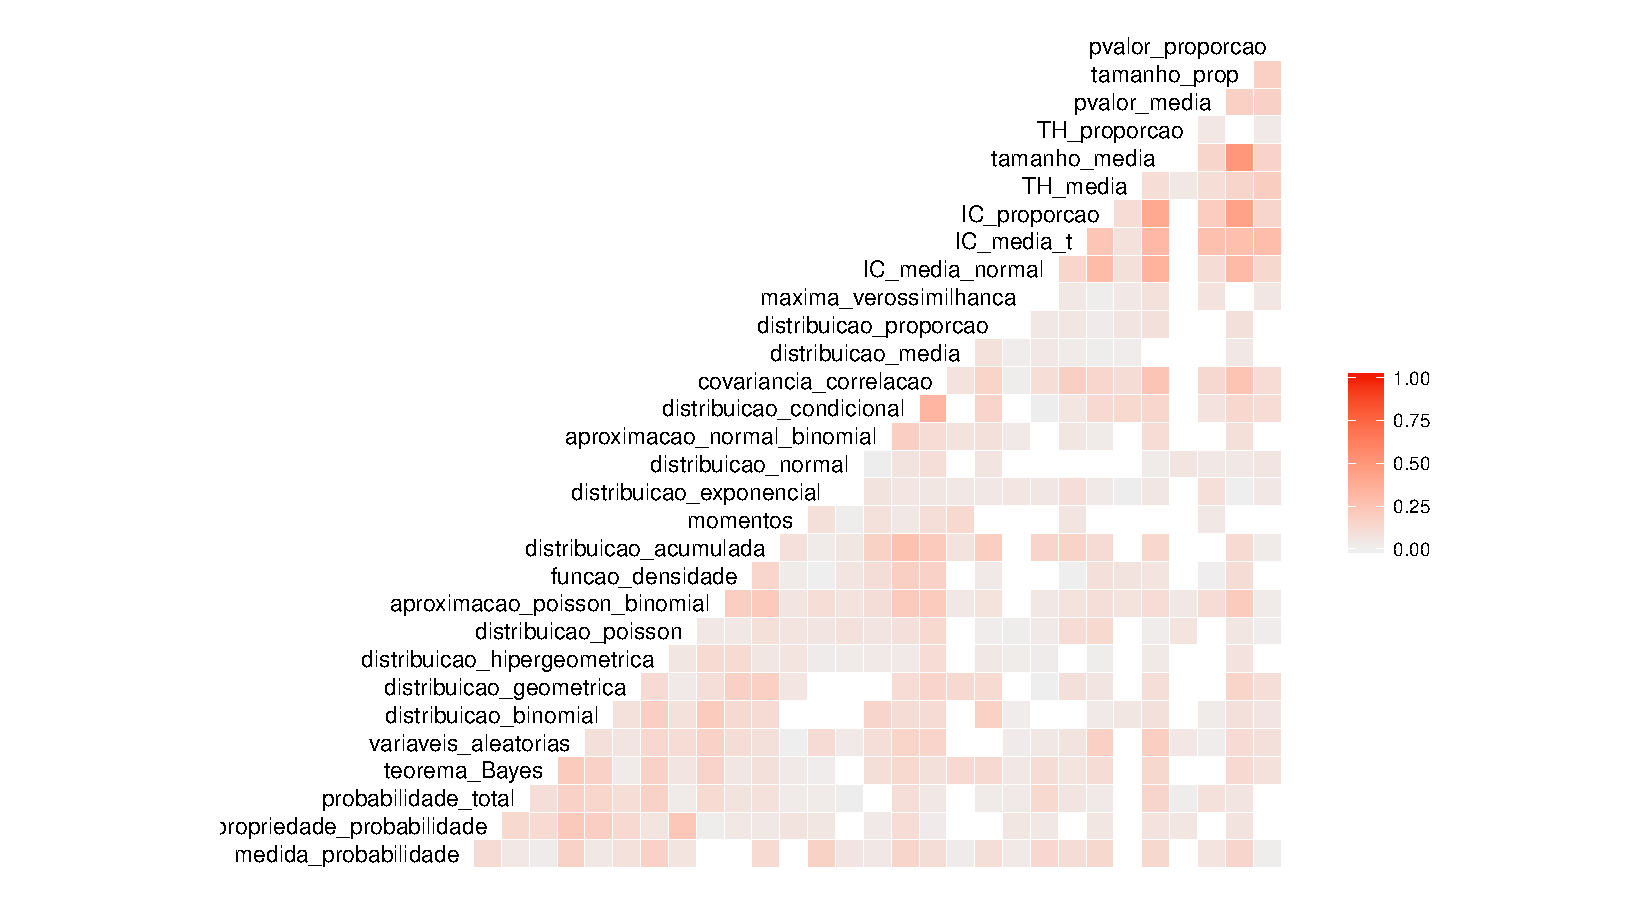
\includegraphics[width=16.5cm, height=9cm]{correlograma.pdf}}
  \\
    \subfloat[\footnotesize{Grafo de associação dos resíduos.}]{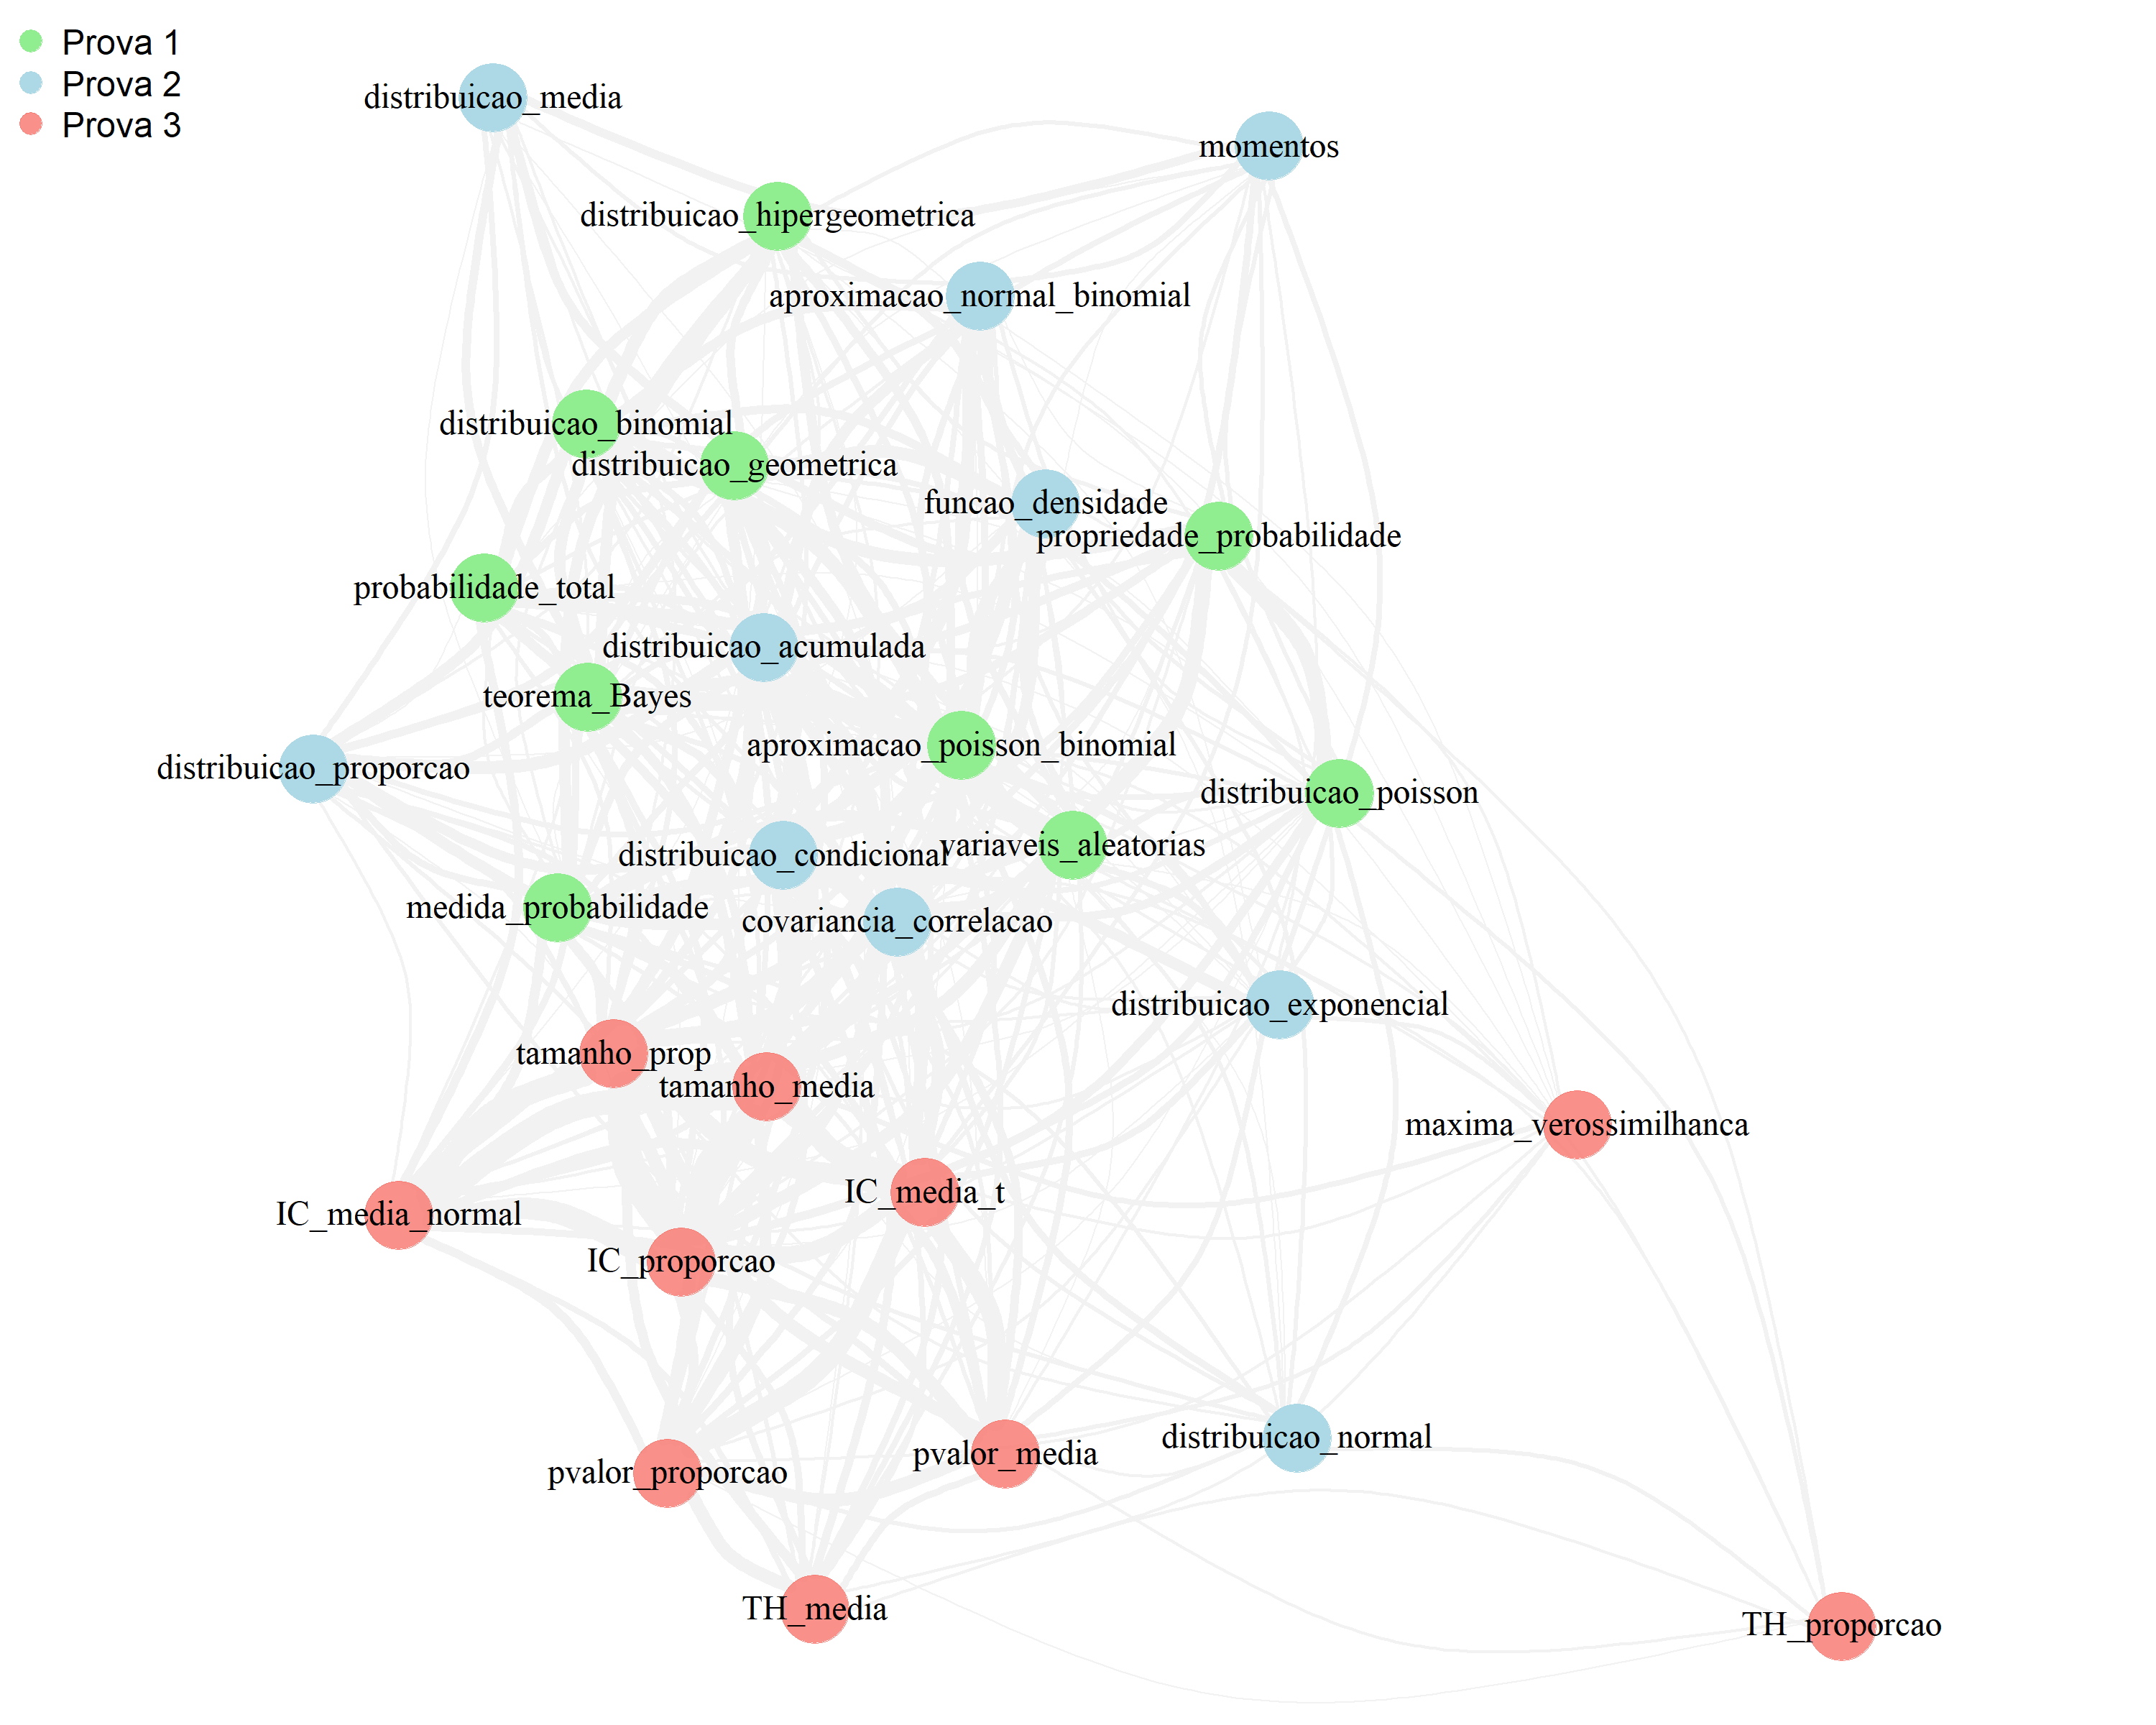
\includegraphics[width=15cm, height=12cm]{rede.png}}
\caption{(a) Correlograma (de Pearson) dos \emph{resíduos componente do desvio} (RCD) por tema. Valores negativos foram substituídos por zero. (b) Rede de associação dos resíduos por tema.}
\label{fig:Correlacao}
\end{figure}

\subsection{Avaliação das questões} \label{subsec:banco}

Nesta seção, apresentamos um estudo da qualidade das questões, de acordo
com o ajuste via TRI.

A figura 2.6 nos indica a probabilidade de um aluno mediano acertar cada
questão aplicada durante o semestre. Temas com maior variabilidade entre
as probabilidades são justamente aqueles em que os modelos de questão
são mais heterogêneos.

As questões de alguns temas são notadamente mais fáceis. Por exemplo, na
Prova 1, percebe-se que os pontos referentes ao tema
\emph{lei da probabilidade total} etão mais à direita, o que era de se
esperar. Na Prova 3, os temas mais fáceis são os que tratam de tamanho
da amostra e intervalo de confiança calculados a partir da tabela da
distribuição Normal. Nesses casos, mesmo que o aluno não entenda
plenamente os conceitos estatísticos, ele poderia acertar as questões
desde de que identificasse corretamente a formula que deveria aplicar.
Conforme visto anteriormente, o tema
\emph{Teste de hipóteses para a proporção} foi o mais difícil. Entre as
possíveis explicações está o nível de dificuldade das questões, o fato
de este ser o último tema ministrado no curso ou alguma deficiência no
processo de ensino. Os dados apresentados neste gráfico também estão
disponíveis nas tabelas do Apêndice \ref{sec:tabelas}.

As Figuras 2.7 a 2.9 representam as curvas características das questões
aplicadas nas provas 1 a 3. Quando a probabilidade de acerto do aluno
mais habilidoso (habilidade=3) é inferior a 0.8 ou a probabilidade de
acerto do aluno menos habilidoso (habilidade=-3) é superior a 0.4,
sugerimos que a questão seja revisada. Tais questões estão representadas
por linhas tracejadas. A leitura cuidadosa das cursvas características
indicam a origem do problema. Se a curva apresentar pouca variação, o
item não está fortemente associado à habilidade do aluno (o parametro
\(a\) é baixo). Se ela começar de uma posição elevada, um aluno pouco
proficiente é capaz de deduzir a resposta correta com probabilidade
alta. Por fim, quando a curva parece estar horizontalmente deslocada
para direita (esquerda), a questão é muito fácil (difícil).

Na tabela 2.2, identificamos as questões que devem ser revisadas. A
tabela completa (com todas as questões aplicadas) está disponível no
Apêndice \ref{sec:tabelas}.

\begin{figure}
\centering
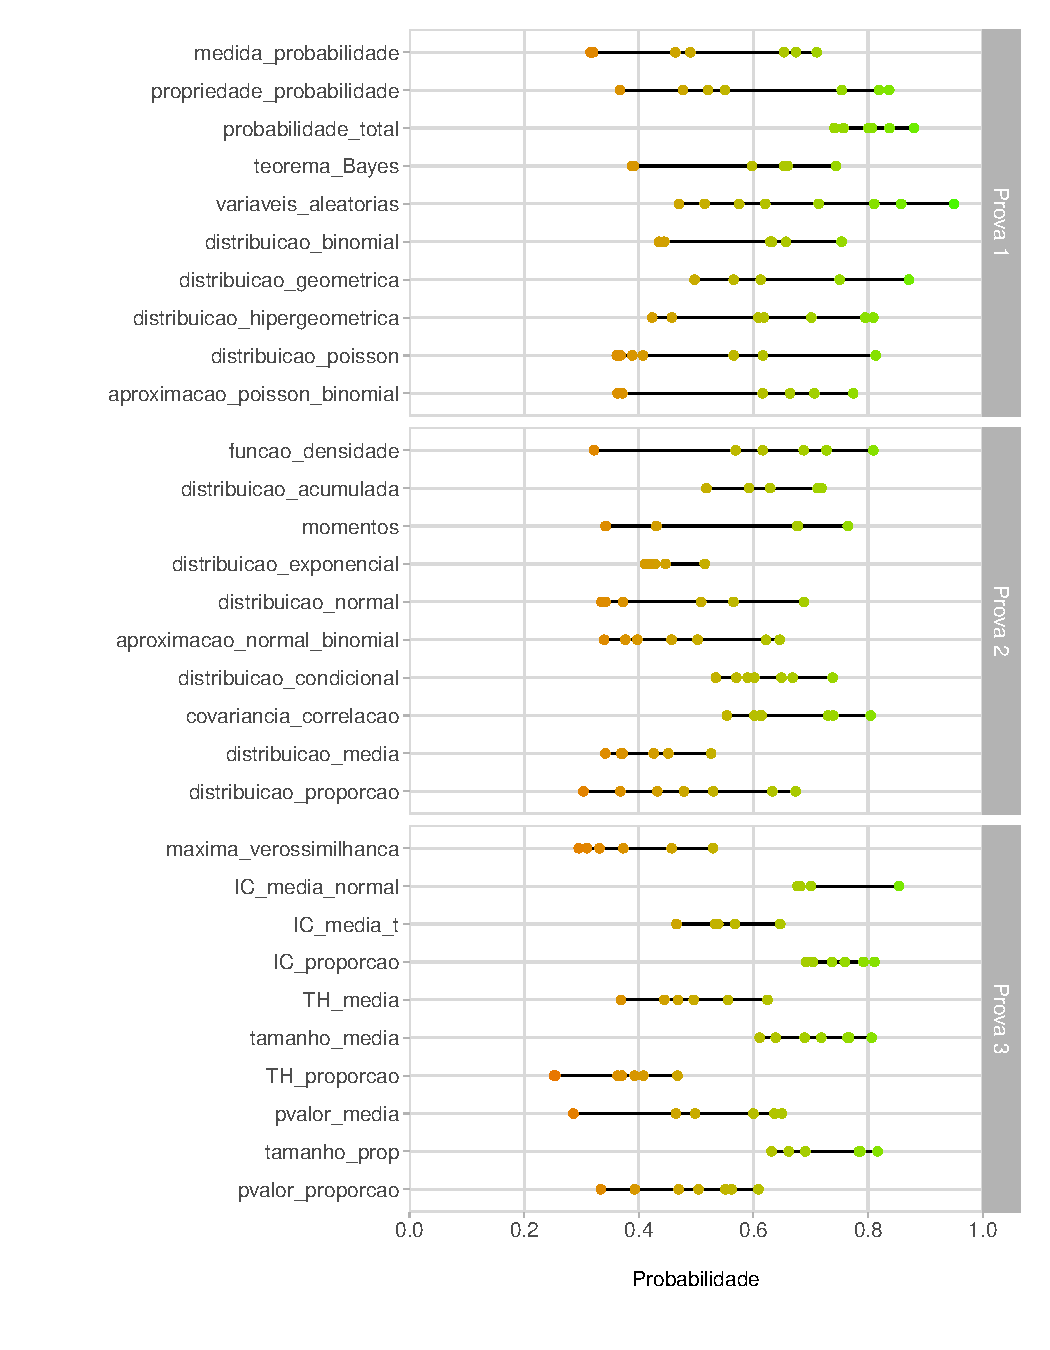
\includegraphics{Relatorio_files/figure-latex/unnamed-chunk-5-1.pdf}
\caption{Probabilidade de um aluno mediano (habilidade igual a zero)
responder corretamente cada questão do banco que tenha sido sorteada a
pelo menos uma das turmas nas provas 1 a 3.}
\end{figure}

\begin{figure}
\centering
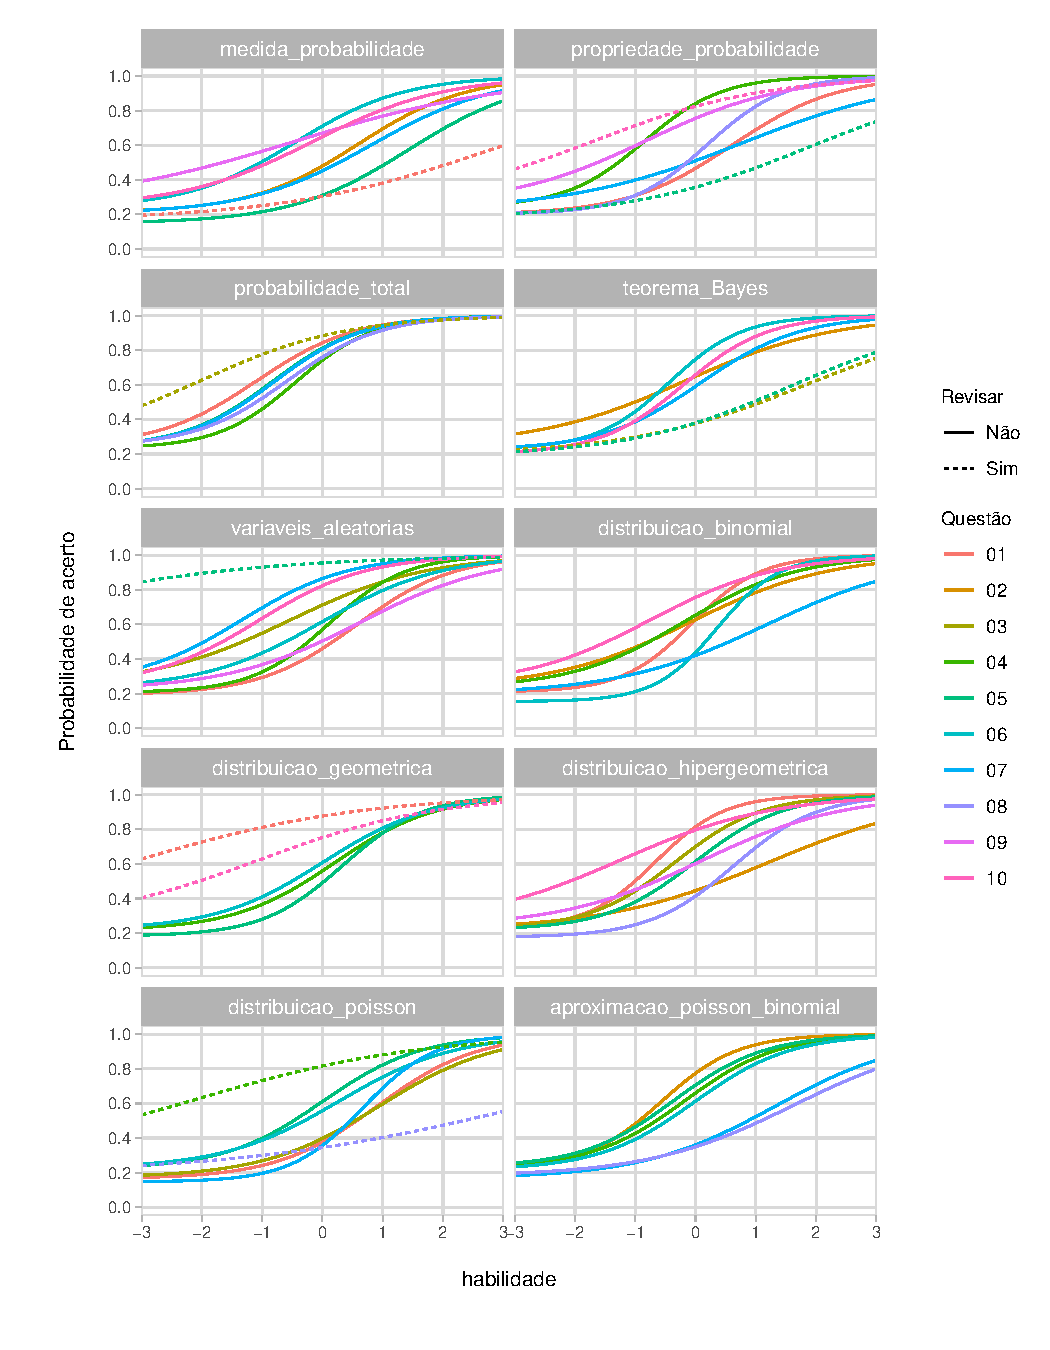
\includegraphics{Relatorio_files/figure-latex/unnamed-chunk-6-1.pdf}
\caption{Curva característica dos itens (indica a probabilidade de um
aluno com dada habilidade acertar ao respectivo item) da Prova 1.}
\end{figure}

\begin{figure}
\centering
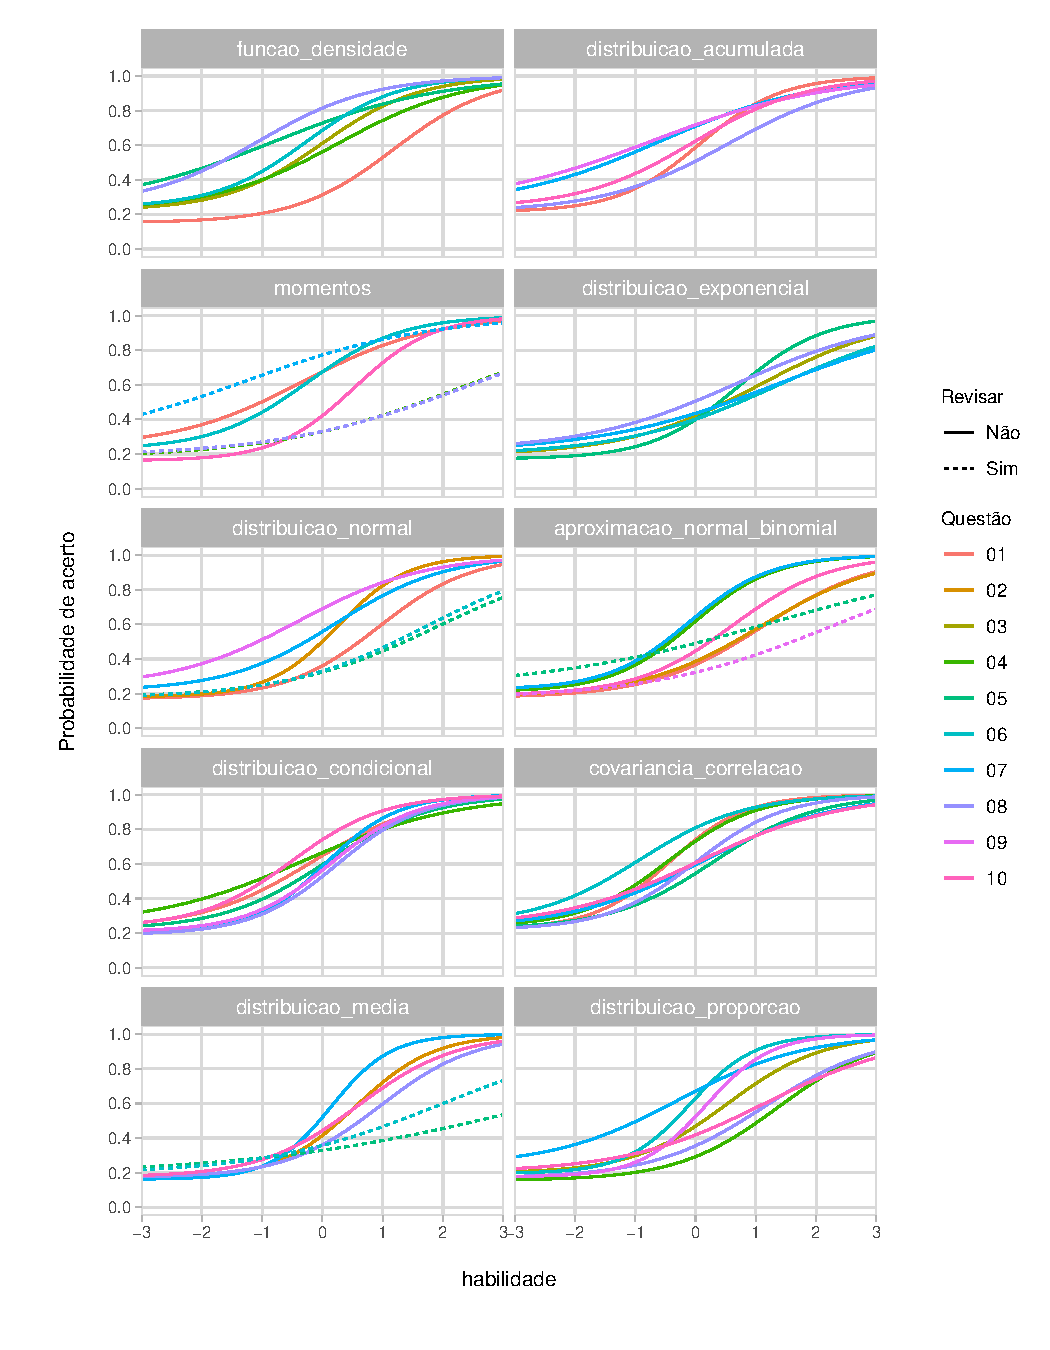
\includegraphics{Relatorio_files/figure-latex/unnamed-chunk-7-1.pdf}
\caption{Curva característica dos itens (indica a probabilidade de um
aluno com dada habilidade acertar ao respectivo item) da Prova 2.}
\end{figure}

\begin{figure}
\centering
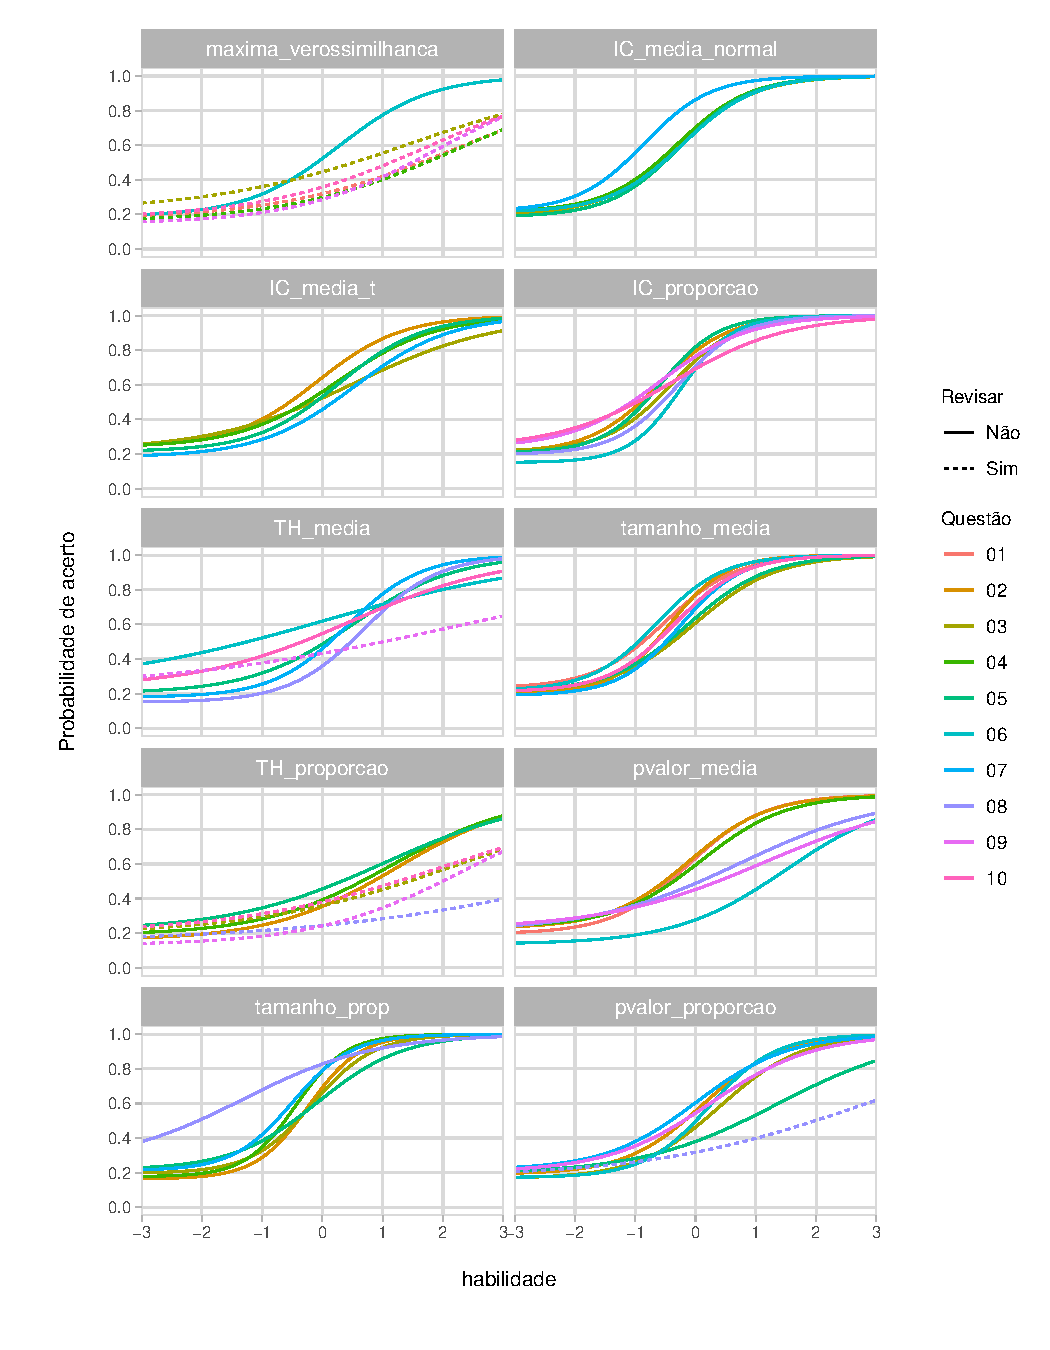
\includegraphics{Relatorio_files/figure-latex/unnamed-chunk-8-1.pdf}
\caption{Curva característica dos itens (indica a probabilidade de um
aluno com dada habilidade acertar ao respectivo item) da Prova 3.}
\end{figure}

\newpage

\begin{longtable}{l|c|c|c|c|c|c|c|c|c}
\caption{\label{tab:unnamed-chunk-9}Parâmetros das questão a revisar.  
      n:número de respondentes; p1, p2 e p3: probabilidade de acerto de um aluno com habilidade -3 (mínima), 0 (mediana) e 3 (máxima).}\\
\hline
Tema & Q & a & b & c & n & \% acerto & p1 & p2 & p3\\
\hline
\endfirsthead
\caption[]{Parâmetros das questão a revisar  (continuação)}\\
\hline
Tema & Q & a & b & c & n & \% acerto & p1 & p2 & p3\\
\hline
\endhead
medida\_probabilidade & 01 & 0.6 & 1.6 & 0.17 & 44 & 27 & 20 & 32 & 60\\
\hline
propriedade\_probabilidade & 05 & 0.7 & 1.3 & 0.18 & 90 & 37 & 21 & 37 & 74\\
\hline
propriedade\_probabilidade & 10 & 0.7 & -1.2 & 0.25 & 39 & 85 & 46 & 82 & 97\\
\hline
probabilidade\_total & 03 & 0.8 & -1.7 & 0.25 & 132 & 87 & 48 & 88 & 99\\
\hline
teorema\_Bayes & 03 & 0.7 & 1.3 & 0.20 & 89 & 38 & 23 & 39 & 75\\
\hline
teorema\_Bayes & 05 & 0.7 & 1.2 & 0.19 & 45 & 38 & 21 & 39 & 79\\
\hline
variaveis\_aleatorias & 05 & 0.5 & -2.7 & 0.27 & 52 & 100 & 84 & 95 & 99\\
\hline
distribuicao\_geometrica & 01 & 0.5 & -1.6 & 0.26 & 48 & 90 & 63 & 87 & 97\\
\hline
distribuicao\_geometrica & 10 & 0.7 & -0.7 & 0.24 & 44 & 77 & 40 & 75 & 95\\
\hline
distribuicao\_poisson & 04 & 0.5 & -1.1 & 0.25 & 48 & 83 & 53 & 81 & 96\\
\hline
distribuicao\_poisson & 08 & 0.4 & 1.4 & 0.19 & 16 & 25 & 24 & 36 & 55\\
\hline
momentos & 04 & 0.6 & 1.5 & 0.18 & 44 & 30 & 20 & 34 & 67\\
\hline
momentos & 07 & 0.7 & -0.8 & 0.25 & 16 & 81 & 43 & 76 & 96\\
\hline
momentos & 08 & 0.6 & 1.5 & 0.19 & 96 & 34 & 21 & 34 & 67\\
\hline
distribuicao\_normal & 05 & 0.8 & 1.5 & 0.18 & 133 & 34 & 19 & 33 & 76\\
\hline
distribuicao\_normal & 06 & 0.9 & 1.5 & 0.18 & 94 & 33 & 19 & 34 & 79\\
\hline
aproximacao\_normal\_binomial & 05 & 0.5 & 0.7 & 0.23 & 63 & 51 & 30 & 50 & 77\\
\hline
aproximacao\_normal\_binomial & 09 & 0.7 & 1.5 & 0.17 & 14 & 14 & 20 & 34 & 69\\
\hline
distribuicao\_media & 05 & 0.4 & 1.5 & 0.19 & 88 & 32 & 23 & 34 & 54\\
\hline
distribuicao\_media & 06 & 0.7 & 1.3 & 0.19 & 111 & 37 & 22 & 37 & 73\\
\hline
maxima\_verossimilhanca & 01 & 0.7 & 1.5 & 0.17 & 48 & 29 & 19 & 33 & 69\\
\hline
maxima\_verossimilhanca & 03 & 0.6 & 0.9 & 0.22 & 141 & 46 & 27 & 46 & 78\\
\hline
maxima\_verossimilhanca & 04 & 0.7 & 1.6 & 0.16 & 47 & 28 & 18 & 31 & 69\\
\hline
maxima\_verossimilhanca & 09 & 0.9 & 1.6 & 0.15 & 84 & 30 & 16 & 30 & 76\\
\hline
maxima\_verossimilhanca & 10 & 0.7 & 1.3 & 0.18 & 16 & 25 & 20 & 37 & 77\\
\hline
TH\_media & 09 & 0.4 & 1.0 & 0.22 & 178 & 44 & 30 & 44 & 65\\
\hline
TH\_proporcao & 03 & 0.6 & 1.4 & 0.19 & 131 & 37 & 23 & 37 & 69\\
\hline
TH\_proporcao & 08 & 0.4 & 2.1 & 0.15 & 48 & 19 & 18 & 25 & 40\\
\hline
TH\_proporcao & 09 & 0.8 & 1.9 & 0.13 & 38 & 16 & 14 & 25 & 67\\
\hline
TH\_proporcao & 10 & 0.6 & 1.2 & 0.20 & 51 & 39 & 24 & 39 & 70\\
\hline
pvalor\_proporcao & 08 & 0.6 & 1.6 & 0.18 & 16 & 19 & 20 & 33 & 62\\
\hline
\end{longtable}

\section{Conclusões, recomendações e trabalhos futuros} \label{sec:conclusao}

Neste capítulo investigamos em detalhes o desempenho dos alunos e a
qualidade das questões criadas nesse projeto. Para tanto, usamos a
Teoria de Resposta ao item, o que, no limite do nosso conhecimento,
ainda não havia sido empregada para auxiliar a gestão do processo
avaliativo em cursos oferecidos pela UnB.

O percentual de aprovação está compatível com o observado historicamente
em disciplinas em cursos de Ciências Exatas. A variação entre turmas,
por sua vez, teve uma redução substancial depois da unificação do curso
(a análise dos dados históricos poderá ser oportunamente incluída nesse
relatório).

O percentual de alunos com menção máxima, SS, sem considerar possíveis
ajustes ou arredondamentos, se mostrou demasiadamente baixo, o que
sugere a adoção de medidas que o aumentem.

Ao avaliar os dados da prova substitutiva, observamos que 78.3\(\%\) dos
alunos que a fizeram estavam reprovados. Destes, 41.7\(\%\) lograram
aprovação. Apenas 1 aluno conseguiu chegar ao SS após a prova
substitutiva.

Independentemente do método de avaliação (clássico ou via TRI), é
preciso considerar o componente aleatório dos testes. A título de
ilustração, um aluno com 8.8, submetido a outra prova, poderia, por mero
acaso, alcançar 9.2.

Apresentamos gráficos que permitem ao professor identificar temas em que
os alunos tiveram desempenho deficitário. Tal informação é útil para o
planejamento do curso no próximo semestre.

Os dados indicam que, pelo procedimento de sorteio das questões para as
turmas, as provas estão bem equilibradas em relação ao nível de
dificuldade, mas não quanto ao nível de \emph{informação}. Nesse
sentido, sugerimos que se sorteie as questões de modo que o nível de
informação dos testes seja parecido em todas as turmas.

Conforme detalhado na subseção \ref{subsec:banco}, diversas questões
deverão ser revisadas, seja por estarem descalibradas no nível de
dificuldade, por serem pouco informativas ou por conterem alternativas
falsas facilmente detectáveis.

A análise via TRI pode ser aprimorada de diversas maneiras. Por exemplo,
ao invés de considerar um modelo independente por prova, seria
preferível ajustar um único modelo capaz de acomodar a natureza temporal
dos dados. Canalizar a distribuição a posteriori dos parâmetros das
questões do semestre anterior para especificar a priori dos parâmetros
no semestre corrente traria ganhos ao modelo. Em outras palavras, se em
um dado semestre constatarmos que determinado item é difícil, devemos
nos valer dessa informação para melhorar a precisão de nossas
inferências.

\newpage

\BgThispage
\chapter{Manual de procedimentos} \label{cap:Manual}

\newpage

Este capítulo descreve o passo-a-passo necessário para gerar e corrigir
provas de uma disciplina utilizando o sistema elaborado. Este foi
desenvolvido para uso no Windows, e NÃO funciona no macOS. Para usá-las
em outro sistema operacional, é preciso editar os códigos R. Para
correta utilização do produto, é necessário que o usuário tenha noções
básicas de \texttt{R}. A disciplina de Probabilidade e Estatística (PE)
será usada como referência para facilitar a exposição dos passos, mas o
sistema também pode ser aplicado a outras disciplinas, conforme
detalhado nas próximas seções.

\section{Pré-requisitos} \label{sec:requisitos}

Os pré-requisitos necessários para utilização do sistema estão descritos
a seguir.

\subsection{Programas}

Para executar os códigos será necessária a instalação dos seguintes
programas (todos de livre acesso):

\begin{itemize}
\tightlist
\item
  RStudio (versão utilizada: 3.5.1);
\item
  Pacote R exams (versão utilizada: 2.3-2);
\item
  wkhtmltopdf (versão utilizada: 0.12.5);
\item
  Rtools (versão utilizada: Rtools version 3.5.0.4. Na instalação,
  marcar a caixa ``add app directory to the system path'');
\item
  PDFTk (versão utilizada: 2.0.2);
\item
  GhostScript (versão utilizada: 9.50);
\item
  ImageMagick's convert (com a opção legacy convert.exe). Veja a Seção
  ``Details'' do help da função \emph{nops\_scan()} do \texttt{R}.
\end{itemize}

\subsection{Pastas e arquivos}

Para facilitar a apresentação do sistema e auxiliar a organização dos
arquivos, é necessário criar algumas pastas no computador. Este manual
utilizará a disciplina Probabilidade e Estatística (PE) como referência,
portanto uma pasta chamada ``PE'' será criada, contendo as seguintes
subpastas:

\begin{enumerate}
\def\labelenumi{\roman{enumi}.}
\tightlist
\item
  Banco\_questoes
\item
  Suplementos
\item
  Prova\_1

  \begin{itemize}
  \tightlist
  \item
    Cadastro dos alunos
  \end{itemize}
\end{enumerate}

A seguir tem-se a descrição do conteúdo necessário em cada uma das
subpastas citadas acima.

\begin{enumerate}
\def\labelenumi{\roman{enumi}.}
\item
  A pasta ``Banco\_questoes'' deve conter as questões do banco em
  formato .Rnw e a planilha das respectivas dificuldades
  ``matriz.dificuldades.csv'' (mais detalhes desta planilha na seção
  1.2.4).
\item
  A pasta ``Suplementos'' deve conter os seguintes arquivos:
\end{enumerate}

\begin{itemize}
\tightlist
\item
  ``info.tex'' (arquivo \emph{.tex} com as instruções impressas na
  contracapa da prova).
\item
  ``Funcoes\_Extras.R'' (arquivo contendo as funções que complementam o
  pacote \emph{exams}).
\item
  ``Folha\_branco.pdf'' (arquivo pdf com apenas uma folha em branco).
\end{itemize}

\begin{enumerate}
\def\labelenumi{\roman{enumi}.}
\setcounter{enumi}{2}
\tightlist
\item
  Além disso, a pasta ``Prova\_1'' deve conter os seguintes arquivos:
\end{enumerate}

\begin{itemize}
\tightlist
\item
  gerar\_prova.R: arquivo utilizado na geração das provas.
\item
  corrigir\_prova.R : arquivo utilizado na correção das provas.
\item
  README - P1.txt : arquivo de registro dos acontecimentos relevantes
  durante o processo de correção das provas.
\item
  Para gerar as provas da disciplina de Probabilidade e Estatística (PE)
  na UnB, a pasta ``Cadastro dos alunos'' deve conter 2 arquivos com os
  dados atuais dos alunos matriculados em PE:

  \begin{itemize}
  \tightlist
  \item
    ``Composição de Turmas PE.txt'': solicitar à secretaria do
    departamento.
  \item
    ``PE.txt'': solicitar à secretaria do departamento.\\
    Além disso, a pasta ``Cadastro dos alunos'' deve conter o dicionário
    de códigos de cursos, que não precisa ser atualizado semestralmente.
  \item
    ``Código de opçoes de curso.txt''.\\
    Observação: Para gerar provas em outras instituições, a pasta
    ``Cadastro dos alunos'' pode ficar em branco nesse momento.
    \red{Atenção!} Os 3 arquivos devem estar salvos com o encoding
    UTF-8.
  \end{itemize}
\end{itemize}

Segue ilustração da organização das pastas:

\begin{figure}
\centering
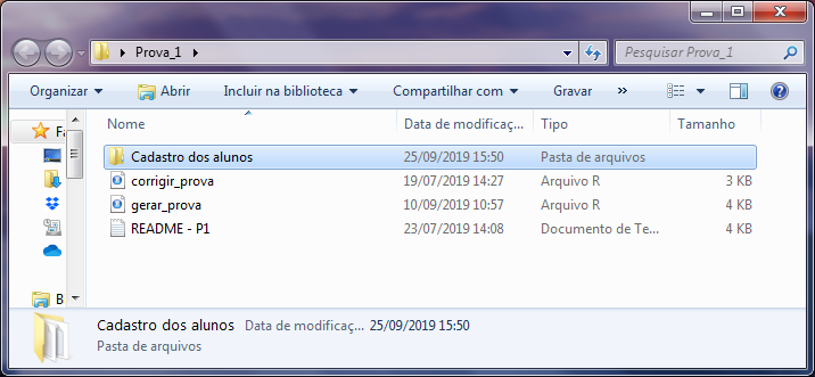
\includegraphics{imagens/pasta_prova1.png}
\caption{Ilustração da pasta ``Prova\_1''.}
\end{figure}

\begin{figure}
\centering
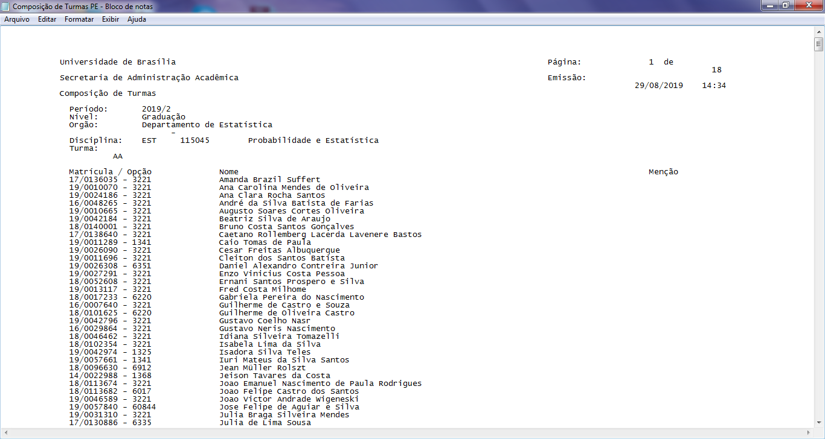
\includegraphics{imagens/arquivo_compturmas.png}
\caption{Ilustração do arquivo ``Composição de Turmas PE.txt''.}
\end{figure}

\begin{figure}
\centering
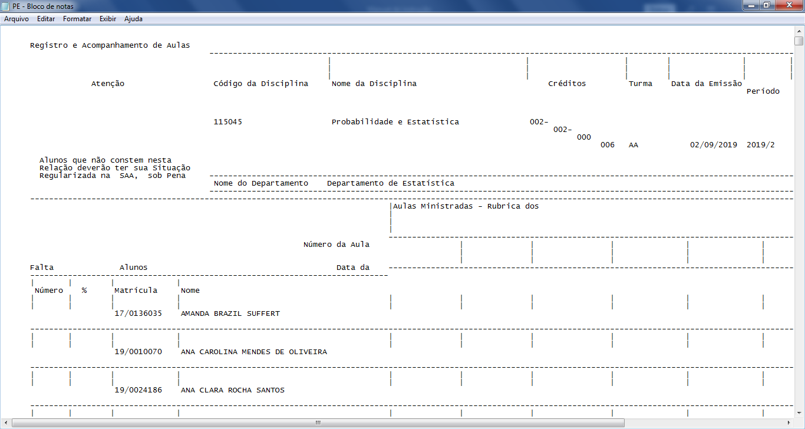
\includegraphics{imagens/pe.png}
\caption{Ilustração do arquivo ``PE.txt''.}
\end{figure}

\begin{figure}
\centering
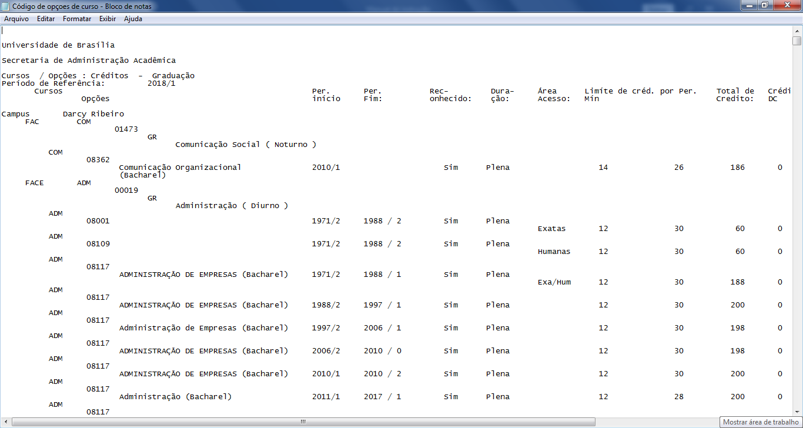
\includegraphics{imagens/arquivo_opcaocurso.png}
\caption{Ilustração do arquivo ``Código de opçoes de curso.txt''.}
\end{figure}

\begin{figure}
\centering
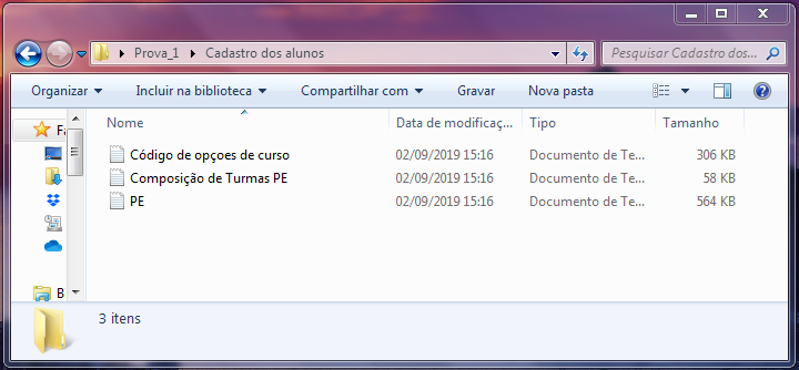
\includegraphics{imagens/pasta_cadastroaluno.png}
\caption{Ilustração da pasta ``Cadastro dos alunos'' antes do processo
de geração das provas.}
\end{figure}

\section{Geração das provas}

Após concluir a etapa de pré-requisitos, o código \emph{gerar\_prova.R}
pode ser executado conforme descrito a seguir.

\subsection{Localizando as pastas}

Execute as seguintes linhas do programa:

\begin{Shaded}
\begin{Highlighting}[]
\NormalTok{### Identificando as pastas necessárias}
\ControlFlowTok{if}\NormalTok{(}\KeywordTok{length}\NormalTok{(}\KeywordTok{ls}\NormalTok{()) }\OperatorTok{>}\StringTok{ }\DecValTok{0}\NormalTok{) }\KeywordTok{rm}\NormalTok{(}\DataTypeTok{list =} \KeywordTok{ls}\NormalTok{()) }\CommentTok{# Limpando a área de trabalho}
\NormalTok{pasta.cadastros <-}\StringTok{ }\KeywordTok{choose.dir}\NormalTok{(}\DataTypeTok{default=}\KeywordTok{getwd}\NormalTok{(), }
                              \DataTypeTok{caption=}\StringTok{"Escolha a pasta com os dados dos alunos"}\NormalTok{)}
\NormalTok{pasta.provas <-}\StringTok{ }\KeywordTok{choose.dir}\NormalTok{(}\DataTypeTok{default=}\KeywordTok{getwd}\NormalTok{(), }
                           \DataTypeTok{caption=}\StringTok{"Escolha a pasta onde salvar as provas"}\NormalTok{)}
\NormalTok{pasta.questoes <-}\StringTok{ }\KeywordTok{choose.dir}\NormalTok{(}\DataTypeTok{default=}\KeywordTok{getwd}\NormalTok{(), }
                             \DataTypeTok{caption=}\StringTok{"Escolha a pasta com o banco de questoes"}\NormalTok{)}
\NormalTok{pasta.suplementos <-}\StringTok{ }\KeywordTok{choose.dir}\NormalTok{(}\DataTypeTok{default=}\KeywordTok{getwd}\NormalTok{(), }
                              \DataTypeTok{caption=}\StringTok{"Escolha a pasta com os arquivos suplementares"}\NormalTok{)}
\end{Highlighting}
\end{Shaded}

Nesse passo, o programa solicitará que o usuário indique a localização
de alguns arquivos. Mais especificamente, quatro pastas precisam ser
especificadas, conforme exemplificado abaixo:

\begin{itemize}
\tightlist
\item
  Escolha a pasta com os dados dos alunos:
  \textbackslash{}PE\textbackslash{}Prova\_1\textbackslash{}Cadastro dos
  alunos.
\item
  Escolha a pasta onde salvar as provas:
  \textbackslash{}PE\textbackslash{}Prova\_1.
\item
  Escolha a pasta com o banco de questões:
  \textbackslash{}PE\textbackslash{}Banco\_questoes.
\item
  Escolha a pasta com os arquivos suplementares:
  \textbackslash{}PE\textbackslash{}Suplementos.
\end{itemize}

\subsection{Carregando as funções suplementares}

Execute a seguinte linha do programa:

\begin{Shaded}
\begin{Highlighting}[]
\NormalTok{### Carregando as funcoes suplementares usadas no codigo}
\KeywordTok{source}\NormalTok{(}\KeywordTok{paste0}\NormalTok{(pasta.suplementos, }\StringTok{"}\CharTok{\textbackslash{}\textbackslash{}}\StringTok{Funcoes_Extras.R"}\NormalTok{))  }\CommentTok{# Complementando pacote Exams }
\end{Highlighting}
\end{Shaded}

Além da estrutura presente no pacote \emph{exams}, outras funções foram
desenvolvidas para complementar o sistema de avaliação. Nessa etapa,
essas funções extras serão carregadas no R.

\subsection{Organizando o cadastro dos alunos}

Aqui, o programa cria o cadastro dos alunos com base nos arquivos
disponibilizados pela secretaria do departamento de Estatística da
Universidade de Brasília. Em outras instituições, o usuário não precisa
rodar essa seção (leia a observação de como proceder no final desse
tópico).

\begin{Shaded}
\begin{Highlighting}[]
\NormalTok{### Organizando o cadastro a partir dos arquivos disponibilizados pela secretaria.}
\NormalTok{cadastro <-}\StringTok{ }\KeywordTok{gerar.cadastro}\NormalTok{() }\CommentTok{# Gerando um arquivo csv com o cadastro.}
\end{Highlighting}
\end{Shaded}

Nesse passo, o programa solicitará que o usuário indique a localização
dos seguintes arquivos:

\begin{itemize}
\tightlist
\item
  Arquivo .txt com os dados dos alunos: ``PE.txt''.
\item
  Arquivo .txt com os dados dos cursos dos alunos: ``Composição de
  Turmas PE.txt''.
\item
  Arquivo .txt com o dicionário de códigos de cursos: ``Código de opçoes
  de curso.txt''.
\end{itemize}

O comando acima irá incluir automaticamente na pasta ``Cadastro dos
alunos'' uma planilha de alunos matriculados para cada turma e uma
planilha contendo informação de todas as turmas, conforme ilustrado a
seguir.

\begin{figure}
\centering
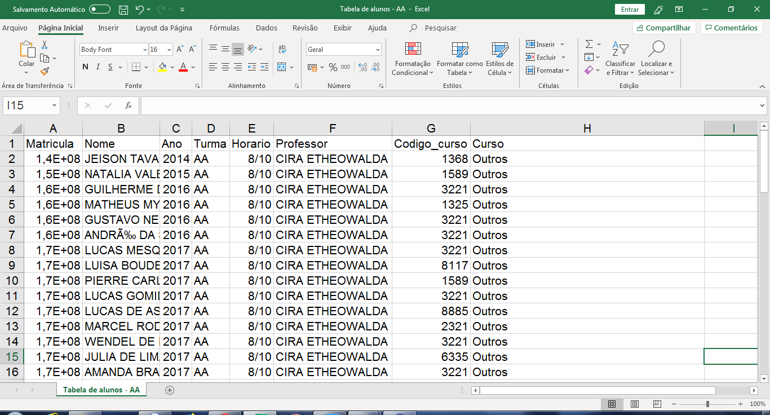
\includegraphics{imagens/arquivo_cadastro.png}
\caption{Ilustração do arquivo ``Tabela de alunos matriculados.csv''.}
\end{figure}

Observação: Para geração de provas em outras universidades, não é
necessário rodar essa seção. No entanto, será necessário incluir na
pasta ``Cadastro dos alunos'' as planilhas por turma ``Tabela de alunos
-- XX.csv'' seguindo o modelo acima e exatamente essa nomenclatura dos
arquivos. Além disso, deve-se combinar os dados de todas as turmas na
``Tabela de alunos matriculados.csv'' seguindo o mesmo modelo. A pasta
``Cadastro dos alunos'' deve conter os arquivos \emph{.csv} ilustrados
na figura a seguir (e os arquivos .txt para o caso de PE). Novamente,
lembre-se de salvar os arquivos usando o encoding UTF-8.

\begin{figure}
\centering
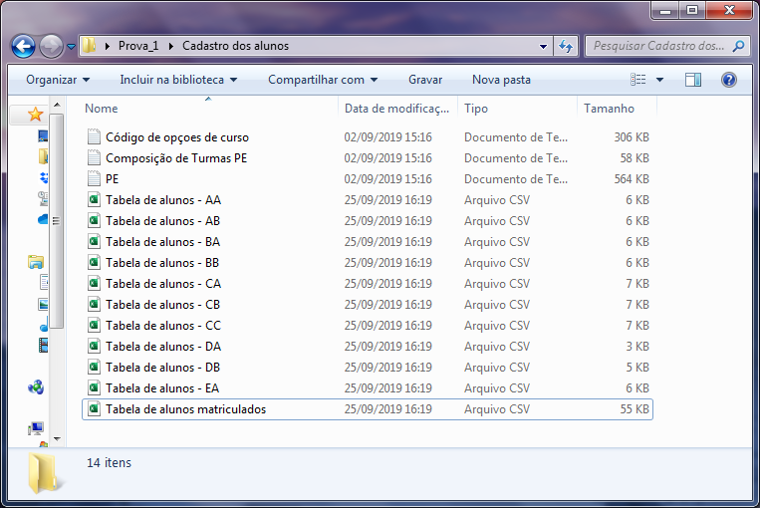
\includegraphics{imagens/pasta_cadastroaluno2.png}
\caption{Ilustração da pasta ``Cadastro dos alunos''.}
\end{figure}

\subsection{Definindo os parâmetros da prova}

Execute o código a seguir alterando os parâmetros conforme as
respectivas informações da prova.

\begin{Shaded}
\begin{Highlighting}[]
\NormalTok{### Definindo os parâmetros da prova}
\NormalTok{semente <-}\StringTok{ }\DecValTok{8768435}  \CommentTok{# Por segurança, trocar esse número a cada aplicação}
\KeywordTok{set.seed}\NormalTok{(semente)  }\CommentTok{# Definindo a semente do algoritmo}
\NormalTok{numero.prova <-}\StringTok{ }\DecValTok{1}  \CommentTok{# Número da prova}
\NormalTok{nome.prova <-}\StringTok{ }\KeywordTok{paste0}\NormalTok{(}\StringTok{"Prova_"}\NormalTok{, numero.prova)  }\CommentTok{# Nome da prova}
\NormalTok{titulo.prova <-}\StringTok{ }\KeywordTok{paste}\NormalTok{(}\StringTok{"Prova"}\NormalTok{, numero.prova)  }\CommentTok{# Titulo incluído na folha de respostas}
\NormalTok{data.prova <-}\StringTok{ "2019-09-18"}  \CommentTok{# aaaa-mm-dd}
\NormalTok{n.questoes <-}\StringTok{ }\DecValTok{10}  \CommentTok{# Definindo o número de questões na prova }
\NormalTok{total.pontos <-}\StringTok{ }\DecValTok{10}   \CommentTok{# Definindo a pontuação máxima da prova}
\end{Highlighting}
\end{Shaded}

Aqui é essencial modificar a semente do algoritmo a cada nova aplicação
de prova. A semente é importante para garantir a reprodutividade dos
resultados ao rodar novamente o código, se for necessário. Além disso, o
uso de uma semente repetida ou previsível poderia, em casos extremos,
colocar em risco o sigilo da prova.

\subsection{Definindo os temas da prova}

O banco de questões é organizado por tema, e o nome dos arquivos seguem
a seguinte nomenclatura ``xx\_nome.tema\_yy.Rnw'', onde ``xx''
representa o número do tema e ``yy'' o número da questão do respectivo
tema. A estrutura de questões da prova é definida nesse estágio, sendo
adotada 1 questão por tema, todas com igual pontuação (a primeira
questão pode ter sua pontuação ligeiramente alterada para garantir que a
soma dos pontos seja exatamente igual ao valor previamente definido).
Alterações nesta estrutura padrão devem ser feitas com cautela.

\begin{Shaded}
\begin{Highlighting}[]
\NormalTok{### Definindo os temas da prova}
\NormalTok{aux <-}\StringTok{ }\KeywordTok{list.files}\NormalTok{(pasta.questoes, }\StringTok{".Rnw"}\NormalTok{)}
\NormalTok{banco.questoes <-}\StringTok{ }\KeywordTok{vector}\NormalTok{(n.questoes, }\DataTypeTok{mode=}\StringTok{"list"}\NormalTok{)}
\ControlFlowTok{for}\NormalTok{(questao }\ControlFlowTok{in} \DecValTok{1}\OperatorTok{:}\NormalTok{n.questoes) \{  }\CommentTok{# Uma questão por tópico}
\NormalTok{  topico <-}\StringTok{ }\KeywordTok{formatC}\NormalTok{(questao }\OperatorTok{+}\StringTok{ }\DecValTok{10}\OperatorTok{*}\NormalTok{(numero.prova }\OperatorTok{-}\StringTok{ }\DecValTok{1}\NormalTok{), }\DataTypeTok{digits=}\DecValTok{1}\NormalTok{, }\DataTypeTok{flag=}\StringTok{"0"}\NormalTok{, }\DataTypeTok{format=}\StringTok{"d"}\NormalTok{)}
\NormalTok{  banco.questoes[[questao]] <-}\StringTok{ }\NormalTok{aux[}\KeywordTok{str_detect}\NormalTok{(aux, }\KeywordTok{paste0}\NormalTok{(}\StringTok{"^"}\NormalTok{, topico))]}
\NormalTok{\}}
\end{Highlighting}
\end{Shaded}

\begin{Shaded}
\begin{Highlighting}[]
\NormalTok{### Definições padrão}
\NormalTok{aux <-}\StringTok{ }\KeywordTok{list.files}\NormalTok{(pasta.cadastros)  }\CommentTok{# Lendo os cadastros das turmas}
\NormalTok{cadastro.turmas <-}\StringTok{ }\NormalTok{aux[}\KeywordTok{grep}\NormalTok{(}\StringTok{"Tabela de alunos - "}\NormalTok{, aux)]}
\NormalTok{turmas <-}\StringTok{ }\KeywordTok{substr}\NormalTok{(cadastro.turmas, }\DecValTok{20}\NormalTok{, }\DecValTok{21}\NormalTok{)  }\CommentTok{# Identificando a sigla das turmas}
\NormalTok{n.turmas <-}\StringTok{ }\KeywordTok{length}\NormalTok{(cadastro.turmas)  }\CommentTok{# Identificando o número de turmas}
\NormalTok{n.temas <-}\StringTok{ }\KeywordTok{length}\NormalTok{(banco.questoes) }\CommentTok{# Definindo o número de temas na prova}
\NormalTok{questoes.por.tema <-}\StringTok{ }\KeywordTok{rep}\NormalTok{(}\DecValTok{1}\NormalTok{, n.questoes)  }\CommentTok{# Definindo o número de questões por tema}
\NormalTok{pontos <-}\StringTok{ }\KeywordTok{round}\NormalTok{(total.pontos}\OperatorTok{*}\KeywordTok{rep}\NormalTok{(}\DecValTok{1}\OperatorTok{/}\NormalTok{n.questoes, n.questoes), }\DecValTok{2}\NormalTok{)  }\CommentTok{# Valor da questão}
\NormalTok{pontos[}\DecValTok{1}\NormalTok{] <-}\StringTok{ }\KeywordTok{round}\NormalTok{(total.pontos}\OperatorTok{-}\KeywordTok{sum}\NormalTok{(pontos[}\OperatorTok{-}\DecValTok{1}\NormalTok{]), }\DecValTok{2}\NormalTok{)}
\end{Highlighting}
\end{Shaded}

\subsection{Sorteando as questões para as turmas} \label{subsec:sorteio}

Rode o código a seguir.

\begin{Shaded}
\begin{Highlighting}[]
\NormalTok{### Sortear as questões para as turmas}
\NormalTok{questoes.sorteadas <-}\StringTok{ }\KeywordTok{sortear.questoes}\NormalTok{()}
\end{Highlighting}
\end{Shaded}

No sorteio das questões, será necessário selecionar o arquivo com a
tabela de questões com as respectivas dificuldades
``PE\textbackslash{}Banco\_questoes\textbackslash{}2\_2019\textbackslash{}Completo\textbackslash{}matriz.dificuldades.csv''.
O arquivo contém o nome da questão, o percentual de acertos, o tamanho
da amostra para o qual o percentual foi calculado (apenas para
referência) e o número do tema da questão.

\begin{figure}
\centering
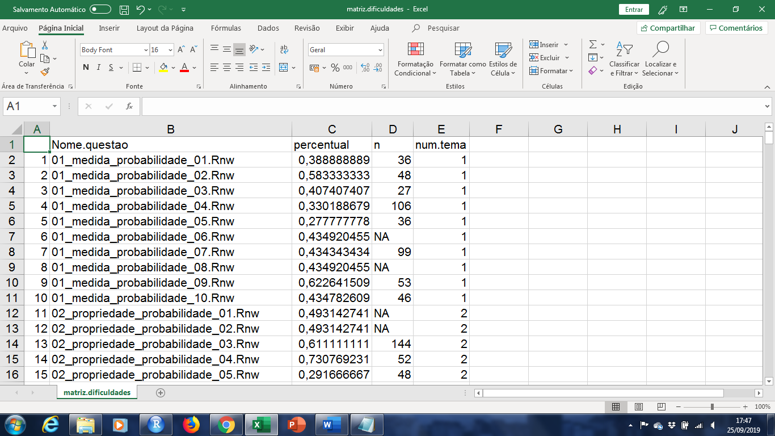
\includegraphics{imagens/arquivo_dificuldades.png}
\caption{Ilustração do arquivo ``Matriz de dificuldades.csv''.}
\end{figure}

Observação: A função ``sortear.questoes()'' tem o parâmetro
``prob.media'' que especifica a nota média desejada, com default
``prob.media=0.55''. Ao alterar essa nota, certifique-se de que as
questões do banco têm um percentual de acerto compatível. Embora esse
parâmetro possa ser usado para aumentar ou diminuir a probabilidade de
seleção de cada questão com base em seu nível de dificuldade,
recomendamos cautela na definição desse valor. Grandes alterações desse
parâmetro, para mais ou para menos, poderiam resultar em provas
desconfortavelmente parecidas entre as turmas. As questões sorteadas
serão salvas no arquivo ``Questoes\_sorteadas\_Prova\_1.csv'' na pasta
\textbackslash{}PE\textbackslash{}Prova\_1.

\subsection{Criando múltiplos exames}

Aqui as provas serão geradas para cada aluno de cada turma com base nas
questões sorteadas no passo 6. É possível adicionar uma (ou mais) página
em branco em cada prova alterando a variável ``adicionar.paginas''. Esta
página adicional pode ser usada para rascunho.

\begin{Shaded}
\begin{Highlighting}[]
\NormalTok{### criando múltiplos exames}
\KeywordTok{gerar.provas}\NormalTok{(}
  \DataTypeTok{numero.turmas=}\DecValTok{1}\OperatorTok{:}\NormalTok{n.turmas,}
  \DataTypeTok{adicionar.paginas=}\KeywordTok{rep}\NormalTok{(}\DecValTok{1}\NormalTok{, n.turmas),}
  \CommentTok{#n.provas.turmas=rep(1, n.turmas),}
  \DataTypeTok{duplex=}\NormalTok{F}
\NormalTok{)}
\end{Highlighting}
\end{Shaded}

Caso tenha interesse em testar uma versão preliminar do código, rode
essa seção desmarcando a linha\\
``\#n.provas.turmas=rep(1, n.turmas)'', fazendo com que apenas uma prova
seja gerada em cada turma.\\
Para rodar a versão final, volte a partir do passo 4 para manter a mesma
semente.

Nessa etapa será criada uma pasta chamada ``Para\_impressao'' com 1
arquivo pdf por turma para impressão. Para facilitar a impressão frente
e verso, a função verifica se a capa de alguma das provas aparece em uma
página par. Em caso afirmativo, a função adiciona automaticamente uma
página em branco de modo a garantir que nenhuma uma folha conterá
páginas de provas distintas.

Além disso, para cada turma será criada uma pasta chamada ``Turma\_XX'',
conforme ilustrado na figura a seguir.

\begin{figure}
\centering
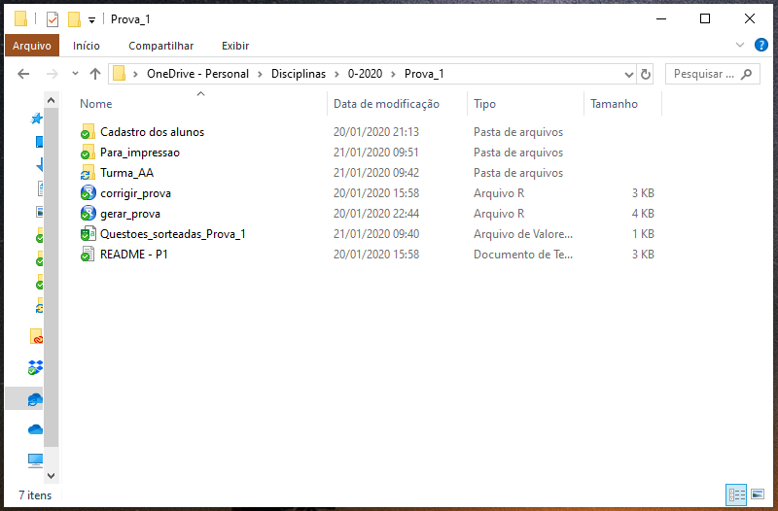
\includegraphics{imagens/pasta_prova1b.png}
\caption{Ilustração da pasta ``Prova\_1''.}
\end{figure}

A pasta de cada turma contém 3 subpastas. Em ``Provas'' estão as provas
individuais de cada aluno separadamente e em ``Solucoes'' estão suas
respectivas resoluções (criadas com base nos arquivos .Rnw da pasta
``Banco\_questoes''). A pasta ``Respostas'' será usada posteriormente na
etapa de correção das provas.

\begin{figure}
\centering
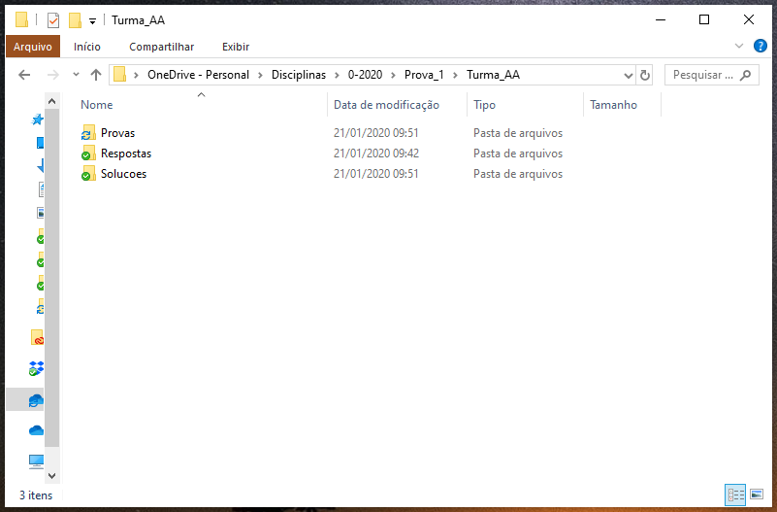
\includegraphics{imagens/pasta_turma.png}
\caption{Ilustração da pasta ``Turma\_AA''.}
\end{figure}

\subsection{Salvando a área de trabalho}

Execute o código a seguir para salvar a área de trabalho das provas
geradas na pasta ``\textbackslash{}PE\textbackslash{}Prova\_1''.

\begin{Shaded}
\begin{Highlighting}[]
\NormalTok{### Salvando a área de trabalho}
\KeywordTok{save.image}\NormalTok{(}\DataTypeTok{file=}\KeywordTok{paste0}\NormalTok{(pasta.provas, }\StringTok{"}\CharTok{\textbackslash{}\textbackslash{}}\StringTok{Area_trabalho_provas_geradas.RData"}\NormalTok{))}
\end{Highlighting}
\end{Shaded}

O processo de geração das provas foi concluído. Na pasta
``Para\_impressao'' estão os arquivos que devem ser enviados para
impressora. Devido ao tamanho dos arquivos, o compartilhamento pode ser
realizado na nuvem, por meio de um link do \(dropbox\), por exemplo.

\subsection{Considerações finais}

Após a impressão dos arquivos, o caderno de questões de cada aluno é
grampeado e a ele anexamos a folha de resposta utilizando um clips para
não ser amassada. Adicionalmente, entregamos ao aluno uma folha com o
formulário, cujo modelo encontra-se em anexo, e uma folha contendo as
tabelas das distribuições Normal e t-student. O formulário e as tabelas
compõem o chamado kit prova, documentos que são impressos apenas uma vez
no semestre e recolhidos e guardados após cada avaliação. Aos alunos
orientamos não escrever nada no kit prova, pois o kit é reaproveitado
inúmeras vezes para reduzir os custos de impressão.

Os alunos são orientados a levarem seu caderno de questões ao terminar a
prova, e guardá-lo para acessar o resultado. No canto superior direito
do caderno de questões de cada aluno há o número de identificação da
prova, que é a senha de acesso do resultado na divulgação das notas.
Considerando que o banco de questões é grande, não há prejuízo os alunos
terem acesso a provas antigas. Além disso, a entrega do caderno de
questões é importante para que os alunos confiram posteriormente a
solução detalhada da sua prova, podendo inclusive reportar erro em
alguma questão do banco.

O código para gerar as provas substitutivas é ligeiramente diferente do
apresentado aqui. No item 3.2.7, adicionamos a variável
``n.provas.turmas'' com um vetor contendo o número de alunos por turma
que irão realizar a prova substitutiva. Os alunos que desejam fazer essa
avaliação respondem a um questionário pelo Moodle demonstrando seu
interesse, e assim também reduzimos os custos de impressão. Além disso,
no item 3.2.5, é possível definir os temas que serão cobrados alterando
a variável ``banco.questoes'', conforme ilustração a seguir:

\begin{Shaded}
\begin{Highlighting}[]
\NormalTok{banco.questoes <-}\StringTok{ }\KeywordTok{list}\NormalTok{(}
  \CommentTok{# Módulo 1}
\NormalTok{  aux[}\KeywordTok{str_detect}\NormalTok{(aux, }\StringTok{"^04_"}\NormalTok{)], }\CommentTok{# Tema 4}
\NormalTok{  aux[}\KeywordTok{str_detect}\NormalTok{(aux, }\StringTok{"^06_"}\NormalTok{)], }\CommentTok{# Tema 6}
\NormalTok{  aux[}\KeywordTok{str_detect}\NormalTok{(aux, }\StringTok{"^08_"}\NormalTok{)], }\CommentTok{# Tema 8}
  \CommentTok{# Módulo 2}
\NormalTok{  aux[}\KeywordTok{str_detect}\NormalTok{(aux, }\StringTok{"^1[1-3]_"}\NormalTok{)], }\CommentTok{# Tema 11, 12 ou 13}
\NormalTok{  aux[}\KeywordTok{str_detect}\NormalTok{(aux, }\StringTok{"^14_"}\NormalTok{)], }\CommentTok{# Tema 14}
\NormalTok{  aux[}\KeywordTok{str_detect}\NormalTok{(aux, }\StringTok{"^18_"}\NormalTok{)], }\CommentTok{# Tema 18}
\NormalTok{  aux[}\KeywordTok{str_detect}\NormalTok{(aux, }\StringTok{"^19|20_"}\NormalTok{)], }\CommentTok{# Tema 19 ou 20 }
  \CommentTok{# Módulo 3}
\NormalTok{  aux[}\KeywordTok{str_detect}\NormalTok{(aux, }\StringTok{"^2[2-4]_"}\NormalTok{)], }\CommentTok{# Tema 22 ou 24}
\NormalTok{  aux[}\KeywordTok{str_detect}\NormalTok{(aux, }\StringTok{"^2[5-7]_"}\NormalTok{)], }\CommentTok{# Tema 25 ou 27}
\NormalTok{  aux[}\KeywordTok{str_detect}\NormalTok{(aux, }\StringTok{"^28|29|30_"}\NormalTok{)] }\CommentTok{# Tema 28, 29 ou 30}
\NormalTok{)}
\end{Highlighting}
\end{Shaded}

\section{Correção das provas}

\subsection{Instruções gerais} \label{subsec:configuracoes}

Além dos pré-requisitos detalhados na Seção \ref{sec:requisitos}, seguem
algumas instruções adicionais para o processo de correção das provas.

As folhas de respostas escaneadas da turma XX devem ser salvas, em
formato pdf, na pasta
``PE\textbackslash{}Prova\_1\textbackslash{}Turma\_XX\textbackslash{}Respostas''.
As configurações utilizadas no escâner interferem fortemente na
qualidade da leitura dos documentos pelo pacote \emph{exams}. Após
diversos testes, a configuração a seguir mostrou-se a mais adequada,
reduzindo o número de erros de leitura e o tamanho dos arquivos gerados.

\begin{itemize}
\tightlist
\item
  Nome do arquivo: Nome da turma (AA, por exemplo).
\item
  Cor: Preto e branco (e não em escala de cinza).
\item
  Resolução: 600 dpi.
\item
  Qualidade: Melhor.
\item
  Opção: Todas as provas em um único arquivo (múltiplas folhas).
\item
  Formato: pdf.
\item
  Orientação: Escanear de cabeça para baixo.
\item
  Claridade: 4 (na escala de 1 a 11).
\item
  Observações: Evitar que as páginas estejam inclinadas.
\end{itemize}

Além disso, o cuidado no preenchimento do cartão de respostas é
primordial para a correta leitura dele. Os aspectos gerais mais
importantes que devem ser reforçados com os alunos são:

\begin{itemize}
\tightlist
\item
  O preenchimento (com caneta azul ou preta) dos campos disponíveis para
  a matrícula e respostas das questões deve ser realizado,
  exclusivamente, por meio da marcação de um ``X'', e não pintando os
  campos citados.
\item
  O cartão de respostas deve ser preservado, de modo que não seja
  amassado, dobrado, manchado ou receba outros tipos de avarias. O aluno
  não deve escrever no verso da folha de respostas.
\item
  Antes de iniciar a prova, o aluno deve conferir se o número de
  identificação da prova (Identidade do documento) é o mesmo na folha de
  respostas e no caderno de questões.
\end{itemize}

A lista completa de instruções impressas nas provas de PE está no modelo
de prova apresentada no apêndice.

Por fim, é recomendável fazer um backup da pasta
``PE\textbackslash{}Prova\_1'' antes de iniciar a correção das provas e
documentar a ocorrência de problemas durante a correção (e o
procedimento executado para correção deles) em um arquivo txt para
registro (``README - P1.txt'').

O código \texttt{corrigir\_prova.R} pode ser executado conforme descrito
a seguir.

\subsection{Carregando os arquivos}

A área de trabalho salva ao final do processo de geração das provas será
carregada no ambiente de trabalho do R, além das funções complementares
ao pacote \emph{exams}.

\begin{Shaded}
\begin{Highlighting}[]
\ControlFlowTok{if}\NormalTok{(}\KeywordTok{length}\NormalTok{(}\KeywordTok{ls}\NormalTok{()) }\OperatorTok{>}\StringTok{ }\DecValTok{0}\NormalTok{) }\KeywordTok{rm}\NormalTok{(}\DataTypeTok{list =} \KeywordTok{ls}\NormalTok{())}
\KeywordTok{setwd}\NormalTok{(}\KeywordTok{choose.dir}\NormalTok{(}\DataTypeTok{default=}\KeywordTok{getwd}\NormalTok{(), }\DataTypeTok{caption=}\StringTok{"Escolha a pasta onde as provas foram salvas"}\NormalTok{))}
\KeywordTok{load}\NormalTok{(}\StringTok{"Area_trabalho_provas_geradas.RData"}\NormalTok{)}
\KeywordTok{source}\NormalTok{(}\KeywordTok{paste0}\NormalTok{(pasta.suplementos, }\StringTok{"}\CharTok{\textbackslash{}\textbackslash{}}\StringTok{Funcoes_Extras.R"}\NormalTok{))  }\CommentTok{# Complementando pacote Exams }
\end{Highlighting}
\end{Shaded}

\subsection{Localizando as pastas}

Esta seção deve ser rodada apenas se as provas tiverem sido geradas em
outro computador. Caso contrário, pular para o próximo passo.

\begin{Shaded}
\begin{Highlighting}[]
\NormalTok{pasta.provas <-}\StringTok{ }\KeywordTok{choose.dir}\NormalTok{(}\DataTypeTok{default=}\KeywordTok{getwd}\NormalTok{(), }
                           \DataTypeTok{caption=}\StringTok{"Escolha a pasta onde as provas foram salvas"}\NormalTok{)}
\NormalTok{pasta.cadastros <-}\StringTok{ }\KeywordTok{choose.dir}\NormalTok{(}\DataTypeTok{default=}\KeywordTok{getwd}\NormalTok{(), }
                              \DataTypeTok{caption=}\StringTok{"Escolha a pasta com os dados dos alunos"}\NormalTok{)}
\NormalTok{pasta.suplementos <-}\StringTok{ }\KeywordTok{choose.dir}\NormalTok{(}\DataTypeTok{default=}\KeywordTok{getwd}\NormalTok{(), }
                            \DataTypeTok{caption=}\StringTok{"Escolha a pasta com os arquivos suplementares"}\NormalTok{)}
\end{Highlighting}
\end{Shaded}

Nesse passo, o programa solicitará que o usuário atualize a localização
de algumas pastas.

\begin{itemize}
\tightlist
\item
  Escolha a pasta onde as provas foram salvas:
  \textbackslash{}PE\textbackslash{}Prova\_1.
\item
  Escolha a pasta com os dados dos alunos:
  \textbackslash{}PE\textbackslash{}Prova\_1\textbackslash{}Cadastro dos
  alunos.
\item
  Escolha a pasta com os arquivos suplementares:
  \textbackslash{}PE\textbackslash{}Suplementos.
\end{itemize}

\subsection{Digitalizando as respostas}

Aqui o cartão de respostas dos alunos será digitalizado. A seguir note
que a função ``digitalizar.respostas()'' contém a opção ``rotate=T''
para indicar que os arquivos foram escaneados de cabeça para baixo (caso
não seja o caso, modificar para ``rotate=F''). Os parâmetros
``threshold'' e ``minrot'' são critérios utilizados internamente na
codificação das informações contidas nas imagens. Para imagens com boa
qualidade (veja Subseção \ref{subsec:configuracoes}), os valores
pré-definidos são satisfatórios, mas caso seja necessário alterá-los,
consulte o \emph{help} da função \emph{nops\_scan}.

\begin{Shaded}
\begin{Highlighting}[]
\NormalTok{### Juntar os metainfos das turmas em um único objeto}
\KeywordTok{juntar.metainfos}\NormalTok{(pasta.provas)}
\NormalTok{metainfo <-}\StringTok{ }\KeywordTok{readRDS}\NormalTok{(}\KeywordTok{paste0}\NormalTok{(pasta.provas, }\StringTok{"}\CharTok{\textbackslash{}\textbackslash{}}\StringTok{Metainfo}\CharTok{\textbackslash{}\textbackslash{}}\StringTok{metainfo.RDS"}\NormalTok{))}

\NormalTok{### Definir as turmas a serem corrigidas}
\NormalTok{corrigir.turmas <-}\StringTok{ }\DecValTok{1}\OperatorTok{:}\NormalTok{n.turmas}

\NormalTok{### Digitalizar as respostas}
\KeywordTok{renomear.arquivos}\NormalTok{(pasta.provas, corrigir.turmas)}
\KeywordTok{gerar.cadastros}\NormalTok{(pasta.provas, corrigir.turmas)}
\KeywordTok{digitalizar.respostas}\NormalTok{(pasta.provas, corrigir.turmas, }\DataTypeTok{rotate=}\NormalTok{T, }
                      \DataTypeTok{threshold=}\KeywordTok{c}\NormalTok{(}\FloatTok{0.04}\NormalTok{, }\FloatTok{0.6}\NormalTok{),  }\DataTypeTok{minrot=}\FloatTok{0.001}\NormalTok{)}
\end{Highlighting}
\end{Shaded}

Nesta etapa será criado um arquivo chamado ``metainfo.Rds'' na pasta
``Metainfo''. Este arquivo contém os metadados produzidos, sendo usado
internamente durante o processo de correção das provas.

Além disso, na pasta de cada turma
``\textbackslash{}Turma\_XX\textbackslash{}Respostas'', os arquivos
``Cadastro.csv'' e ``nops\_scan\_x.zip'' serão criados. O primeiro
contém os dados do aluno (nome, matrícula) e o número de identificação
da sua prova. O segundo contém todas as imagens (cartão de resposta)
lidas pelo programa e um arquivo ``Daten.txt'' com as informações
extraídas dessas imagens.

Neste momento é necessário abrir o arquivo ``Daten.txt'' e verificar se
há alguma linha com a palavra ``ERROR'', indicando erro de leitura em
alguma prova. Caso haja alguns erros, recomenda-se escanear as provas
novamente. Alternativamente, os dados das provas não lidas poderão ser
inseridos manualmente. Para tanto, abra a imagem correspondente no
arquivo zipado ``nops\_scan\_x.zip'' e insira os dados na linha que
apresentou erro. Para facilitar, no lugar do ``ERROR'', copie e cole a
linha anterior (como modelo) e altere todos os dados necessários. Note
que a codificação da marcação do aluno segue a seguinte lógica: a
(10000), b (01000), c (00100), d (00010), e (00001). Após as alterações,
salve o arquivo ``Daten.txt'' e, ao fechar a janela do arquivo zipado
``nops\_scan\_x.zip'', selecione a opção de aceitar mudanças no arquivo
zip na caixa de diálogo que aparecerá.

Caso algum aluno tenha errado a marcação da folha de respostas
(preenchendo todo o quadrado, por exemplo), o arquivo ``Daten.txt''
também pode ser alterado nesse momento para inserir manualmente as
informações.

\subsection{Checando as leituras}

Execute o código a seguir para checar as leituras dos cartões.

\begin{Shaded}
\begin{Highlighting}[]
\NormalTok{### Checar leituras em respostas onde mais de um item foi marcado}
\KeywordTok{checar.leituras}\NormalTok{(pasta.provas, corrigir.turmas)}
\NormalTok{leitura.duvidosa <-}\StringTok{ }\NormalTok{leitura.correta <-}\StringTok{ }\KeywordTok{procurar.erros}\NormalTok{(pasta.provas, corrigir.turmas)}
\KeywordTok{fix}\NormalTok{(leitura.correta)}
\KeywordTok{write.table}\NormalTok{(leitura.correta, }\KeywordTok{paste0}\NormalTok{(pasta.provas, }\StringTok{"}\CharTok{\textbackslash{}\textbackslash{}}\StringTok{leitura.correta.txt"}\NormalTok{))}
\KeywordTok{corrigir.leitura}\NormalTok{(leitura.correta, pasta.provas, corrigir.turmas)}
\KeywordTok{corrigir.provas}\NormalTok{(corrigir.turmas)}
\end{Highlighting}
\end{Shaded}

Primeiramente, as leituras serão checadas para verificar se as
matrículas que os alunos preencheram estão de acordo com as matrículas
registradas no cadastro dos alunos. Aqui é normal aparecer algumas
discordâncias, seja porque o aluno marcou errado (mais provável), ou
deixou em branco, ou o sistema não leu corretamente (pode acontecer). Em
todos esses casos, para corrigir a matrícula, deve-se digitar
manualmente o número correto. Para isso, digite o número de matrícula
que o aluno escreveu na prova com base na imagem apresentada ao lado. Em
geral, a marcação com ``x'' está errada, mas o número informado está
correto. Caso este número também tenha sido escrito errado (raro, mas
acontece), o sistema vai continuar acusando erro nessa prova, e o número
de matrícula correto do aluno pode ser encontrado no cadastro com base
no seu nome completo.

Essa etapa de correção das matrículas é a mais dispendiosa, por isso
vale reforçar a atenção dos alunos com esse ponto para reduzir os erros.

Em seguida, as leituras serão checadas para verificar se alguma questão
tem dupla marcação. Se houver, o programa vai abrir uma janela com os
dados da respectiva prova para alteração manual. Lembrando que a
codificação segue a seguinte lógica: a (10000), b (01000), c (00100), d
(00010), e (00001). Recomenda-se abrir a imagem da prova correspondente
(busque o arquivo em ``nops\_scan\_x.zip'' na pasta
``Prova\_1\textbackslash{}Turma\_XX\textbackslash{}Respostas'') para
averiguar o motivo da dupla marcação (falha do aluno ou do sistema).

Após essas correções manuais, as provas serão corrigidas e alguns
gráficos gerais serão apresentados no R.

\subsection{Gerando os resultados}

Além das notas, cada aluno recebe um arquivo contendo a sua folha de
respostas, o gabarito correto e a solução detalhada da sua prova. Este
arquivo é codificado com uma senha, esta é o número de identificação da
prova, que também está impressa no canto superior direito do caderno de
questões de cada aluno. Lembrando que os alunos levam seu caderno de
questões ao terminar a prova, e devem guardá-lo para acessar o resultado
com essa senha.

\begin{Shaded}
\begin{Highlighting}[]
\NormalTok{### Gerar os resultados}
\NormalTok{diretorio.resultados <-}\StringTok{ }\KeywordTok{paste0}\NormalTok{(pasta.provas, }\StringTok{"}\CharTok{\textbackslash{}\textbackslash{}}\StringTok{Resultados"}\NormalTok{) }
\KeywordTok{criar.resumos}\NormalTok{(pasta.provas, diretorio.resultados, corrigir.turmas)}
\KeywordTok{gerar.espelhos}\NormalTok{(pasta.provas, diretorio.resultados, corrigir.turmas)}
\KeywordTok{converter.html2pdf}\NormalTok{(corrigir.turmas)  }\CommentTok{# Converter os espelhos de prova para pdf }
\NormalTok{banco.respostas <-}\StringTok{ }\KeywordTok{gerar.banco.dados}\NormalTok{(corrigir.turmas)  }\CommentTok{# Banco das respostas dos alunos}
\KeywordTok{juntar.arquivos.divulgacao}\NormalTok{(corrigir.turmas)  }\CommentTok{# Juntar os arquivos para divulgação}
\KeywordTok{inserir.senha.pdf}\NormalTok{(corrigir.turmas)}
\end{Highlighting}
\end{Shaded}

Nessa seção, o sistema faz a organização desses arquivos para
apresentação do resultado da prova aos alunos. Uma pasta chamada
``Resultados'' é criada em ``\textbackslash{}Prova\_1\textbackslash{}''
contendo uma planilha por turma com as notas. Além disso, na pasta
``Prova\_1\textbackslash{}Resultados\textbackslash{}Turma\_XX'', estão
os arquivos de cada aluno, cujo nome é o número da matrícula e a senha é
o número de identificação da prova. Esses arquivos pdf são
disponibilizados no Moodle.

Considerando a estrutura da disciplina de Probabilidade e Estatística,
com 3 provas e uma prova substitutiva, as menções provisórias podem ser
geradas após a prova 3 rodando a linha a seguir.

\begin{Shaded}
\begin{Highlighting}[]
\NormalTok{### Gerar menções provisórias}
\KeywordTok{gerar.mencoes.provisorias}\NormalTok{(corrigir.turmas)}
\end{Highlighting}
\end{Shaded}

A função ``gerar.mencoes.provisorias()'' reuni o resultado das 3 provas
em uma única planilha e calcula a menção provisória (anterior à prova
substitutiva) da disciplina de Probabilidade e Estatística considerando
os pesos estabelecidos. Portanto, essa função deve ser usada apenas após
a correção da Prova 3. Observação: caso professores façam ajustes da
nota em seus arquivos pessoais, as alterações serão perdidas no momento
da junção das planilhas.

De forma análoga, durante a correção das provas substitutivas, a menção
final pode ser gerada rodando a linha a seguir.

\begin{Shaded}
\begin{Highlighting}[]
\KeywordTok{gerar.mencoes.finais}\NormalTok{(}\DecValTok{1}\OperatorTok{:}\NormalTok{n.turmas, diretorio.resultados)}
\end{Highlighting}
\end{Shaded}

A função ``gerar.mencoes.finais()'' reuni o resultado das 4 provas em
uma única planilha e calcula a nota final considerando a substituição da
menor nota pela nota da prova substitutiva (se beneficiar o aluno).
Observação: caso professores façam ajustes da nota em seus arquivos
pessoais, as alterações serão perdidas no momento da junção das
planilhas.

\subsection{Salvando a área de trabalho}

Execute o código a seguir para salvar a área de trabalho das provas
corrigidas na pasta ``\textbackslash{}PE\textbackslash{}Prova\_1''.

\begin{Shaded}
\begin{Highlighting}[]
\NormalTok{### Salvando a área de trabalho}
\KeywordTok{save.image}\NormalTok{(}\DataTypeTok{file=}\KeywordTok{paste0}\NormalTok{(pasta.provas, }\StringTok{"}\CharTok{\textbackslash{}\textbackslash{}}\StringTok{Area_trabalho_provas_corrigidas.RData"}\NormalTok{))}
\end{Highlighting}
\end{Shaded}

Pronto! Agora é só disponibilizar os arquivos pdf codificados com senha
aos alunos.

\subsection{Considerações finais}

Caso tenha ocorrido algum problema em uma questão após a aplicação das
provas, é possível realizar algumas intervenções para ajuste na nota do
aluno.

\begin{itemize}
\tightlist
\item
  Caso 1: A resposta correta está em outra alternativa
\end{itemize}

Nesse caso, é possível alterar o código .Rnw da questão com problema
para indicar que a resposta correta está em outra alternativa. Na pasta
``\textbackslash{}PE\textbackslash{}Banco\_questoes'', abra o arquivo da
questão correspondente e identifique em qual posição do vetor ``alt''
encontra-se a alternativa correta (ver seção do código ``\#\# gerando
alternativas''). Troque a linha ``solutions \textless{}- c(TRUE,
rep(FALSE, 4))'' por ``solutions \textless{}- c(F, T, F, F, F)'', se a
segunda alternativa estiver correta, e assim por diante. Esta é a única
linha que precisa ser alterada. Em seguida, execute novamente o código
``gerar\_prova.R'' sem realizar nenhuma alteração nele (mantenha
inclusive a mesma semente). Dessa forma, o arquivo metainfo será
atualizado e, ao corrigir novamente as provas, a alternativa correta
será devidamente identificada. Portanto, execute o código
``corrigir\_prova.R'' novamente também sem nenhuma modificação. Dessa
forma, tanto as notas dos alunos quanto os resultados que são enviados a
eles (ver anexo 2: Resultados do exame) serão atualizados com o novo
gabarito da questão.

Observação: Em todos os códigos .Rnw, a solução correta é armazenada na
primeira posição do vetor ``alt'' (ou seja, ``alt{[}1{]} \textless{}-
solução correta''), e posteriormente essa posição é aleatorizada.
Portanto, recomenda-se que faça a alteração detalhada no parágrafo
anterior para corrigir o problema dessa avaliação que já foi realizada,
mas depois modifique o código para o padrão das demais questões, ou
seja, ``alt{[}1{]} \textless{}- solução correta'' e ``solutions
\textless{}- c(TRUE, rep(FALSE, 4))''.

\begin{itemize}
\tightlist
\item
  Caso 2: A questão não apresenta nenhuma alternativa correta
\end{itemize}

Nesse caso a questão precisa ser anulada, e o ponto pode ser dado
diretamente ao aluno ou redistribuído para as demais questões da prova.
Em ambos os casos, as notas podem ser diretamente alteradas nas
planilhas excel da pasta
``PE\textbackslash{}Prova\_x\textbackslash{}Resultados''. Entretanto, os
arquivos enviados aos alunos (ver anexo 2: Resultados do exame) não
serão atualizados. Os alunos podem ser apenas notificados que receberão
um ponto a mais caso tenham errado a questão (se o ponto for dado a
todos, por exemplo).

Para redistribuir os pontos entre as demais questões, é possível rodar
as provas novamente para atualizar tanto as notas quanto os arquivos
enviados aos alunos (ver anexo 2: Resultados do exame). Nesse caso,
modifique as linhas a seguir do código ``gerar\_prova.R'' (ver seção
3.2.5) para anular a primeira questão da prova, por exemplo, e
redistribuir os pontos.

Substituindo

\begin{Shaded}
\begin{Highlighting}[]
\CommentTok{# Definindo o valor de cada questão}
\NormalTok{pontos <-}\StringTok{ }\KeywordTok{round}\NormalTok{(total.pontos}\OperatorTok{*}\KeywordTok{rep}\NormalTok{(}\DecValTok{1}\OperatorTok{/}\NormalTok{n.questoes, n.questoes), }\DecValTok{2}\NormalTok{)  }
\NormalTok{pontos[}\DecValTok{1}\NormalTok{] <-}\StringTok{ }\KeywordTok{round}\NormalTok{(total.pontos}\OperatorTok{-}\KeywordTok{sum}\NormalTok{(pontos[}\OperatorTok{-}\DecValTok{1}\NormalTok{]), }\DecValTok{2}\NormalTok{)}
\end{Highlighting}
\end{Shaded}

por

\begin{Shaded}
\begin{Highlighting}[]
\CommentTok{# Definindo o valor de cada questão}
\NormalTok{pontos <-}\StringTok{ }\KeywordTok{c}\NormalTok{(}\DecValTok{0}\NormalTok{,}\KeywordTok{round}\NormalTok{(total.pontos}\OperatorTok{*}\KeywordTok{rep}\NormalTok{(}\DecValTok{1}\OperatorTok{/}\NormalTok{(n.questoes}\OperatorTok{-}\DecValTok{1}\NormalTok{), n.questoes}\OperatorTok{-}\DecValTok{1}\NormalTok{), }\DecValTok{2}\NormalTok{))  }
\NormalTok{pontos[}\DecValTok{1}\NormalTok{] <-}\StringTok{ }\KeywordTok{round}\NormalTok{(total.pontos}\OperatorTok{-}\KeywordTok{sum}\NormalTok{(pontos[}\OperatorTok{-}\DecValTok{1}\NormalTok{]), }\DecValTok{2}\NormalTok{)}
\end{Highlighting}
\end{Shaded}

Recomenda-se registrar as intervenções necessárias durante o processo de
correção das provas no arquivo ``README - P1.txt'' para manter controle
do processo.

\newpage

\BgThispage
\appendix
\chapter{Apêndice}

\newpage

\fakesection{Exemplo de Prova}
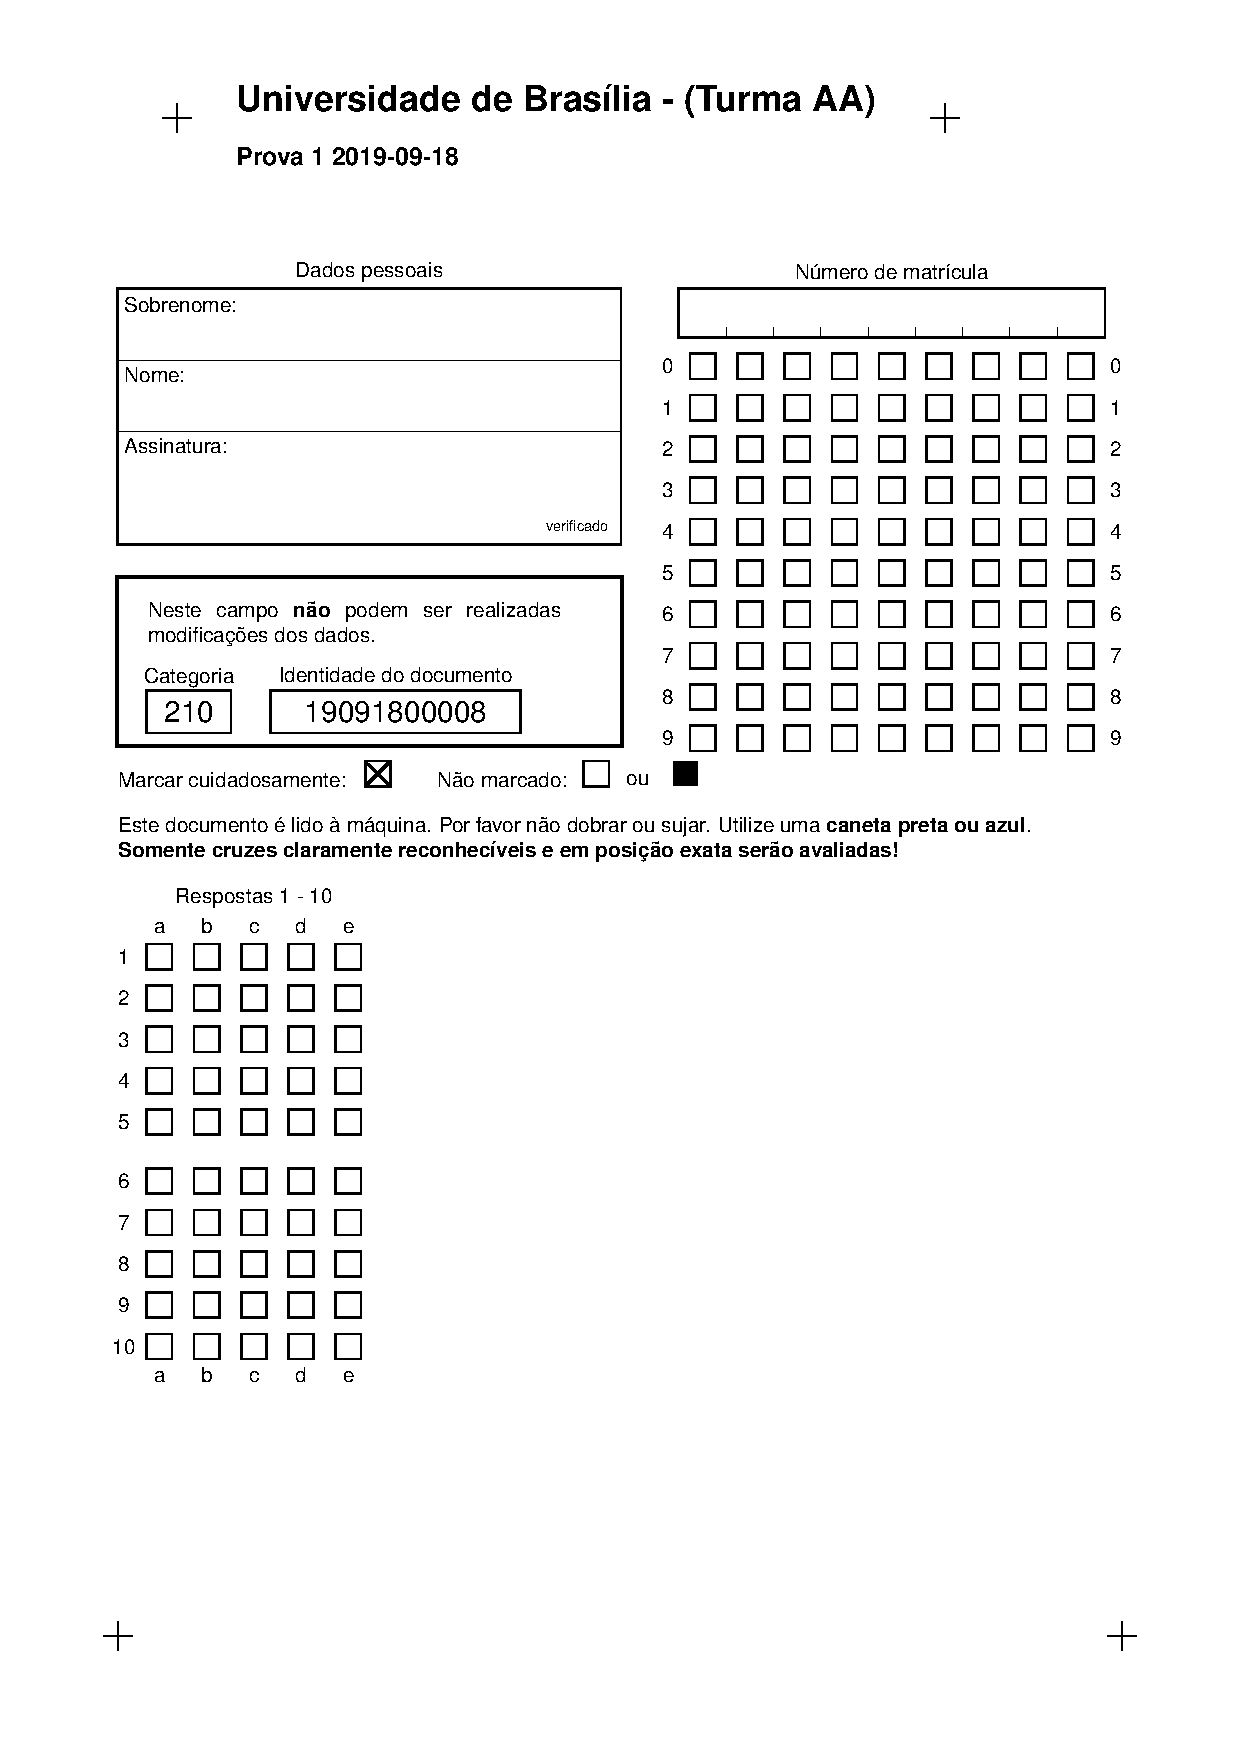
\includepdf[fitpaper=TRUE, pages={1-5}]{imagens/Prova_1_AA_08.pdf}

\newpage

\fakesection{Exemplo de Resultado}
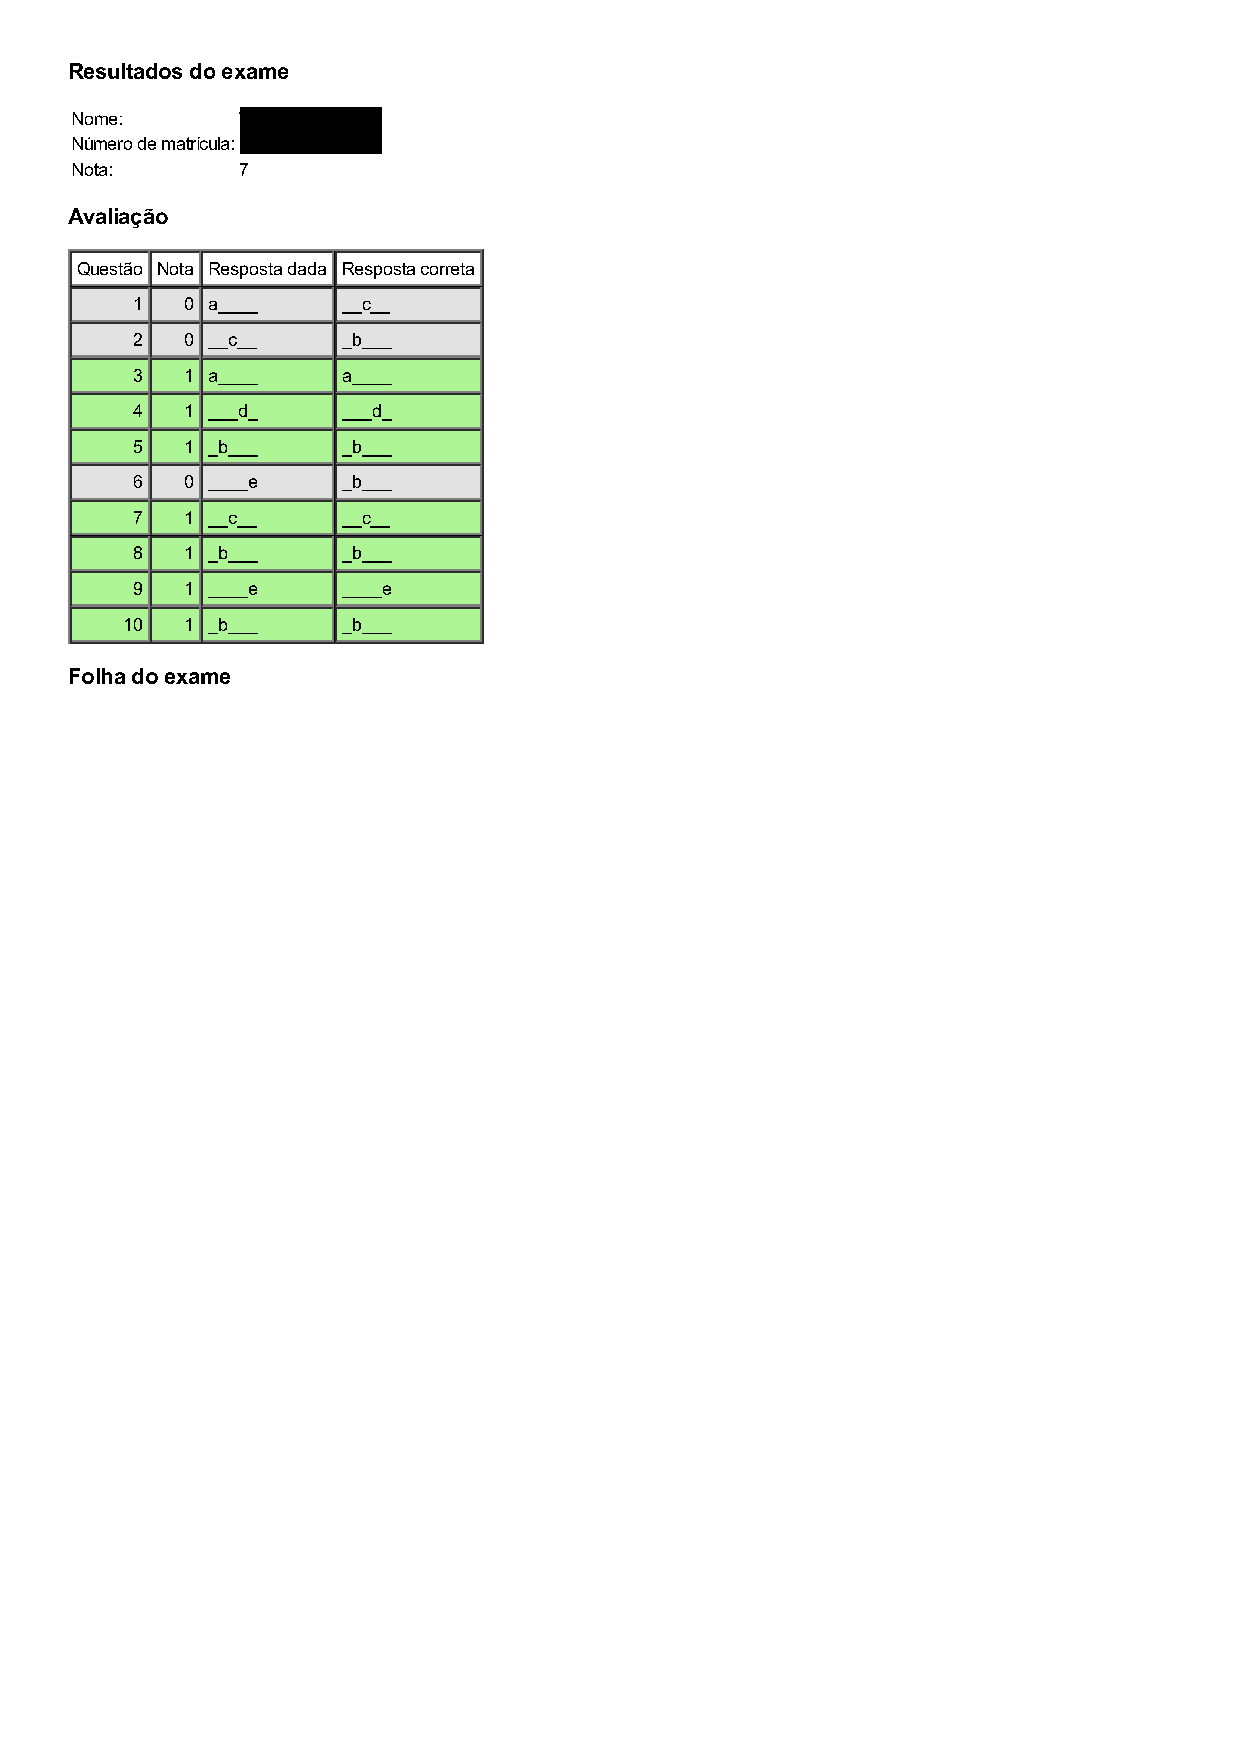
\includepdf[fitpaper=TRUE, pages={1-8}]{imagens/170170586-desbloqueado-editado.pdf}

\newpage

\fakesection{Lista de Fórmulas}
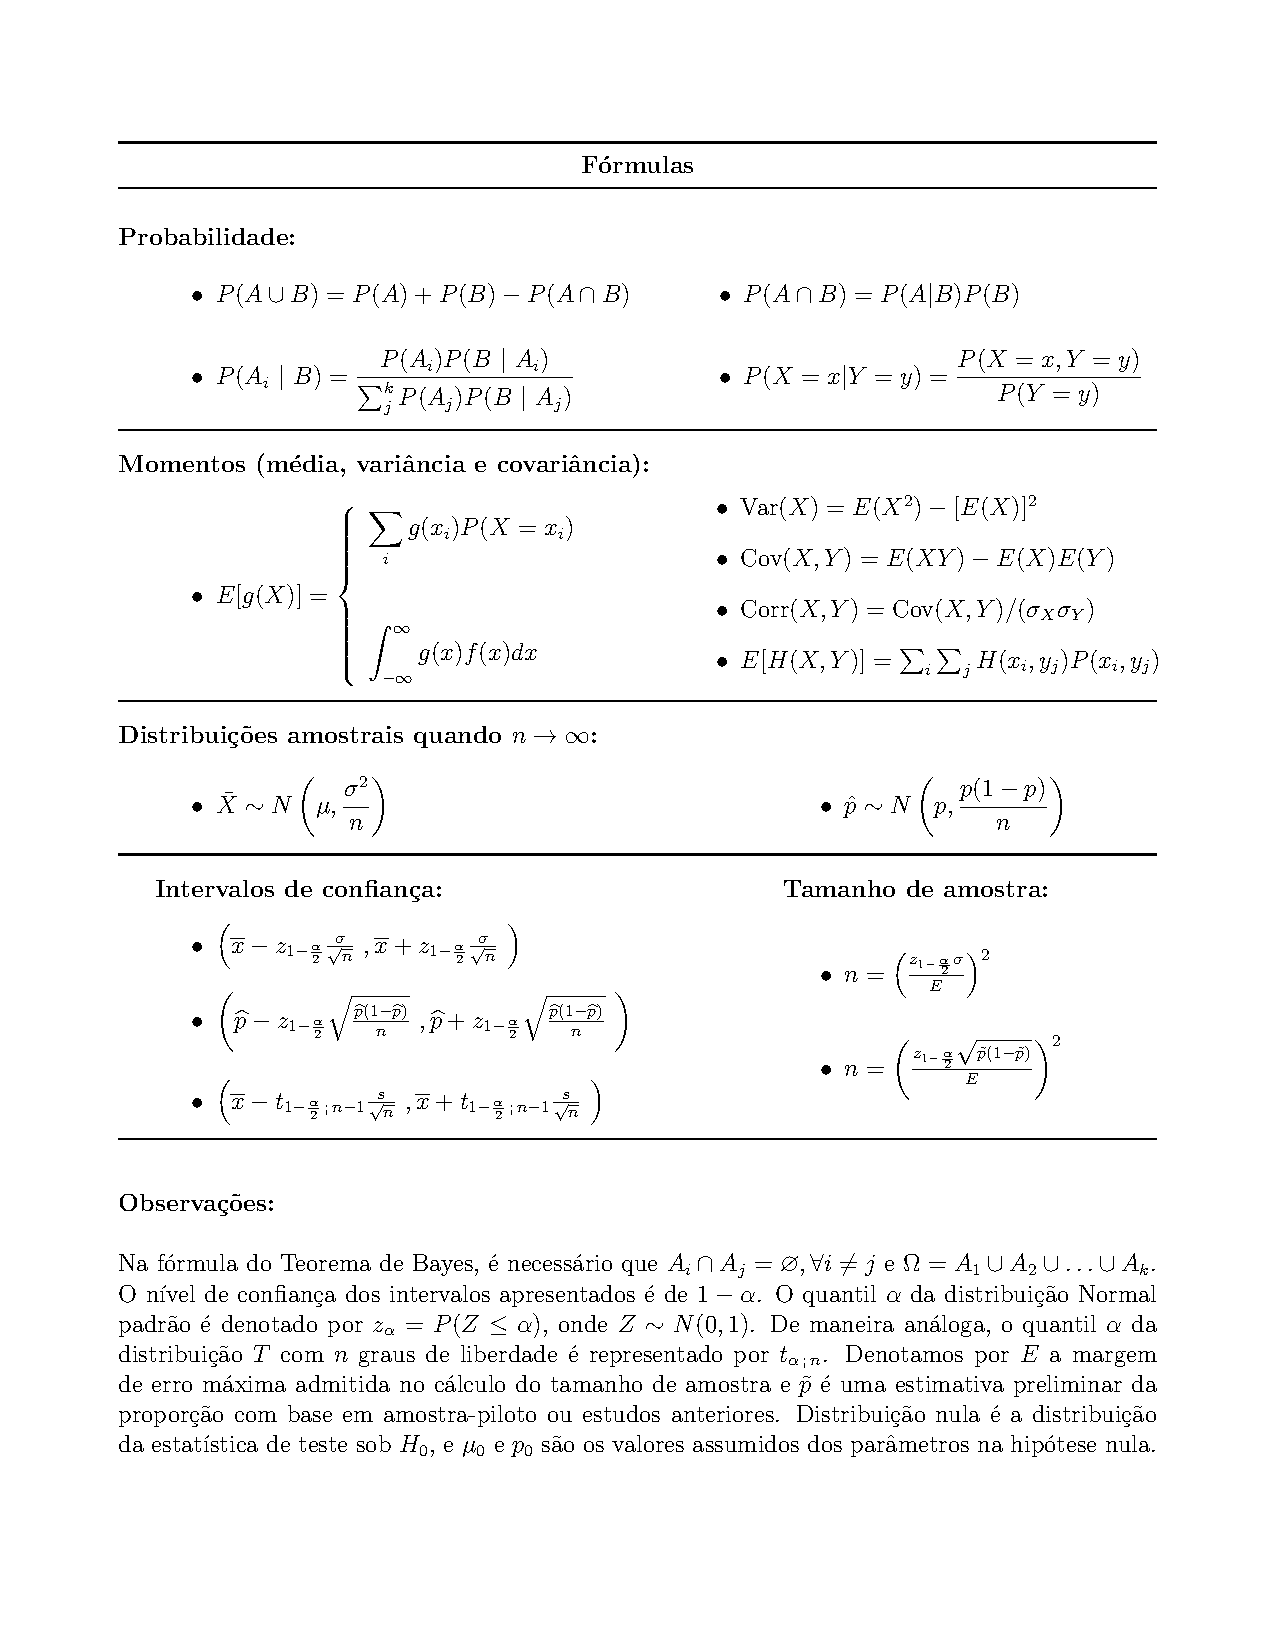
\includepdf[fitpaper=TRUE, pages={1-2}]{imagens/Formulario.pdf}

\newpage

\fakesection{Tabelas dos parâmetros das questões} \label{sec:tabelas}

\begin{longtable}{l|c|c|c|c|c|c|c|c|c}
\caption{\label{tab:unnamed-chunk-31}Parâmetros para cada questão da Prova 1 . n=número de respondentes; p1, p2 e p3: probabilidade deacerto de um aluno com habilidade -3 (mínima), 0 (mediana) e 3 (maxima).}\\
\hline
Tema & Q & a & b & c & n & \% acerto & p1 & p2 & p3\\
\hline
\endfirsthead
\caption[]{Parâmetros para cada questão da Prova 1 . n=número de respondentes; p1, p2 e p3: probabilidade deacerto de um aluno com habilidade -3 (mínima), 0 (mediana) e 3 (maxima).  (continuação)}\\
\hline
Tema & Q & a & b & c & n & \% acerto & p1 & p2 & p3\\
\hline
\endhead
medida\_probabilidade & 01 & 0.6 & 1.6 & 0.17 & 44 & 27 & 20 & 32 & 60\\
\hline
medida\_probabilidade & 02 & 1.1 & 0.7 & 0.21 & 86 & 50 & 22 & 49 & 95\\
\hline
medida\_probabilidade & 05 & 1.0 & 1.5 & 0.15 & 52 & 31 & 16 & 32 & 86\\
\hline
medida\_probabilidade & 06 & 1.1 & -0.5 & 0.24 & 48 & 71 & 28 & 71 & 98\\
\hline
medida\_probabilidade & 07 & 1.0 & 0.8 & 0.20 & 39 & 46 & 22 & 46 & 92\\
\hline
medida\_probabilidade & 09 & 0.6 & -0.3 & 0.25 & 95 & 67 & 39 & 67 & 90\\
\hline
medida\_probabilidade & 10 & 0.9 & -0.1 & 0.24 & 64 & 66 & 30 & 65 & 96\\
\hline
propriedade\_probabilidade & 01 & 1.1 & 0.7 & 0.20 & 45 & 49 & 21 & 48 & 95\\
\hline
propriedade\_probabilidade & 04 & 1.6 & -1.3 & 0.24 & 98 & 79 & 27 & 84 & 100\\
\hline
propriedade\_probabilidade & 05 & 0.7 & 1.3 & 0.18 & 90 & 37 & 21 & 37 & 74\\
\hline
propriedade\_probabilidade & 07 & 0.7 & 0.5 & 0.22 & 56 & 52 & 28 & 52 & 86\\
\hline
propriedade\_probabilidade & 08 & 1.6 & 0.3 & 0.20 & 48 & 54 & 21 & 55 & 99\\
\hline
propriedade\_probabilidade & 09 & 0.9 & -0.7 & 0.26 & 52 & 77 & 35 & 75 & 98\\
\hline
propriedade\_probabilidade & 10 & 0.7 & -1.2 & 0.25 & 39 & 85 & 46 & 82 & 97\\
\hline
probabilidade\_total & 01 & 1.2 & -1.3 & 0.24 & 55 & 84 & 31 & 84 & 100\\
\hline
probabilidade\_total & 03 & 0.8 & -1.7 & 0.25 & 132 & 87 & 48 & 88 & 99\\
\hline
probabilidade\_total & 04 & 1.5 & -0.7 & 0.23 & 98 & 72 & 25 & 74 & 100\\
\hline
probabilidade\_total & 05 & 1.3 & -1.1 & 0.24 & 45 & 80 & 28 & 81 & 100\\
\hline
probabilidade\_total & 07 & 1.4 & -1.1 & 0.24 & 50 & 76 & 28 & 80 & 100\\
\hline
probabilidade\_total & 08 & 1.3 & -0.8 & 0.24 & 48 & 75 & 27 & 76 & 99\\
\hline
teorema\_Bayes & 02 & 0.8 & -0.1 & 0.25 & 100 & 66 & 32 & 65 & 95\\
\hline
teorema\_Bayes & 03 & 0.7 & 1.3 & 0.20 & 89 & 38 & 23 & 39 & 75\\
\hline
teorema\_Bayes & 05 & 0.7 & 1.2 & 0.19 & 45 & 38 & 21 & 39 & 79\\
\hline
teorema\_Bayes & 06 & 1.7 & -0.7 & 0.23 & 52 & 73 & 24 & 74 & 100\\
\hline
teorema\_Bayes & 07 & 1.2 & 0.1 & 0.22 & 48 & 60 & 24 & 60 & 98\\
\hline
teorema\_Bayes & 10 & 1.4 & -0.3 & 0.20 & 94 & 64 & 21 & 66 & 99\\
\hline
variaveis\_aleatorias & 01 & 1.2 & 0.7 & 0.19 & 46 & 48 & 20 & 47 & 96\\
\hline
variaveis\_aleatorias & 03 & 0.9 & -0.5 & 0.25 & 83 & 72 & 33 & 71 & 97\\
\hline
variaveis\_aleatorias & 04 & 1.6 & 0.2 & 0.21 & 93 & 58 & 21 & 58 & 99\\
\hline
variaveis\_aleatorias & 05 & 0.5 & -2.7 & 0.27 & 52 & 100 & 84 & 95 & 99\\
\hline
variaveis\_aleatorias & 06 & 1.0 & 0.0 & 0.23 & 48 & 62 & 26 & 62 & 96\\
\hline
variaveis\_aleatorias & 07 & 1.1 & -1.5 & 0.25 & 50 & 84 & 35 & 86 & 99\\
\hline
variaveis\_aleatorias & 09 & 0.9 & 0.6 & 0.22 & 40 & 50 & 25 & 51 & 92\\
\hline
variaveis\_aleatorias & 10 & 1.1 & -1.2 & 0.24 & 16 & 88 & 32 & 81 & 99\\
\hline
distribuicao\_binomial & 01 & 1.7 & -0.1 & 0.21 & 88 & 60 & 21 & 63 & 100\\
\hline
distribuicao\_binomial & 02 & 0.9 & -0.1 & 0.23 & 45 & 64 & 29 & 63 & 95\\
\hline
distribuicao\_binomial & 04 & 1.1 & -0.2 & 0.23 & 100 & 66 & 27 & 66 & 98\\
\hline
distribuicao\_binomial & 06 & 1.9 & 0.7 & 0.15 & 96 & 46 & 16 & 44 & 100\\
\hline
distribuicao\_binomial & 07 & 0.8 & 1.0 & 0.20 & 16 & 38 & 22 & 44 & 85\\
\hline
distribuicao\_binomial & 10 & 1.0 & -0.7 & 0.25 & 44 & 77 & 32 & 75 & 98\\
\hline
distribuicao\_geometrica & 01 & 0.5 & -1.6 & 0.26 & 48 & 90 & 63 & 87 & 97\\
\hline
distribuicao\_geometrica & 04 & 1.2 & 0.2 & 0.22 & 64 & 58 & 23 & 57 & 97\\
\hline
distribuicao\_geometrica & 05 & 1.5 & 0.5 & 0.18 & 97 & 53 & 19 & 50 & 98\\
\hline
distribuicao\_geometrica & 06 & 1.1 & 0.0 & 0.22 & 135 & 61 & 25 & 61 & 97\\
\hline
distribuicao\_geometrica & 10 & 0.7 & -0.7 & 0.24 & 44 & 77 & 40 & 75 & 95\\
\hline
distribuicao\_hipergeometrica & 01 & 1.7 & -1.2 & 0.23 & 62 & 77 & 24 & 81 & 100\\
\hline
distribuicao\_hipergeometrica & 02 & 0.7 & 0.9 & 0.22 & 50 & 44 & 25 & 46 & 84\\
\hline
distribuicao\_hipergeometrica & 03 & 1.4 & -0.5 & 0.22 & 92 & 70 & 24 & 70 & 99\\
\hline
distribuicao\_hipergeometrica & 05 & 1.4 & 0.0 & 0.22 & 48 & 60 & 23 & 62 & 99\\
\hline
distribuicao\_hipergeometrica & 08 & 1.4 & 0.9 & 0.18 & 52 & 44 & 18 & 42 & 97\\
\hline
distribuicao\_hipergeometrica & 09 & 0.9 & 0.1 & 0.24 & 40 & 60 & 29 & 61 & 94\\
\hline
distribuicao\_hipergeometrica & 10 & 0.8 & -1.0 & 0.25 & 84 & 80 & 40 & 80 & 98\\
\hline
distribuicao\_poisson & 01 & 1.2 & 1.1 & 0.16 & 40 & 35 & 17 & 39 & 94\\
\hline
distribuicao\_poisson & 03 & 1.0 & 1.0 & 0.17 & 89 & 43 & 19 & 41 & 91\\
\hline
distribuicao\_poisson & 04 & 0.5 & -1.1 & 0.25 & 48 & 83 & 53 & 81 & 96\\
\hline
distribuicao\_poisson & 05 & 1.2 & 0.0 & 0.22 & 91 & 63 & 24 & 62 & 98\\
\hline
distribuicao\_poisson & 06 & 1.0 & 0.3 & 0.22 & 94 & 57 & 25 & 57 & 96\\
\hline
distribuicao\_poisson & 07 & 1.7 & 1.1 & 0.15 & 50 & 34 & 15 & 37 & 98\\
\hline
distribuicao\_poisson & 08 & 0.4 & 1.4 & 0.19 & 16 & 25 & 24 & 36 & 55\\
\hline
aproximacao\_poisson\_binomial & 02 & 1.6 & -0.9 & 0.22 & 181 & 74 & 24 & 77 & 100\\
\hline
aproximacao\_poisson\_binomial & 04 & 1.3 & -0.2 & 0.23 & 96 & 65 & 25 & 66 & 99\\
\hline
aproximacao\_poisson\_binomial & 05 & 1.3 & -0.5 & 0.23 & 48 & 69 & 26 & 71 & 99\\
\hline
aproximacao\_poisson\_binomial & 06 & 1.3 & 0.0 & 0.22 & 16 & 62 & 23 & 62 & 98\\
\hline
aproximacao\_poisson\_binomial & 07 & 0.9 & 1.2 & 0.17 & 48 & 35 & 18 & 37 & 85\\
\hline
aproximacao\_poisson\_binomial & 08 & 0.8 & 1.3 & 0.18 & 39 & 33 & 20 & 36 & 80\\
\hline
\end{longtable}

\begin{longtable}{l|c|c|c|c|c|c|c|c|c}
\caption{\label{tab:unnamed-chunk-31}Parâmetros para cada questão da Prova 2 . n=número de respondentes; p1, p2 e p3: probabilidade deacerto de um aluno com habilidade -3 (mínima), 0 (mediana) e 3 (maxima).}\\
\hline
Tema & Q & a & b & c & n & \% acerto & p1 & p2 & p3\\
\hline
\endfirsthead
\caption[]{Parâmetros para cada questão da Prova 2 . n=número de respondentes; p1, p2 e p3: probabilidade deacerto de um aluno com habilidade -3 (mínima), 0 (mediana) e 3 (maxima).  (continuação)}\\
\hline
Tema & Q & a & b & c & n & \% acerto & p1 & p2 & p3\\
\hline
\endhead
funcao\_densidade & 01 & 1.2 & 1.5 & 0.15 & 103 & 32 & 16 & 32 & 92\\
\hline
funcao\_densidade & 03 & 1.2 & 0.0 & 0.22 & 49 & 61 & 24 & 62 & 98\\
\hline
funcao\_densidade & 04 & 1.0 & 0.3 & 0.22 & 134 & 58 & 26 & 57 & 95\\
\hline
funcao\_densidade & 05 & 0.7 & -0.6 & 0.24 & 49 & 71 & 37 & 73 & 95\\
\hline
funcao\_densidade & 06 & 1.3 & -0.4 & 0.24 & 52 & 67 & 26 & 69 & 99\\
\hline
funcao\_densidade & 08 & 1.1 & -1.1 & 0.25 & 44 & 80 & 33 & 81 & 99\\
\hline
distribuicao\_acumulada & 01 & 1.5 & 0.1 & 0.21 & 52 & 58 & 22 & 59 & 99\\
\hline
distribuicao\_acumulada & 07 & 0.8 & -0.5 & 0.25 & 104 & 70 & 34 & 71 & 96\\
\hline
distribuicao\_acumulada & 08 & 1.0 & 0.5 & 0.21 & 49 & 49 & 24 & 52 & 93\\
\hline
distribuicao\_acumulada & 09 & 0.7 & -0.5 & 0.25 & 47 & 74 & 38 & 72 & 95\\
\hline
distribuicao\_acumulada & 10 & 1.1 & 0.0 & 0.24 & 90 & 62 & 27 & 63 & 97\\
\hline
momentos & 01 & 0.9 & -0.3 & 0.24 & 49 & 65 & 30 & 68 & 97\\
\hline
momentos & 04 & 0.6 & 1.5 & 0.18 & 44 & 30 & 20 & 34 & 67\\
\hline
momentos & 06 & 1.3 & -0.3 & 0.22 & 52 & 65 & 25 & 68 & 99\\
\hline
momentos & 07 & 0.7 & -0.8 & 0.25 & 16 & 81 & 43 & 76 & 96\\
\hline
momentos & 08 & 0.6 & 1.5 & 0.19 & 96 & 34 & 21 & 34 & 67\\
\hline
momentos & 10 & 1.5 & 0.8 & 0.16 & 42 & 43 & 16 & 43 & 98\\
\hline
distribuicao\_exponencial & 03 & 0.9 & 0.9 & 0.19 & 185 & 44 & 21 & 43 & 88\\
\hline
distribuicao\_exponencial & 05 & 1.4 & 1.0 & 0.17 & 52 & 40 & 18 & 41 & 97\\
\hline
distribuicao\_exponencial & 06 & 0.8 & 1.1 & 0.19 & 16 & 31 & 22 & 42 & 82\\
\hline
distribuicao\_exponencial & 07 & 0.7 & 0.9 & 0.21 & 97 & 43 & 25 & 45 & 80\\
\hline
distribuicao\_exponencial & 08 & 0.8 & 0.5 & 0.22 & 81 & 52 & 26 & 51 & 89\\
\hline
distribuicao\_normal & 01 & 1.3 & 1.2 & 0.17 & 49 & 37 & 17 & 37 & 95\\
\hline
distribuicao\_normal & 02 & 1.7 & 0.4 & 0.18 & 91 & 53 & 18 & 51 & 99\\
\hline
distribuicao\_normal & 05 & 0.8 & 1.5 & 0.18 & 133 & 34 & 19 & 33 & 76\\
\hline
distribuicao\_normal & 06 & 0.9 & 1.5 & 0.18 & 94 & 33 & 19 & 34 & 79\\
\hline
distribuicao\_normal & 07 & 1.1 & 0.3 & 0.22 & 48 & 54 & 24 & 57 & 96\\
\hline
distribuicao\_normal & 09 & 1.0 & -0.4 & 0.24 & 16 & 69 & 30 & 69 & 97\\
\hline
aproximacao\_normal\_binomial & 01 & 1.1 & 1.2 & 0.18 & 138 & 38 & 19 & 38 & 90\\
\hline
aproximacao\_normal\_binomial & 02 & 1.0 & 1.1 & 0.18 & 49 & 39 & 20 & 40 & 90\\
\hline
aproximacao\_normal\_binomial & 04 & 1.5 & -0.1 & 0.21 & 52 & 60 & 22 & 62 & 99\\
\hline
aproximacao\_normal\_binomial & 05 & 0.5 & 0.7 & 0.23 & 63 & 51 & 30 & 50 & 77\\
\hline
aproximacao\_normal\_binomial & 07 & 1.5 & -0.2 & 0.22 & 42 & 64 & 24 & 65 & 99\\
\hline
aproximacao\_normal\_binomial & 09 & 0.7 & 1.5 & 0.17 & 14 & 14 & 20 & 34 & 69\\
\hline
aproximacao\_normal\_binomial & 10 & 1.2 & 0.8 & 0.19 & 39 & 44 & 20 & 46 & 96\\
\hline
distribuicao\_condicional & 01 & 1.1 & -0.2 & 0.23 & 16 & 62 & 26 & 65 & 98\\
\hline
distribuicao\_condicional & 04 & 0.8 & -0.2 & 0.24 & 44 & 66 & 32 & 67 & 95\\
\hline
distribuicao\_condicional & 05 & 1.2 & 0.1 & 0.22 & 94 & 60 & 24 & 60 & 98\\
\hline
distribuicao\_condicional & 07 & 1.7 & 0.1 & 0.20 & 96 & 58 & 21 & 59 & 99\\
\hline
distribuicao\_condicional & 08 & 1.4 & 0.3 & 0.19 & 87 & 52 & 20 & 53 & 98\\
\hline
distribuicao\_condicional & 09 & 1.4 & 0.2 & 0.21 & 42 & 57 & 22 & 57 & 99\\
\hline
distribuicao\_condicional & 10 & 1.3 & -0.7 & 0.23 & 52 & 71 & 26 & 74 & 99\\
\hline
covariancia\_correlacao & 01 & 1.6 & -0.7 & 0.22 & 86 & 70 & 24 & 74 & 100\\
\hline
covariancia\_correlacao & 04 & 1.4 & -0.6 & 0.24 & 47 & 74 & 26 & 73 & 99\\
\hline
covariancia\_correlacao & 05 & 1.2 & 0.3 & 0.22 & 88 & 56 & 24 & 55 & 97\\
\hline
covariancia\_correlacao & 06 & 1.2 & -1.1 & 0.25 & 52 & 79 & 31 & 80 & 99\\
\hline
covariancia\_correlacao & 07 & 0.9 & 0.1 & 0.23 & 48 & 58 & 27 & 60 & 95\\
\hline
covariancia\_correlacao & 08 & 1.4 & 0.0 & 0.22 & 61 & 59 & 23 & 61 & 99\\
\hline
covariancia\_correlacao & 10 & 0.9 & 0.1 & 0.24 & 49 & 59 & 29 & 61 & 94\\
\hline
distribuicao\_media & 02 & 1.5 & 0.9 & 0.17 & 42 & 43 & 17 & 43 & 98\\
\hline
distribuicao\_media & 05 & 0.4 & 1.5 & 0.19 & 88 & 32 & 23 & 34 & 54\\
\hline
distribuicao\_media & 06 & 0.7 & 1.3 & 0.19 & 111 & 37 & 22 & 37 & 73\\
\hline
distribuicao\_media & 07 & 2.0 & 0.3 & 0.16 & 45 & 49 & 16 & 53 & 100\\
\hline
distribuicao\_media & 08 & 1.3 & 1.2 & 0.17 & 49 & 37 & 18 & 37 & 94\\
\hline
distribuicao\_media & 10 & 1.2 & 0.7 & 0.18 & 96 & 45 & 18 & 45 & 96\\
\hline
distribuicao\_proporcao & 03 & 1.3 & 0.7 & 0.20 & 47 & 51 & 21 & 48 & 97\\
\hline
distribuicao\_proporcao & 04 & 1.2 & 1.6 & 0.16 & 68 & 29 & 16 & 30 & 90\\
\hline
distribuicao\_proporcao & 06 & 1.9 & -0.2 & 0.20 & 97 & 60 & 20 & 63 & 100\\
\hline
distribuicao\_proporcao & 07 & 1.0 & -0.3 & 0.24 & 44 & 66 & 29 & 67 & 97\\
\hline
distribuicao\_proporcao & 08 & 1.1 & 1.2 & 0.17 & 49 & 33 & 18 & 37 & 90\\
\hline
distribuicao\_proporcao & 09 & 1.9 & 0.3 & 0.18 & 87 & 53 & 18 & 53 & 100\\
\hline
distribuicao\_proporcao & 10 & 0.9 & 1.0 & 0.20 & 39 & 41 & 22 & 43 & 86\\
\hline
\end{longtable}

\begin{longtable}{l|c|c|c|c|c|c|c|c|c}
\caption{\label{tab:unnamed-chunk-31}Parâmetros para cada questão da Prova 3 . n=número de respondentes; p1, p2 e p3: probabilidade deacerto de um aluno com habilidade -3 (mínima), 0 (mediana) e 3 (maxima).}\\
\hline
Tema & Q & a & b & c & n & \% acerto & p1 & p2 & p3\\
\hline
\endfirsthead
\caption[]{Parâmetros para cada questão da Prova 3 . n=número de respondentes; p1, p2 e p3: probabilidade deacerto de um aluno com habilidade -3 (mínima), 0 (mediana) e 3 (maxima).  (continuação)}\\
\hline
Tema & Q & a & b & c & n & \% acerto & p1 & p2 & p3\\
\hline
\endhead
maxima\_verossimilhanca & 01 & 0.7 & 1.5 & 0.17 & 48 & 29 & 19 & 33 & 69\\
\hline
maxima\_verossimilhanca & 03 & 0.6 & 0.9 & 0.22 & 141 & 46 & 27 & 46 & 78\\
\hline
maxima\_verossimilhanca & 04 & 0.7 & 1.6 & 0.16 & 47 & 28 & 18 & 31 & 69\\
\hline
maxima\_verossimilhanca & 06 & 1.3 & 0.4 & 0.19 & 91 & 55 & 20 & 53 & 98\\
\hline
maxima\_verossimilhanca & 09 & 0.9 & 1.6 & 0.15 & 84 & 30 & 16 & 30 & 76\\
\hline
maxima\_verossimilhanca & 10 & 0.7 & 1.3 & 0.18 & 16 & 25 & 20 & 37 & 77\\
\hline
IC\_media\_normal & 03 & 1.6 & -0.4 & 0.20 & 137 & 64 & 21 & 68 & 100\\
\hline
IC\_media\_normal & 04 & 1.7 & -0.5 & 0.22 & 38 & 63 & 22 & 70 & 100\\
\hline
IC\_media\_normal & 05 & 1.7 & -0.4 & 0.18 & 95 & 68 & 19 & 68 & 100\\
\hline
IC\_media\_normal & 06 & 1.7 & -0.4 & 0.21 & 110 & 67 & 22 & 68 & 100\\
\hline
IC\_media\_normal & 07 & 1.8 & -1.5 & 0.22 & 47 & 81 & 24 & 85 & 100\\
\hline
IC\_media\_t & 02 & 1.4 & -0.1 & 0.24 & 89 & 65 & 25 & 65 & 99\\
\hline
IC\_media\_t & 03 & 0.8 & 0.4 & 0.22 & 49 & 51 & 26 & 53 & 91\\
\hline
IC\_media\_t & 04 & 1.2 & 0.3 & 0.24 & 63 & 59 & 25 & 57 & 98\\
\hline
IC\_media\_t & 05 & 1.4 & 0.4 & 0.21 & 134 & 57 & 22 & 54 & 98\\
\hline
IC\_media\_t & 07 & 1.3 & 0.7 & 0.18 & 92 & 49 & 19 & 47 & 96\\
\hline
IC\_proporcao & 02 & 1.7 & -1.1 & 0.21 & 111 & 74 & 22 & 79 & 100\\
\hline
IC\_proporcao & 03 & 1.9 & -0.7 & 0.22 & 46 & 76 & 22 & 74 & 100\\
\hline
IC\_proporcao & 05 & 2.1 & -1.2 & 0.21 & 51 & 78 & 21 & 81 & 100\\
\hline
IC\_proporcao & 06 & 2.3 & -0.6 & 0.15 & 93 & 62 & 15 & 69 & 100\\
\hline
IC\_proporcao & 08 & 1.9 & -0.6 & 0.20 & 48 & 65 & 20 & 70 & 100\\
\hline
IC\_proporcao & 09 & 1.4 & -0.8 & 0.24 & 38 & 71 & 26 & 76 & 99\\
\hline
IC\_proporcao & 10 & 1.1 & -0.4 & 0.24 & 40 & 68 & 28 & 69 & 98\\
\hline
TH\_media & 05 & 1.2 & 0.6 & 0.20 & 49 & 47 & 22 & 50 & 96\\
\hline
TH\_media & 06 & 0.5 & 0.0 & 0.24 & 40 & 62 & 37 & 62 & 87\\
\hline
TH\_media & 07 & 1.6 & 0.7 & 0.18 & 47 & 49 & 18 & 47 & 99\\
\hline
TH\_media & 08 & 1.6 & 1.1 & 0.15 & 62 & 44 & 15 & 37 & 98\\
\hline
TH\_media & 09 & 0.4 & 1.0 & 0.22 & 178 & 44 & 30 & 44 & 65\\
\hline
TH\_media & 10 & 0.8 & 0.4 & 0.23 & 51 & 59 & 28 & 56 & 91\\
\hline
tamanho\_media & 01 & 1.7 & -0.8 & 0.23 & 128 & 74 & 24 & 77 & 100\\
\hline
tamanho\_media & 02 & 2.1 & -0.9 & 0.20 & 51 & 75 & 20 & 76 & 100\\
\hline
tamanho\_media & 03 & 1.5 & 0.0 & 0.20 & 40 & 57 & 21 & 61 & 99\\
\hline
tamanho\_media & 05 & 1.5 & -0.2 & 0.21 & 48 & 62 & 22 & 64 & 99\\
\hline
tamanho\_media & 06 & 1.8 & -1.2 & 0.22 & 47 & 77 & 23 & 81 & 100\\
\hline
tamanho\_media & 07 & 1.9 & -0.5 & 0.19 & 65 & 62 & 19 & 69 & 100\\
\hline
tamanho\_media & 10 & 1.8 & -0.6 & 0.21 & 48 & 67 & 22 & 72 & 100\\
\hline
TH\_proporcao & 02 & 1.0 & 1.2 & 0.16 & 95 & 38 & 17 & 36 & 87\\
\hline
TH\_proporcao & 03 & 0.6 & 1.4 & 0.19 & 131 & 37 & 23 & 37 & 69\\
\hline
TH\_proporcao & 04 & 0.9 & 1.1 & 0.19 & 16 & 31 & 20 & 41 & 88\\
\hline
TH\_proporcao & 05 & 0.8 & 0.8 & 0.21 & 48 & 46 & 24 & 47 & 86\\
\hline
TH\_proporcao & 08 & 0.4 & 2.1 & 0.15 & 48 & 19 & 18 & 25 & 40\\
\hline
TH\_proporcao & 09 & 0.8 & 1.9 & 0.13 & 38 & 16 & 14 & 25 & 67\\
\hline
TH\_proporcao & 10 & 0.6 & 1.2 & 0.20 & 51 & 39 & 24 & 39 & 70\\
\hline
pvalor\_media & 01 & 1.6 & -0.2 & 0.20 & 98 & 61 & 20 & 64 & 99\\
\hline
pvalor\_media & 02 & 1.5 & -0.2 & 0.23 & 51 & 69 & 24 & 65 & 99\\
\hline
pvalor\_media & 04 & 1.4 & 0.1 & 0.24 & 93 & 65 & 24 & 60 & 99\\
\hline
pvalor\_media & 06 & 1.1 & 1.6 & 0.14 & 97 & 28 & 14 & 29 & 86\\
\hline
pvalor\_media & 08 & 0.8 & 0.6 & 0.21 & 40 & 48 & 24 & 50 & 89\\
\hline
pvalor\_media & 09 & 0.8 & 0.9 & 0.22 & 48 & 46 & 25 & 46 & 85\\
\hline
tamanho\_prop & 02 & 2.3 & -0.5 & 0.16 & 92 & 65 & 16 & 69 & 100\\
\hline
tamanho\_prop & 03 & 1.9 & -0.3 & 0.20 & 49 & 59 & 20 & 66 & 100\\
\hline
tamanho\_prop & 04 & 2.4 & -1.1 & 0.18 & 141 & 72 & 18 & 78 & 100\\
\hline
tamanho\_prop & 05 & 1.4 & -0.1 & 0.22 & 38 & 58 & 23 & 63 & 99\\
\hline
tamanho\_prop & 07 & 2.0 & -1.0 & 0.21 & 91 & 74 & 22 & 79 & 100\\
\hline
tamanho\_prop & 08 & 0.9 & -1.2 & 0.25 & 16 & 88 & 38 & 82 & 99\\
\hline
pvalor\_proporcao & 02 & 1.6 & 0.2 & 0.19 & 40 & 52 & 20 & 56 & 99\\
\hline
pvalor\_proporcao & 03 & 1.5 & 0.6 & 0.17 & 142 & 51 & 17 & 47 & 98\\
\hline
pvalor\_proporcao & 05 & 0.9 & 1.2 & 0.19 & 48 & 38 & 21 & 39 & 85\\
\hline
pvalor\_proporcao & 06 & 1.8 & 0.4 & 0.17 & 89 & 53 & 17 & 50 & 100\\
\hline
pvalor\_proporcao & 07 & 1.3 & 0.0 & 0.22 & 48 & 60 & 23 & 61 & 98\\
\hline
pvalor\_proporcao & 08 & 0.6 & 1.6 & 0.18 & 16 & 19 & 20 & 33 & 62\\
\hline
pvalor\_proporcao & 09 & 1.2 & 0.3 & 0.20 & 44 & 57 & 22 & 55 & 97\\
\hline
\end{longtable}


\end{document}
